% @author: Felix Hekhorn <felix.hekhorn@student.uni-tuebingen.de>
\documentclass[
  english,		% Sprache
  a4paper,		% Papierformat
  11pt,			% Schriftgröße (default 10pt)
  DIV=12,		% Seiteneinteilung
  titlepage,
  toc=bibnumbered,
  parskip=full,  	% Absätze (full,half,false -+*)
  headings=normal,
  BCOR=12mm,
  numbers=noenddot
]{scrartcl}
%\documentclass[a4paper,10pt]{article}
\usepackage{scrtime,scrlfile,scrpage2}

\usepackage[status=draft]{fixme}
%\usepackage[status=final]{fixme}

\usepackage[utf8]{inputenc}
%\usepackage[ngerman]{babel} % Sprache 
\usepackage[ngerman,english,main=english]{babel} % Sprache 
\selectlanguage{english}
\usepackage{amsmath, amssymb}

%\usepackage{graphicx} % Grafiken einbinden
% The following is needed in order to make the code compatible
% with both latex/dvips and pdflatex.
\ifx\pdftexversion\undefined
\usepackage[dvips]{graphicx}
\else
\usepackage[pdftex]{graphicx}
\DeclareGraphicsRule{*}{mps}{*}{}
\fi

%\usepackage[left=2cm,right=2cm,top=2.5cm,bottom=3cm]{geometry}
\usepackage{color}
\usepackage{bbm}

\usepackage{pdflscape}
\usepackage{ulem}
\usepackage{url}
\usepackage{caption}
\usepackage{subcaption}
\usepackage{array}
\usepackage{multirow}
\usepackage{listings}
\usepackage{placeins}

\usepackage{siunitx} % SI Einheiten
\usepackage[version=3]{mhchem}
%\sisetup{
%	exponent-product = \!\cdot\!,
%	output-product = \cdot,
%	list-final-separator =  { und } ,
%	list-pair-separator = { und } ,
%	range-phrase = { bis },
%	output-decimal-marker = {,},
%	separate-uncertainty = true,
%	group-digits = false
%}

%\usepackage{simplewick}
%\usepackage{feynmf}
\usepackage{slashed}
\usepackage{hepnames}

%\usepackage{biblatex}
\usepackage[numbers]{natbib}
%\bibliographystyle{natdin}
%\bibliographystyle{kp}
\bibliographystyle{utphys}

\usepackage{hyperref}
%\hypersetup{colorlinks=false}
\usepackage{tabularx}

\providecommand{\abs}[1]{\left|#1\right|}
\providecommand{\VektorV}[3]{
\!\left(\!\!
\begin{array}{c}
#1 \\ #2 \\ #3
\end{array}\!\!
\right)\!
}

\providecommand{\Det}[9]{
	\begin{vmatrix}
	    #1 & #2 & #3 \\
	    #4 & #5 & #6 \\
	    #7 & #8 & #9 \\	    
	\end{vmatrix}
}

\DeclareMathOperator{\Grad}{\text{grad}}
\DeclareMathOperator{\Div}{\text{div}}
\DeclareMathOperator{\Rot}{\text{rot}}
\DeclareMathOperator{\tr}{\text{tr}}

\DeclareMathOperator{\acos}{\text{arccos}}
\DeclareMathOperator{\asin}{\text{arcsin}}
\DeclareMathOperator{\atanh}{\text{artanh}}
\DeclareMathOperator{\DiLog}{\text{Li}_2}
\DeclareMathOperator{\x}{\times}
\DeclareMathOperator{\cdt}{\!\cdot\!}
\DeclareMathOperator{\del}{\partial}
\DeclareMathOperator{\EqualClaim}{\stackrel{!}{=}}
\DeclareMathOperator{\equivals}{\mathrel{\widehat{=}}}
\providecommand{\Nabla}[0]{\vec\nabla}
\providecommand{\ex}[1]{e^{#1}}
\providecommand{\EE}[1]{\cdot 10^{#1}}
\providecommand{\FT}[1]{\mathcal{FT}\left[#1\right]}
\providecommand{\Mel}[1]{\mathcal{M}\left[#1\right]}
\providecommand{\invMel}[1]{\mathcal{M}^{-1}\left[#1\right]}

\providecommand{\dt}[0]{\Derive t}
\providecommand{\dx}[0]{\Derive x}
\providecommand{\Derive}[1]{\DeriveN{#1}{}}
\providecommand{\DeriveN}[2]{\DeriveNF {#1}{#2}{}}
\providecommand{\DeriveF}[2]{\DeriveNF {#1}{}{#2}}
\providecommand{\DeriveNF}[3]{\frac {d^{#2}#3} {d #1^{#2}}}
\providecommand{\dtP}[0]{\DeriveP t}
\providecommand{\dxP}[0]{\DeriveP x}
\providecommand{\DeriveP}[1]{\DerivePN{#1}{}}
\providecommand{\DerivePF}[2]{\DerivePNF {#1} {} {#2}}
\providecommand{\DerivePN}[2]{\DerivePNF {#1} {#2} {} }
\providecommand{\DerivePNF}[3]{\frac {\partial^{#2}#3} {\partial #1^{#2}}}
\providecommand{\DerivePMF}[3]{\frac {\partial^{2}#3} {\partial #1 \partial #2}}
\providecommand{\e}[1]{\hat{e}_{#1}}
\providecommand{\pFq}[2]{{}_{#1}F_{#2}}

\providecommand{\bra}[1]{\langle#1\rvert}
\providecommand{\ket}[1]{\lvert#1\rangle}
\providecommand{\bracket}[2]{\langle#1\vert#2\rangle}
\providecommand{\normOrd}[1]{\,:\!#1\!:\,}
\providecommand{\wContr}[3]{\contraction{}{#1}{#2}{#3}#1#2#3}

\DeclareMathOperator{\Md}{\mathcal M}
\DeclareMathOperator{\Ld}{\mathcal L}
\DeclareMathOperator{\Hd}{\mathcal H}
\DeclareMathOperator{\Nd}{\hat {\mathcal N}}
\DeclareMathOperator{\To}{\hat {\mathcal T}}

\DeclareMathOperator{\MSbar}{\overline{\text{MS}}}

\DeclareRobustCommand{\PQ}{\HepGenParticle{Q}{}{}\xspace} % heavy quark
\DeclareRobustCommand{\PaQ}{\HepGenAntiParticle{Q}{}{}\xspace} % heavy anti-quark

\def\MMa{{\texttt{Mathematica}}}
\def\HEPMath{\texttt{HEPMath}}
\def\FeynCalc{\texttt{FeynCalc}}
\def\LoopTools{\texttt{LoopTools}}
\def\QCDLoop{\texttt{QCDLoop}}


\begin{document}

\section{Feynman Rules}
following \cite{QFT}

\fxerror{TODO}

To perform the calculation of Dirac traces in $n$ dimensions use HEPMath\cite{wiebusch_hepmath_2015} or TRACER\cite{Tracer}.


\section[Leading Order: O(a aS)]{Leading Order: $O(\alpha \alpha_s)$}
diagramatic:
\begin{figure}[ht!]
	\centering
	\begin{subfigure}[t]{.4\textwidth}
		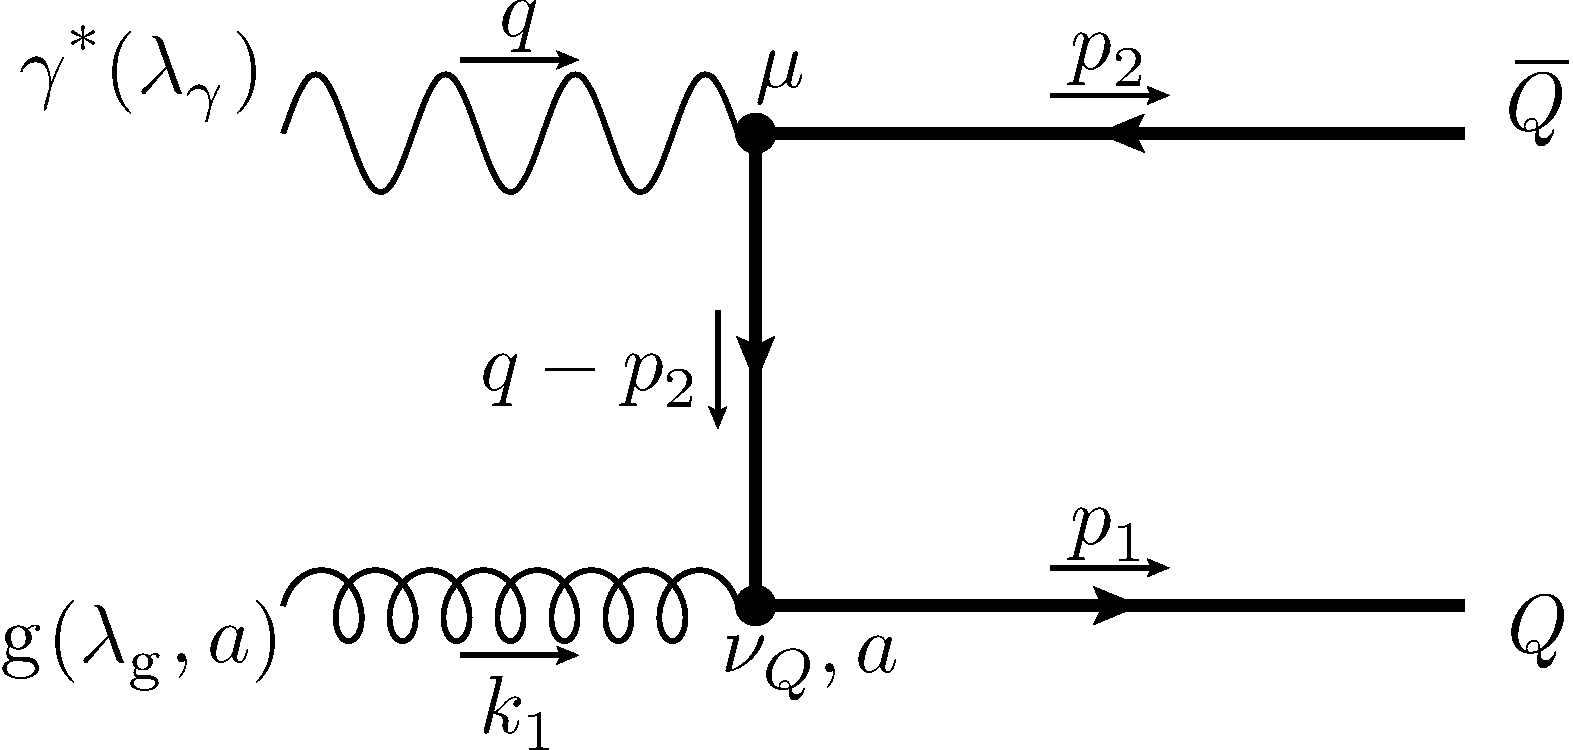
\includegraphics[width=\textwidth]{pyfeyn/lo-a}
		\caption{$i\Md^{(LO)}_{1,\mu}$}
	\end{subfigure}\hspace{.15\textwidth}%
	\begin{subfigure}[t]{.4\textwidth}
		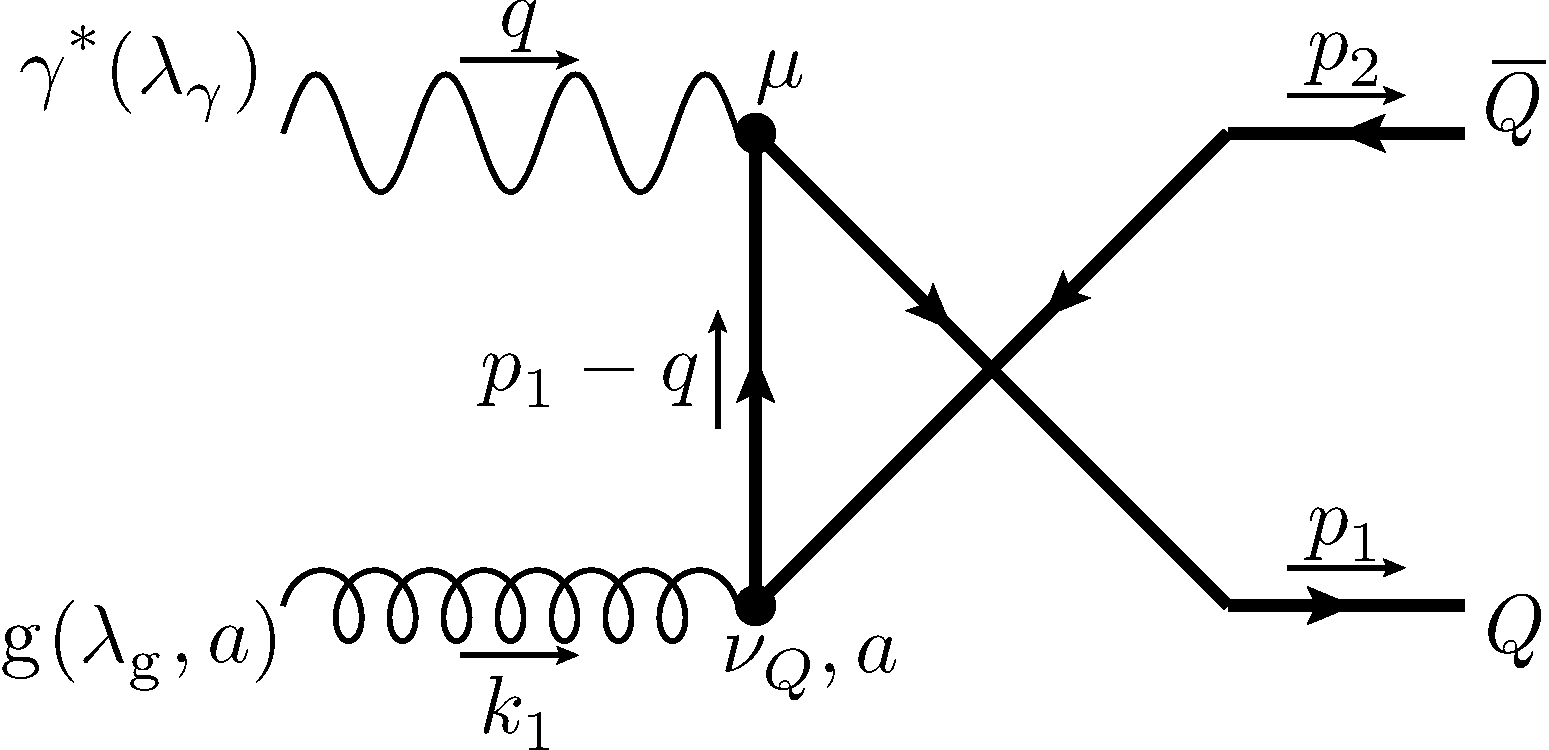
\includegraphics[width=\textwidth]{pyfeyn/lo-b}
		\caption{$i\Md^{(LO)}_{2,\mu}$}
	\end{subfigure}
	\caption{LO contributions}\label{fig:FeynLO}
\end{figure}

formula:
\begin{align}
i\Md^{(LO)}_{1,\mu} &= \bar u(p_1)(igT_a\gamma^{\nu_Q})\frac{i(\slashed{q}-\slashed{p}_2+m)}{u_1}(-i e e_H \gamma_\mu)v(p_2)\varepsilon^{(\lambda_{\Pg})}_{\nu_Q}(k_1)\\
i\Md^{(LO)}_{2,\mu} &= \bar u(p_1)(-i e e_H \gamma_\mu)\frac{i(\slashed{p}_1-\slashed{q}+m)}{t_1}(igT_a\gamma^{\nu_Q})v(p_2)\varepsilon^{(\lambda_{\Pg})}_{\nu_Q}(k_1)
\end{align}

color space:
\begin{equation}
\abs{\Md^{(LO)}_{1,\mu}+\Md^{(LO)}_{2,\mu}}^2 \sim \tr(T_a T_a) = N_c C_F
\end{equation}

%resulting in:
%\begin{align}
%B_{G,QED} &=\\
%B_{L,QED} &=  -\frac{4q^2(st_1u_1-m^2(t_1+u_1)^2)}{{s'}^2t_1u_1}\\
%\Delta B_{QED} &= \frac 1 {s' t_1^2u_1^2}\left(-2 {m^2} {s'} ({t_1}^3 + {t_1}^2 {u_1} + {t_1} {u_1}^2 + {u_1}^3)+\right.\nonumber\\
% &\left. {t_1} {u_1} ({s'}^2 ({t_1} + {u_1}) + ({t_1} - {u_1})^2 ({t_1} + {u_1}) + {s'} ({t_1}^2 + {u_1}^2) + 
%    {q^2} (-({t_1} - {u_1})^2 + {s'} ({t_1} + {u_1})))\right)
%\end{align}
%in accordance with \cite{Laenen1993162} and \cite{Marco}\fxerror{insert}


\section[Next-to-leading Order: O(a aS2)]{Next-to-leading Order: $O(\alpha \alpha_S^2)$}
\subsection{Light Quark Contributions}
\begin{equation}
\Pggx(q) + \Pq(k_1) \rightarrow \PaQ(p_2) + \PQ(p_1) + \Pq(k_2)
\end{equation}

diagramatic:
\begin{figure}[ht!]
	\centering
	\begin{subfigure}[t]{.4\textwidth}
		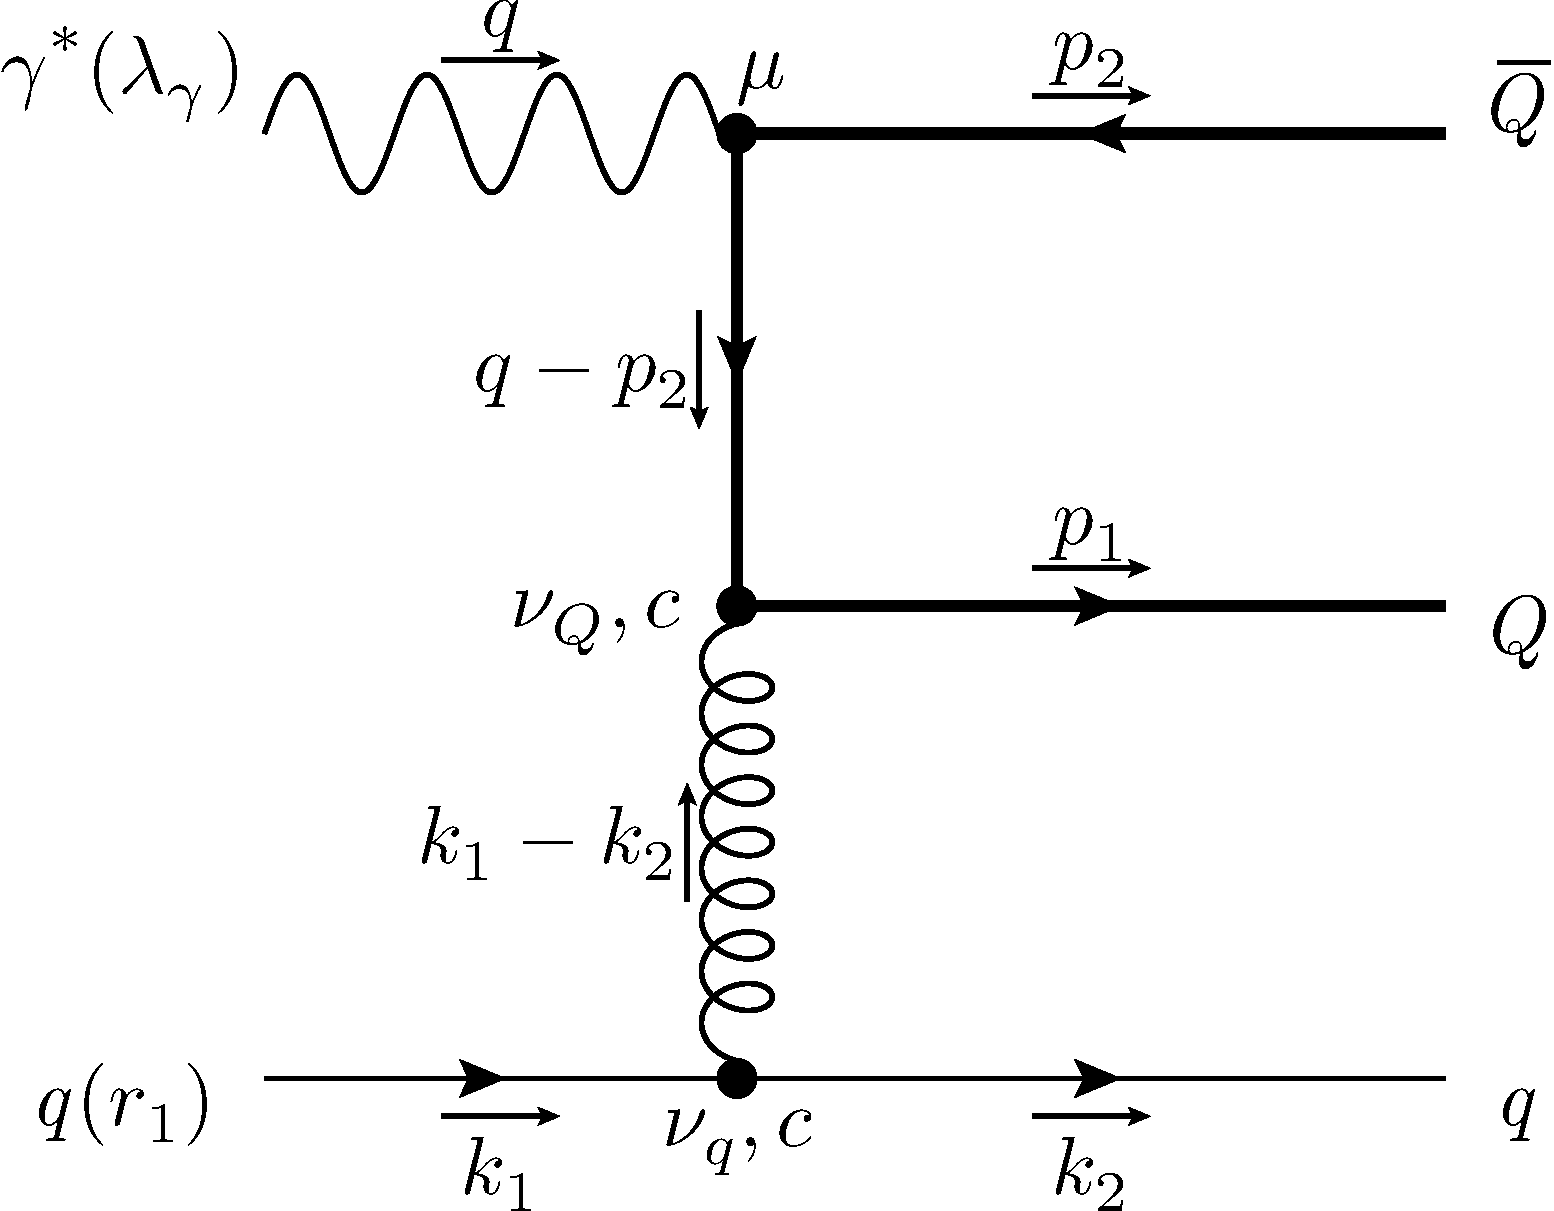
\includegraphics[width=\textwidth]{pyfeyn/nlo-q-a}
		\caption{$i\Md^{(NLO,q)}_{1,\mu}$}
	\end{subfigure}\hspace{.15\textwidth}%
	\begin{subfigure}[t]{.4\textwidth}
		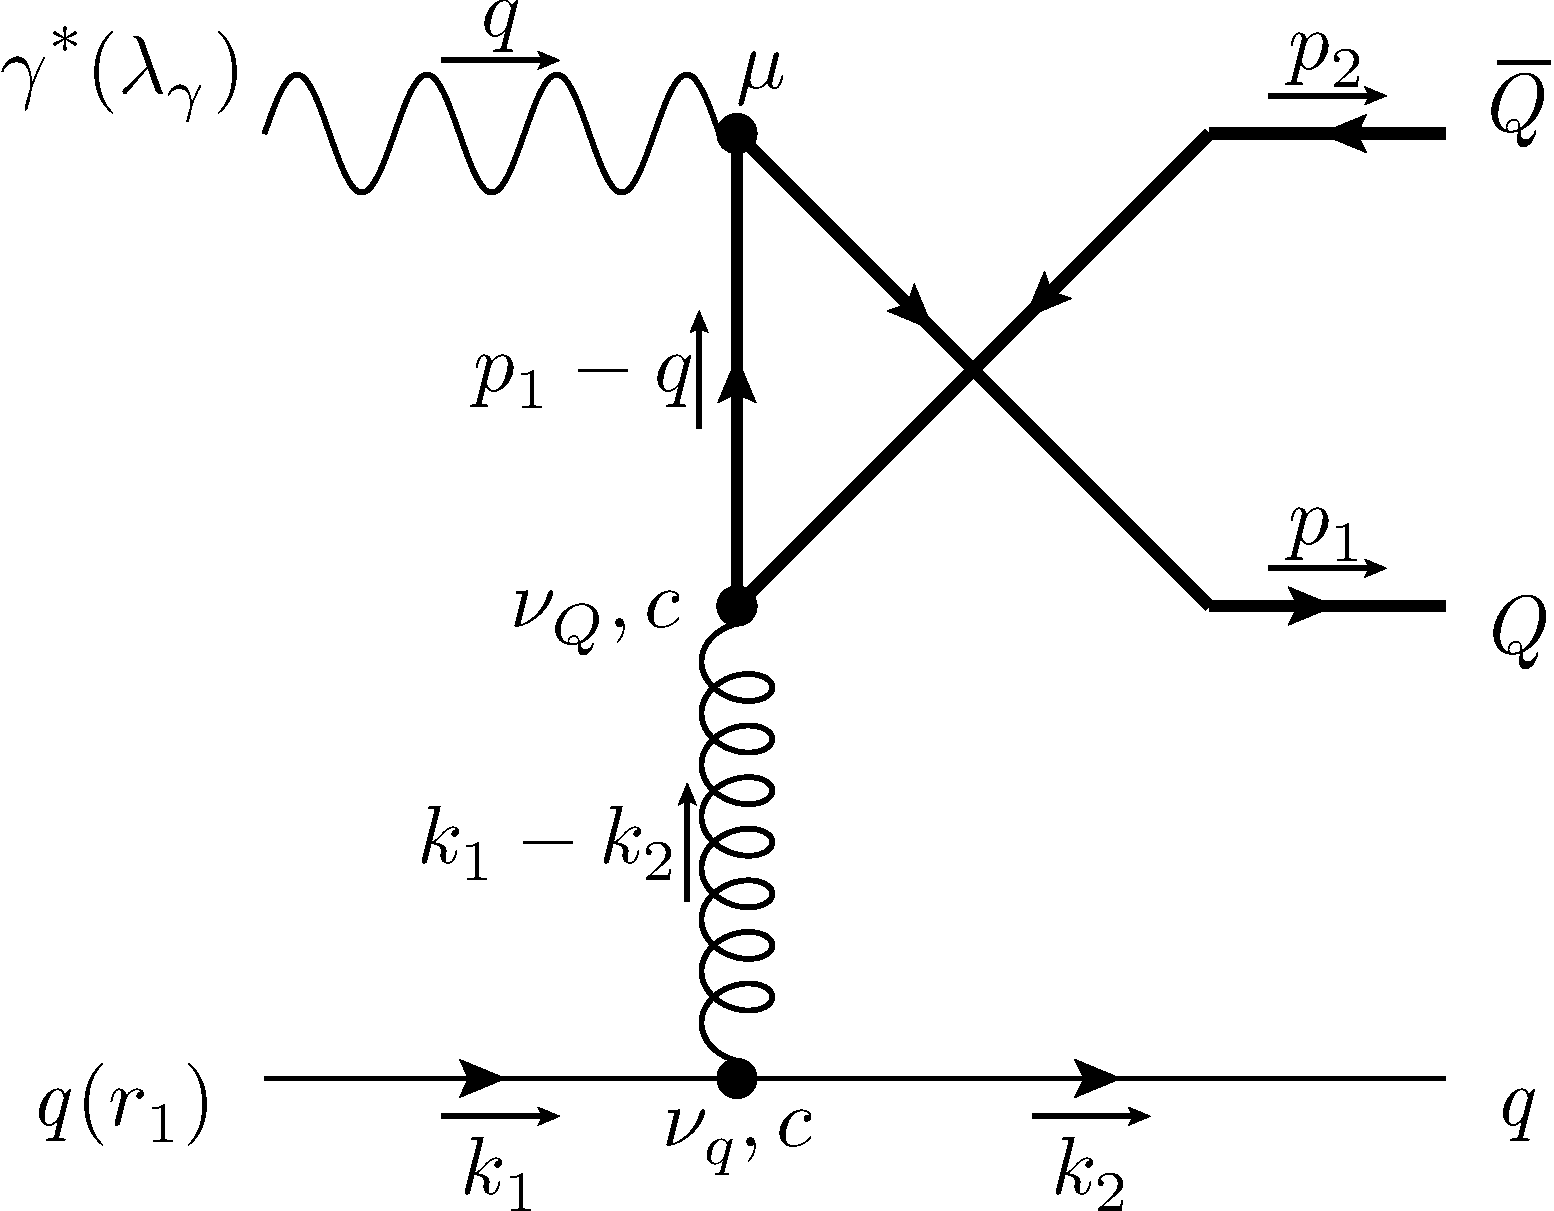
\includegraphics[width=\textwidth]{pyfeyn/nlo-q-b}
		\caption{$i\Md^{(NLO,q)}_{2,\mu}$}
	\end{subfigure}\\
	\begin{subfigure}[t]{.42\textwidth}
		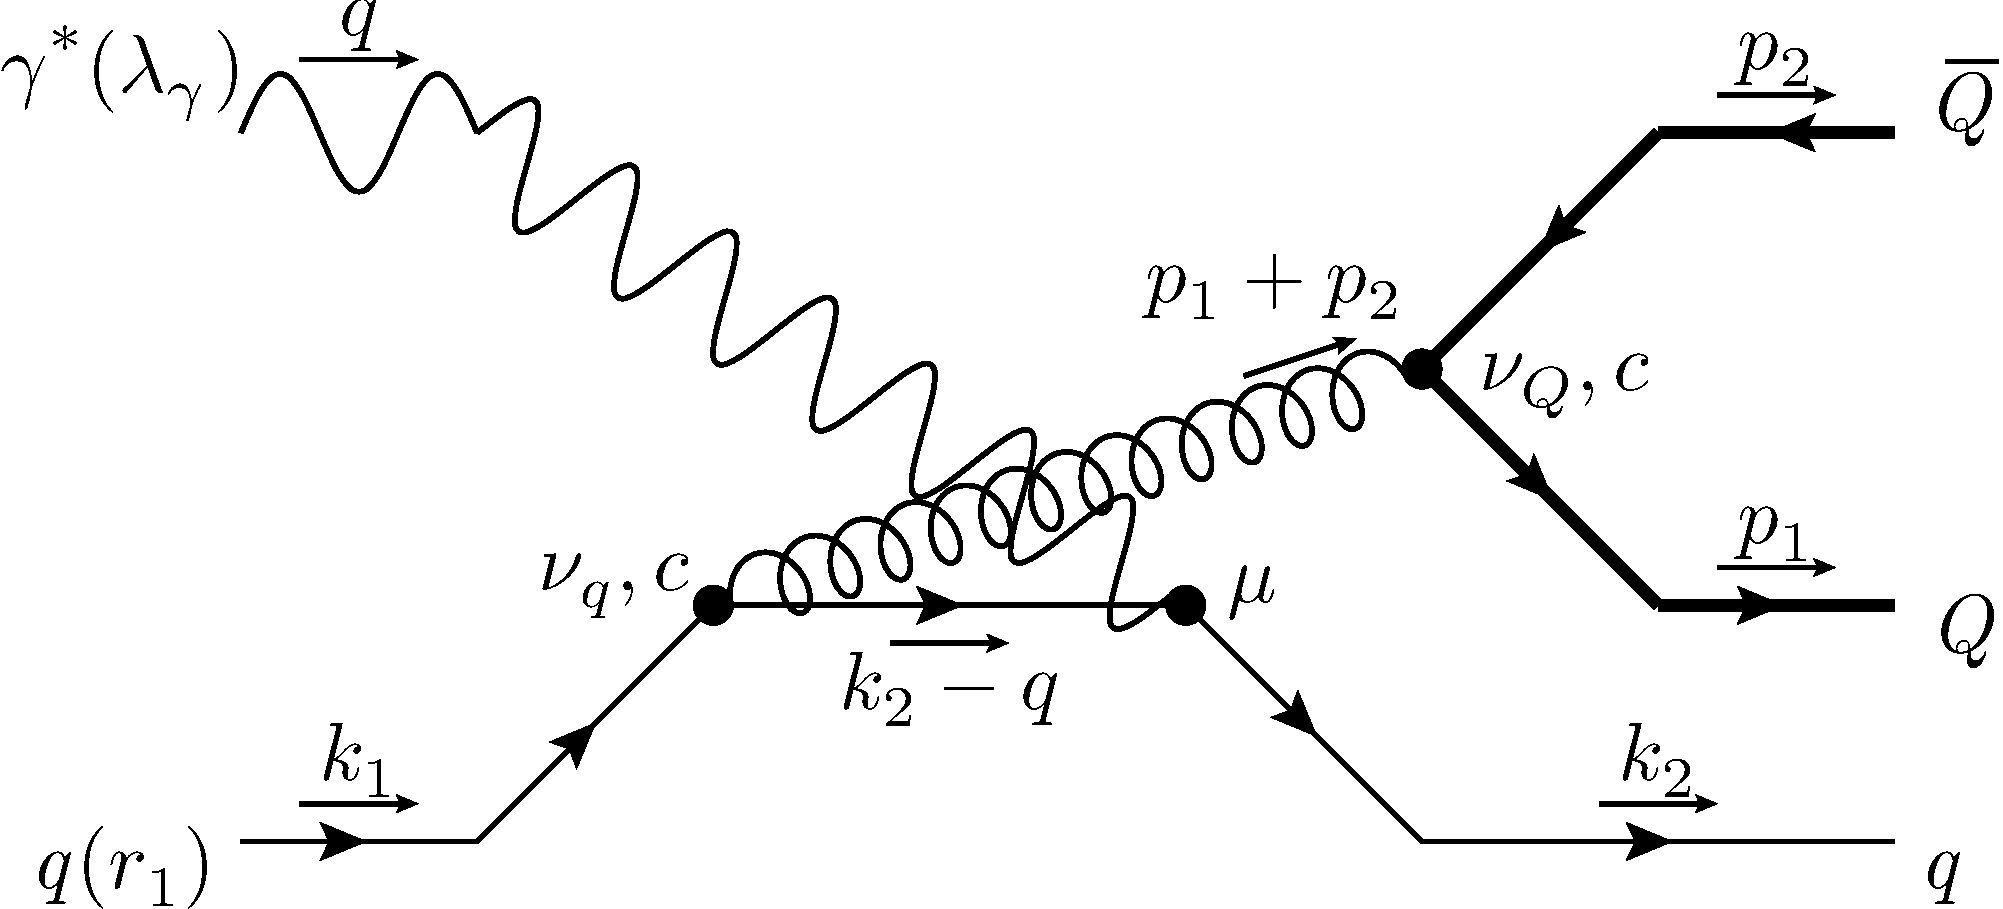
\includegraphics[width=\textwidth]{pyfeyn/nlo-q-c}
		\caption{$i\Md^{(NLO,q)}_{3,\mu}$}
	\end{subfigure}\hspace{.1\textwidth}%
	\begin{subfigure}[t]{.42\textwidth}
		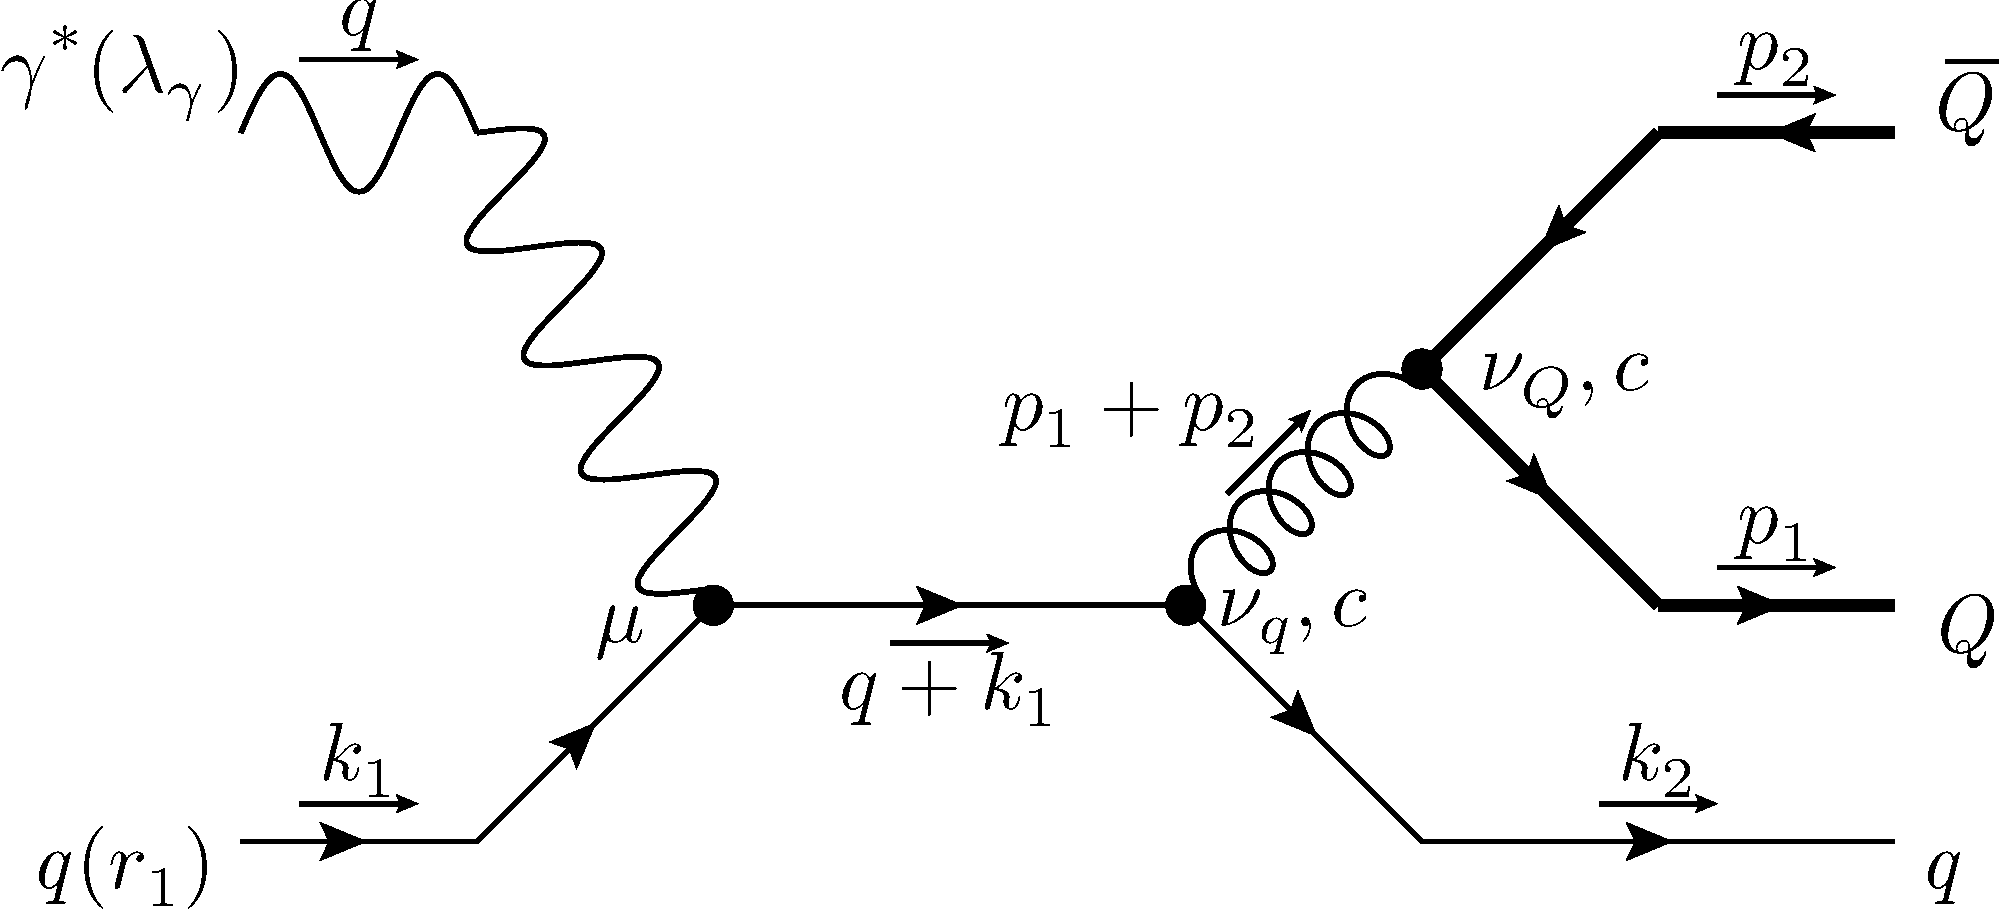
\includegraphics[width=\textwidth]{pyfeyn/nlo-q-d}
		\caption{$i\Md^{(NLO,q)}_{4,\mu}$}
	\end{subfigure}
	\caption{NLO contributions by light quarks}\label{fig:FeynNLOq}
\end{figure}

formula:
\begin{align}
i\Md^{(NLO,q)}_{1,\mu} &= \bar u_Q(p_1)(igT_c\gamma^{\nu_Q})\frac{i(\slashed{q}-\slashed{p}_2+m)}{u_1}(-i e e_H \gamma_\mu)v_Q(p_2)\cdot \nonumber\\
 &\hspace{20pt}\frac{-ig_{\nu_Q,\nu_q}}{t'} \cdot \bar u_q(k_2)(igT_c\gamma^{\nu_q})u^{(r_1)}_q(k_1)\\
i\Md^{(NLO,q)}_{2,\mu} &= \bar u_Q(p_1)(-i e e_H \gamma_\mu)\frac{i(\slashed{p}_1-\slashed{q}+m)}{u_7}(igT_c\gamma^{\nu_Q})v_Q(p_2) \cdot \nonumber\\
&\hspace{20pt} \frac{-ig_{\nu_Q,\nu_q}}{t'} \cdot \bar u_q(k_2)(igT_c\gamma^{\nu_q})u^{(r_1)}_q(k_1)\\
i\Md^{(NLO,q)}_{3,\mu} &= \bar u_Q(p_1)(igT_c\gamma^{\nu_Q})v_Q(p_2) \cdot \frac{-ig_{\nu_Q,\nu_q}}{s_5} \cdot \nonumber\\
 &\hspace{20pt}\bar u_q(k_2)(-i e e_L \gamma_\mu)\frac{i(\slashed{k}_2-\slashed{q})}{u'}(igT_c\gamma^{\nu_q})u^{(r_1)}_q(k_1)\\
i\Md^{(NLO,q)}_{4,\mu} &= \bar u_Q(p_1)(igT_c\gamma^{\nu_Q})v_Q(p_2) \cdot \frac{-ig_{\nu_Q,\nu_q}}{s_5} \cdot \nonumber\\
 &\hspace{20pt}\bar u_q(k_2)(igT_c\gamma^{\nu_q})\frac{i(\slashed{k}_1+\slashed{q})}{s}(-i e e_L \gamma_\mu)u^{(r_1)}_q(k_1)
\end{align}

color space:
\begin{equation}
\abs{\Md^{(NLO,q)}_{1,\mu}+\Md^{(NLO,q)}_{2,\mu}+\Md^{(NLO,q)}_{3,\mu}+\Md^{(NLO,q)}_{4,\mu}}^2 \sim \tr(T_c T_d)\tr(T_c T_d) = \frac 1 2 N_c C_F
\end{equation}


\subsection{Gluon Bremsstrahlung}
\begin{equation}
\Pggx(q) + \Pg(k_1) \rightarrow \PaQ(p_2) + \PQ(p_1) + \Pg(k_2)
\end{equation}

diagramatic:
\begin{figure}[ht!]
	\centering
	\begin{subfigure}[t]{.4\textwidth}
		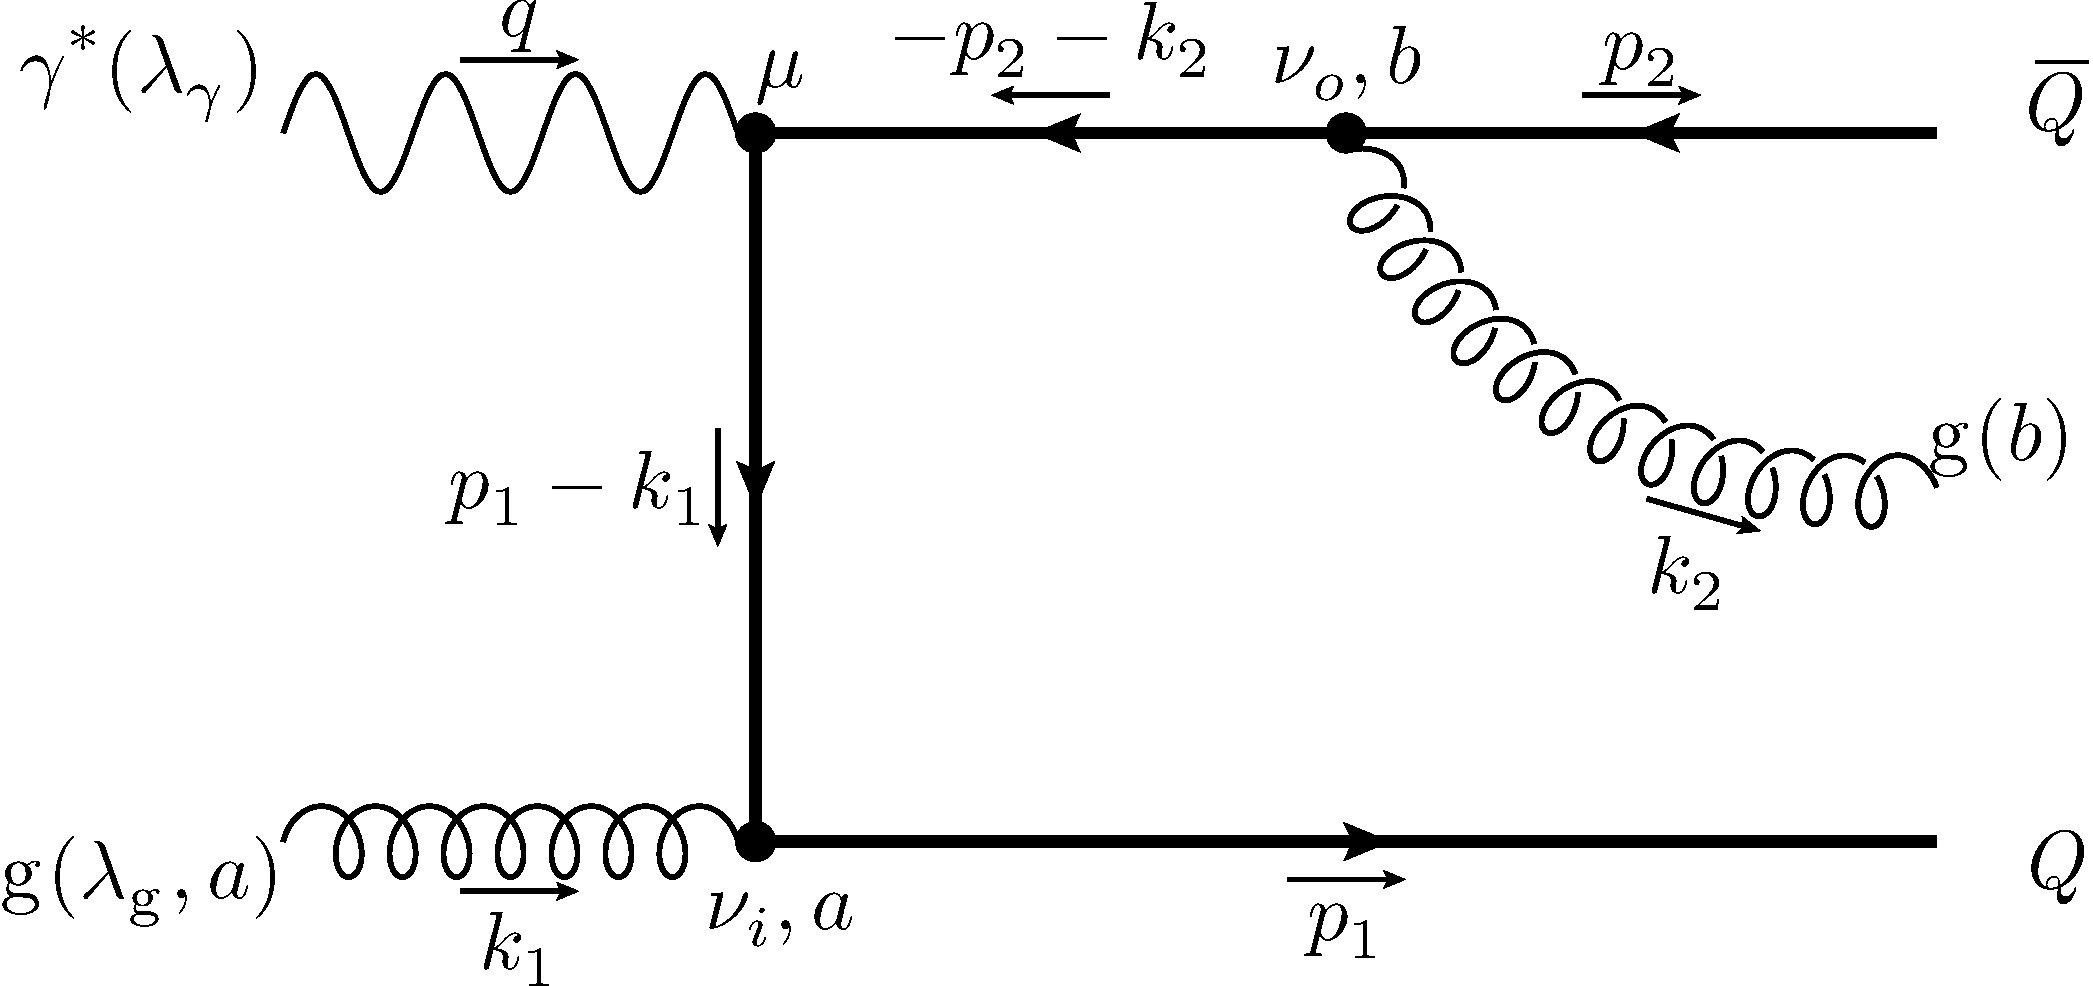
\includegraphics[width=\textwidth]{pyfeyn/nlo-g-1}
		\caption{$i\Md^{(NLO,g)}_{1,\mu}$}
	\end{subfigure}\hspace{.15\textwidth}%
	\begin{subfigure}[t]{.4\textwidth}
		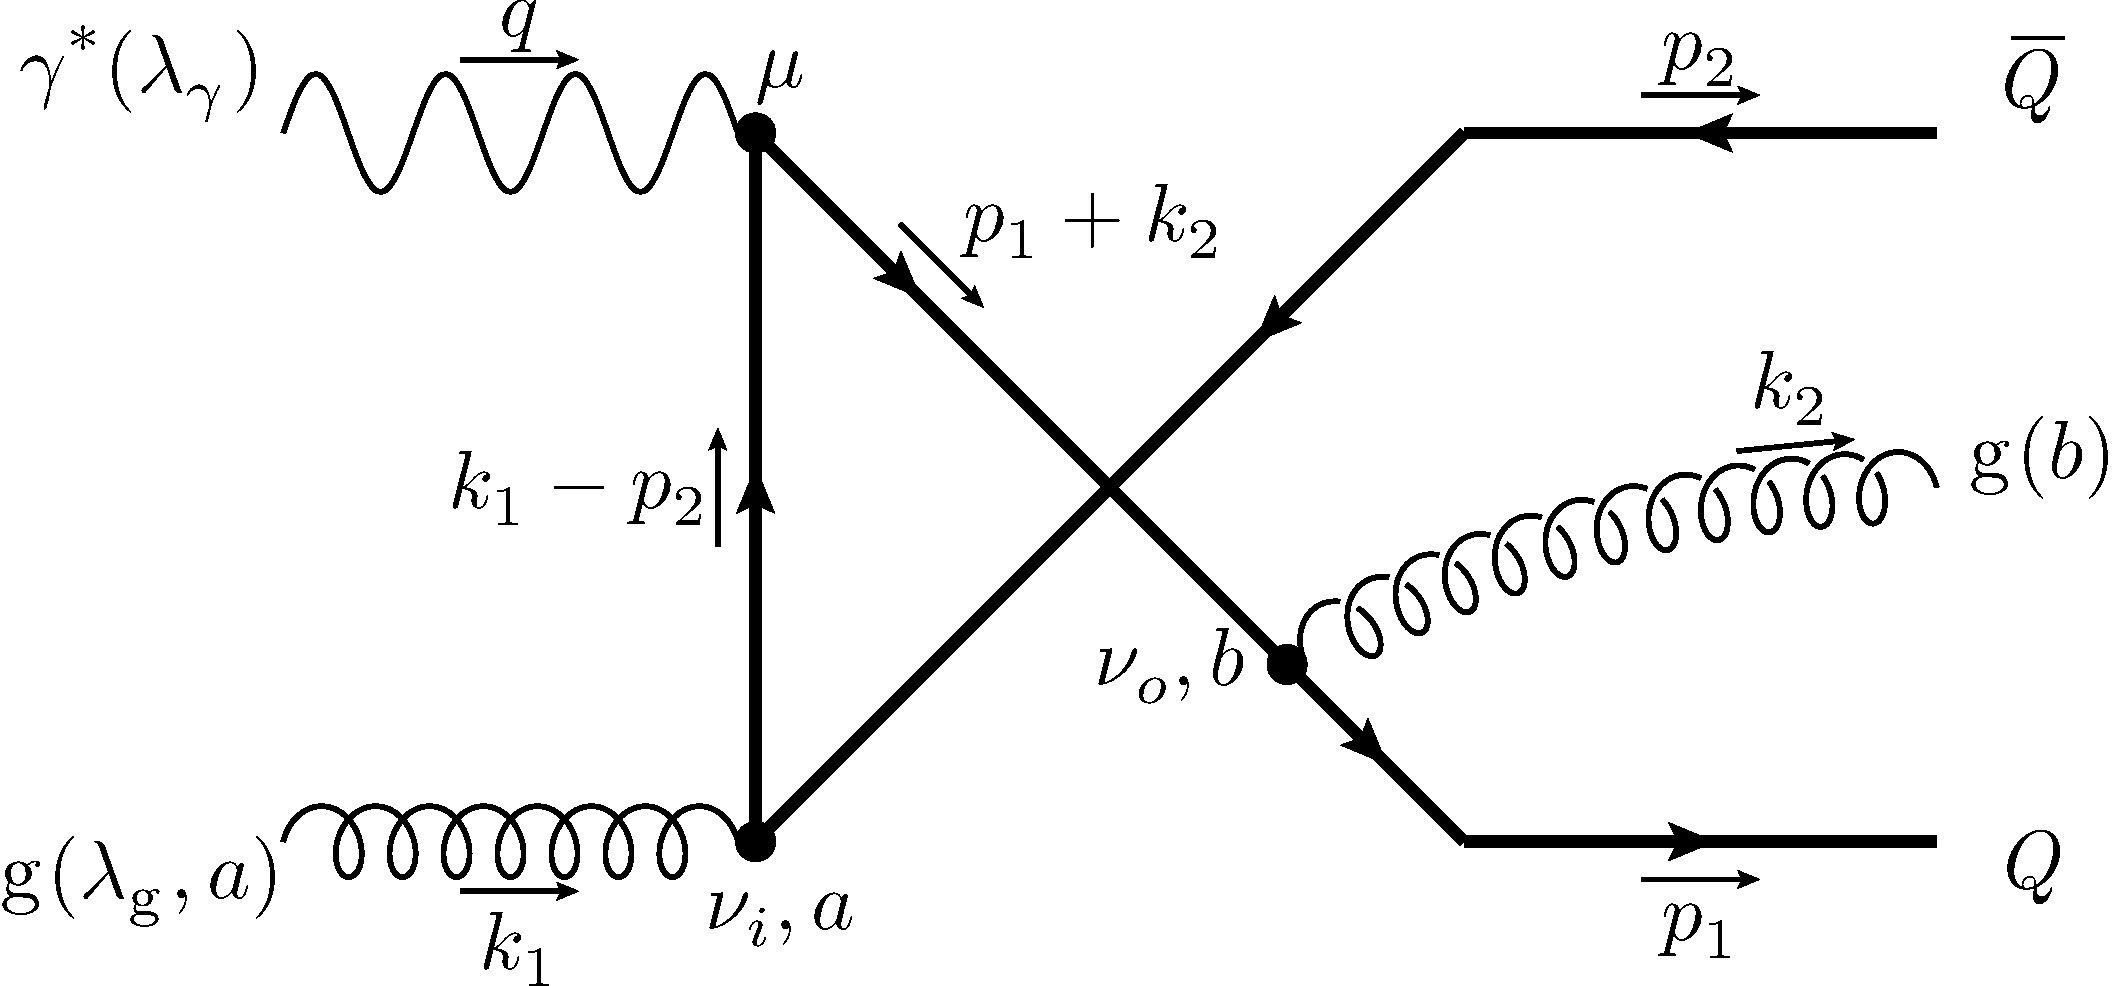
\includegraphics[width=\textwidth]{pyfeyn/nlo-g-2}
		\caption{$i\Md^{(NLO,g)}_{2,\mu}$}
	\end{subfigure}\\
	\begin{subfigure}[t]{.42\textwidth}
		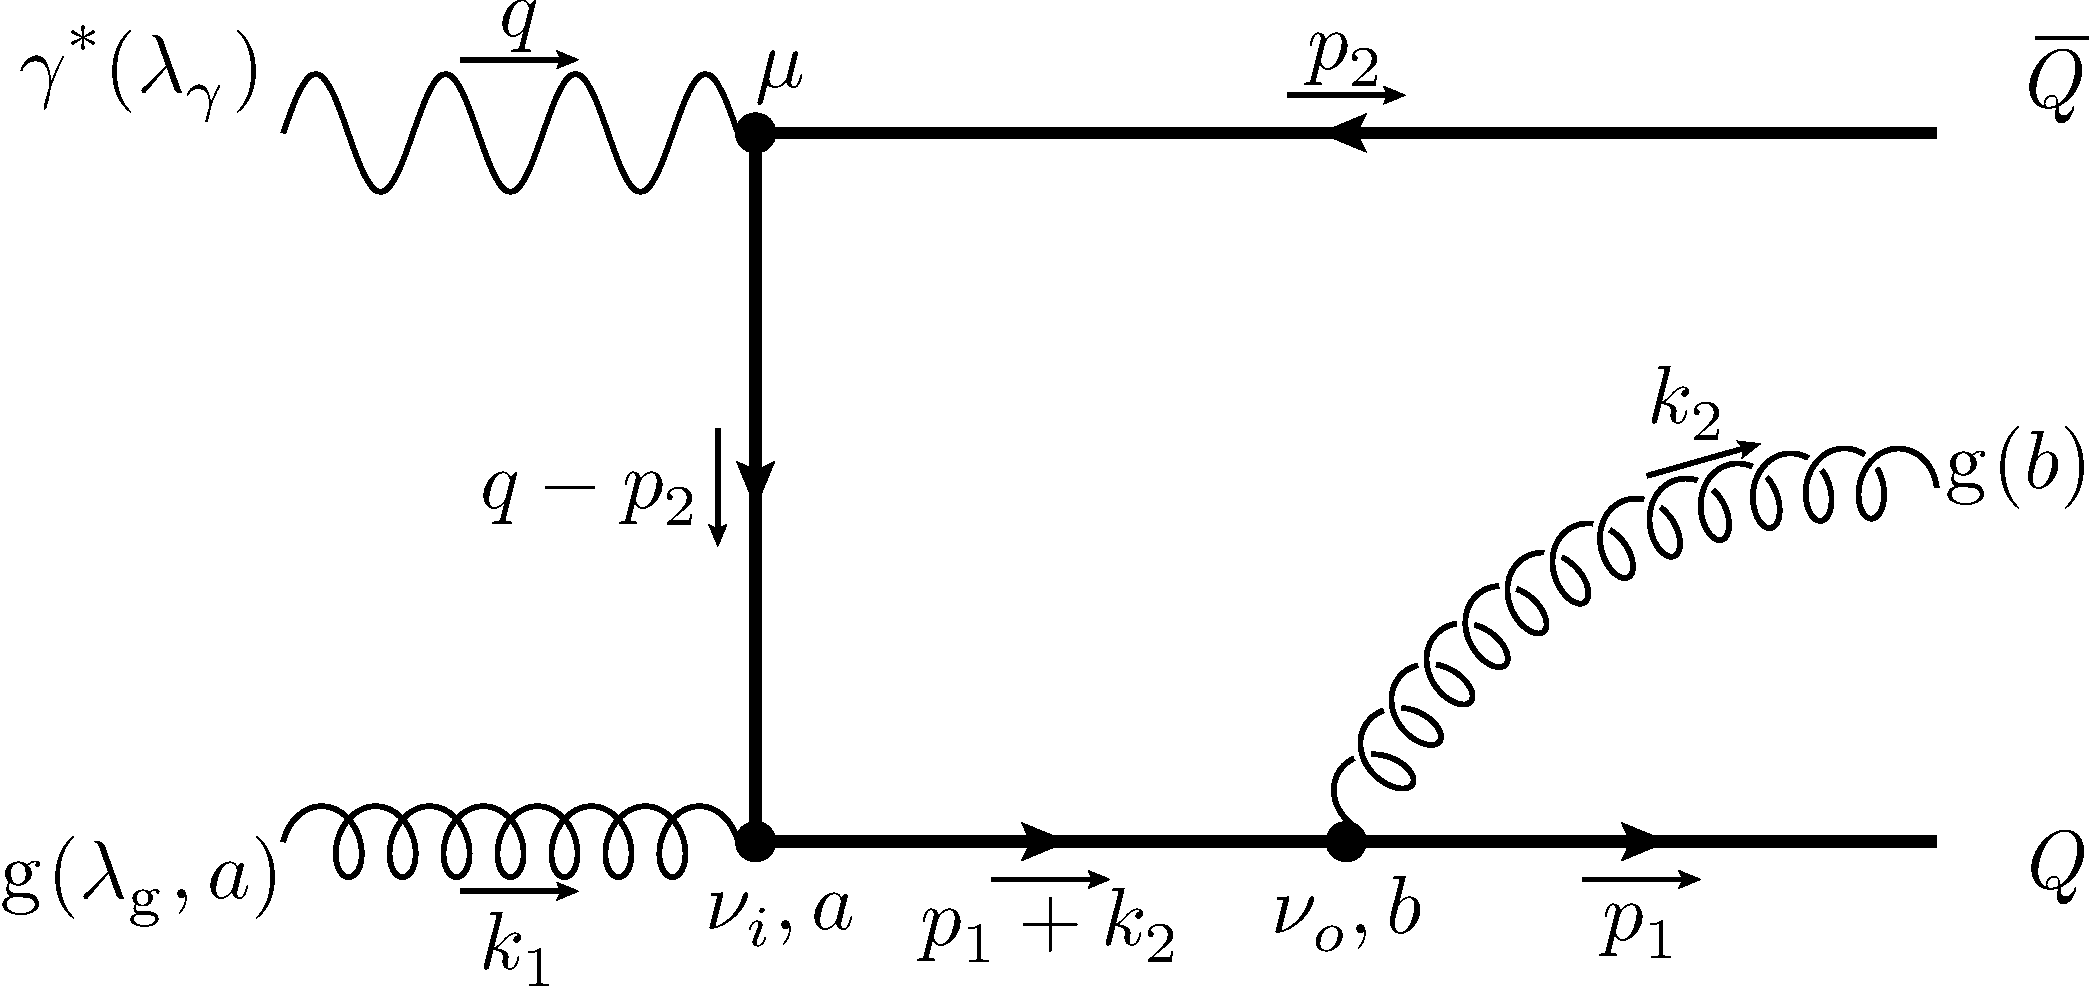
\includegraphics[width=\textwidth]{pyfeyn/nlo-g-3}
		\caption{$i\Md^{(NLO,g)}_{3,\mu}$}
	\end{subfigure}\hspace{.1\textwidth}%
	\begin{subfigure}[t]{.42\textwidth}
		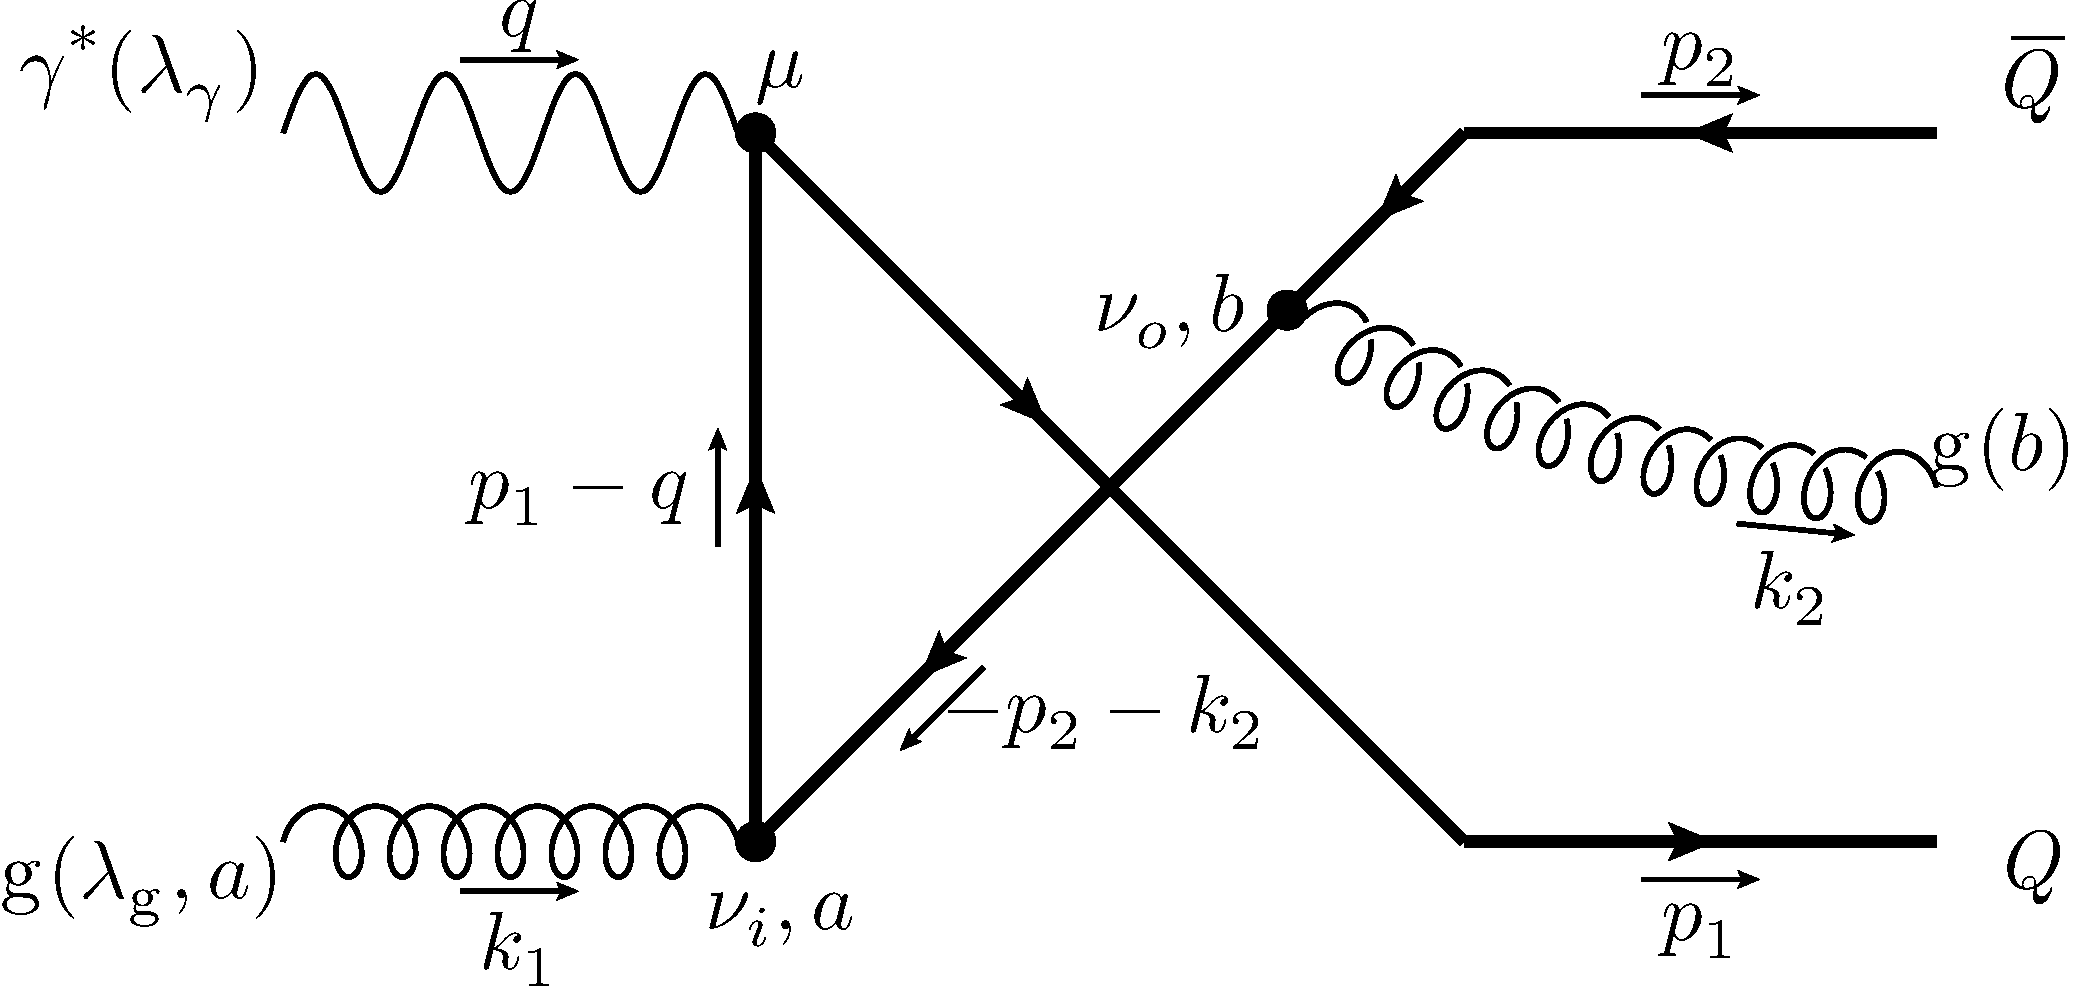
\includegraphics[width=\textwidth]{pyfeyn/nlo-g-4}
		\caption{$i\Md^{(NLO,g)}_{4,\mu}$}
	\end{subfigure}\\
	\begin{subfigure}[t]{.4\textwidth}
		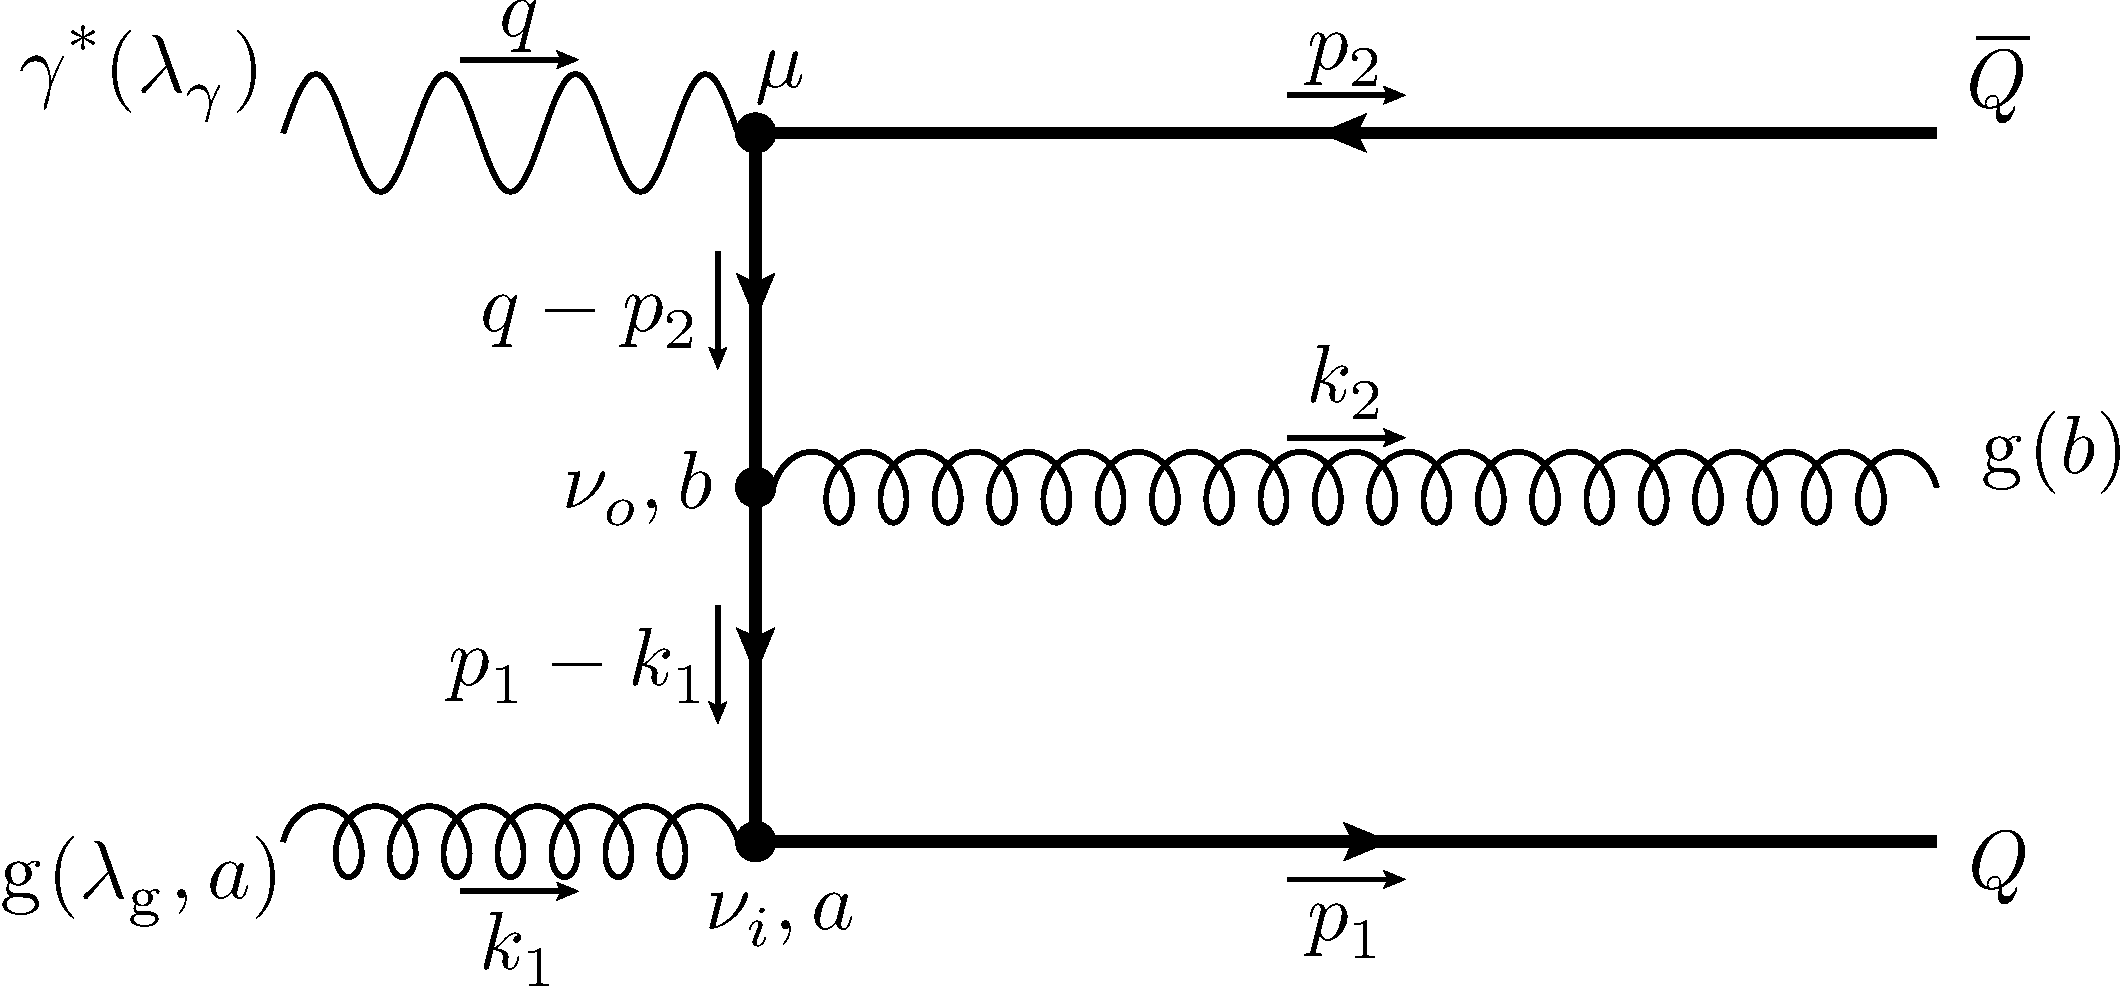
\includegraphics[width=\textwidth]{pyfeyn/nlo-g-5}
		\caption{$i\Md^{(NLO,g)}_{5,\mu}$}
	\end{subfigure}\hspace{.15\textwidth}%
	\begin{subfigure}[t]{.4\textwidth}
		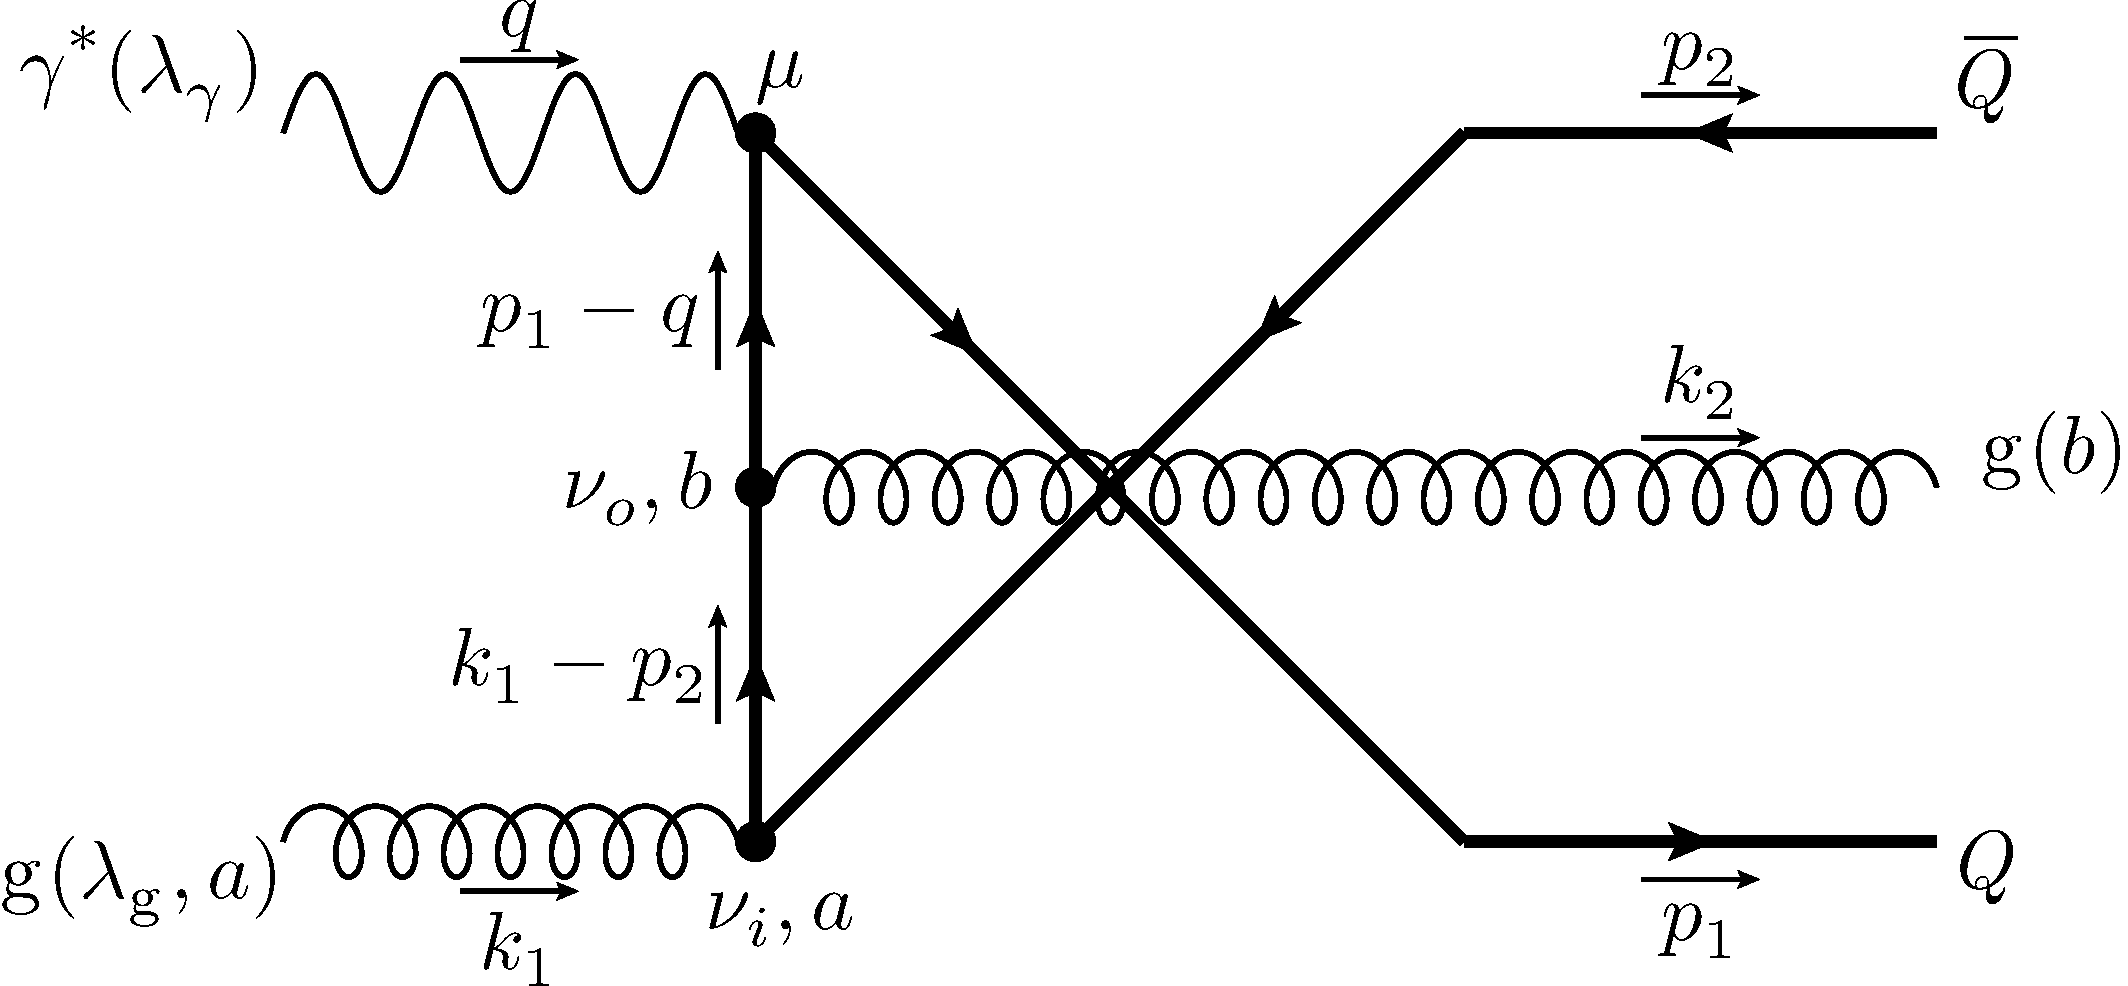
\includegraphics[width=\textwidth]{pyfeyn/nlo-g-6}
		\caption{$i\Md^{(NLO,g)}_{6,\mu}$}
	\end{subfigure}\\
	\begin{subfigure}[t]{.42\textwidth}
		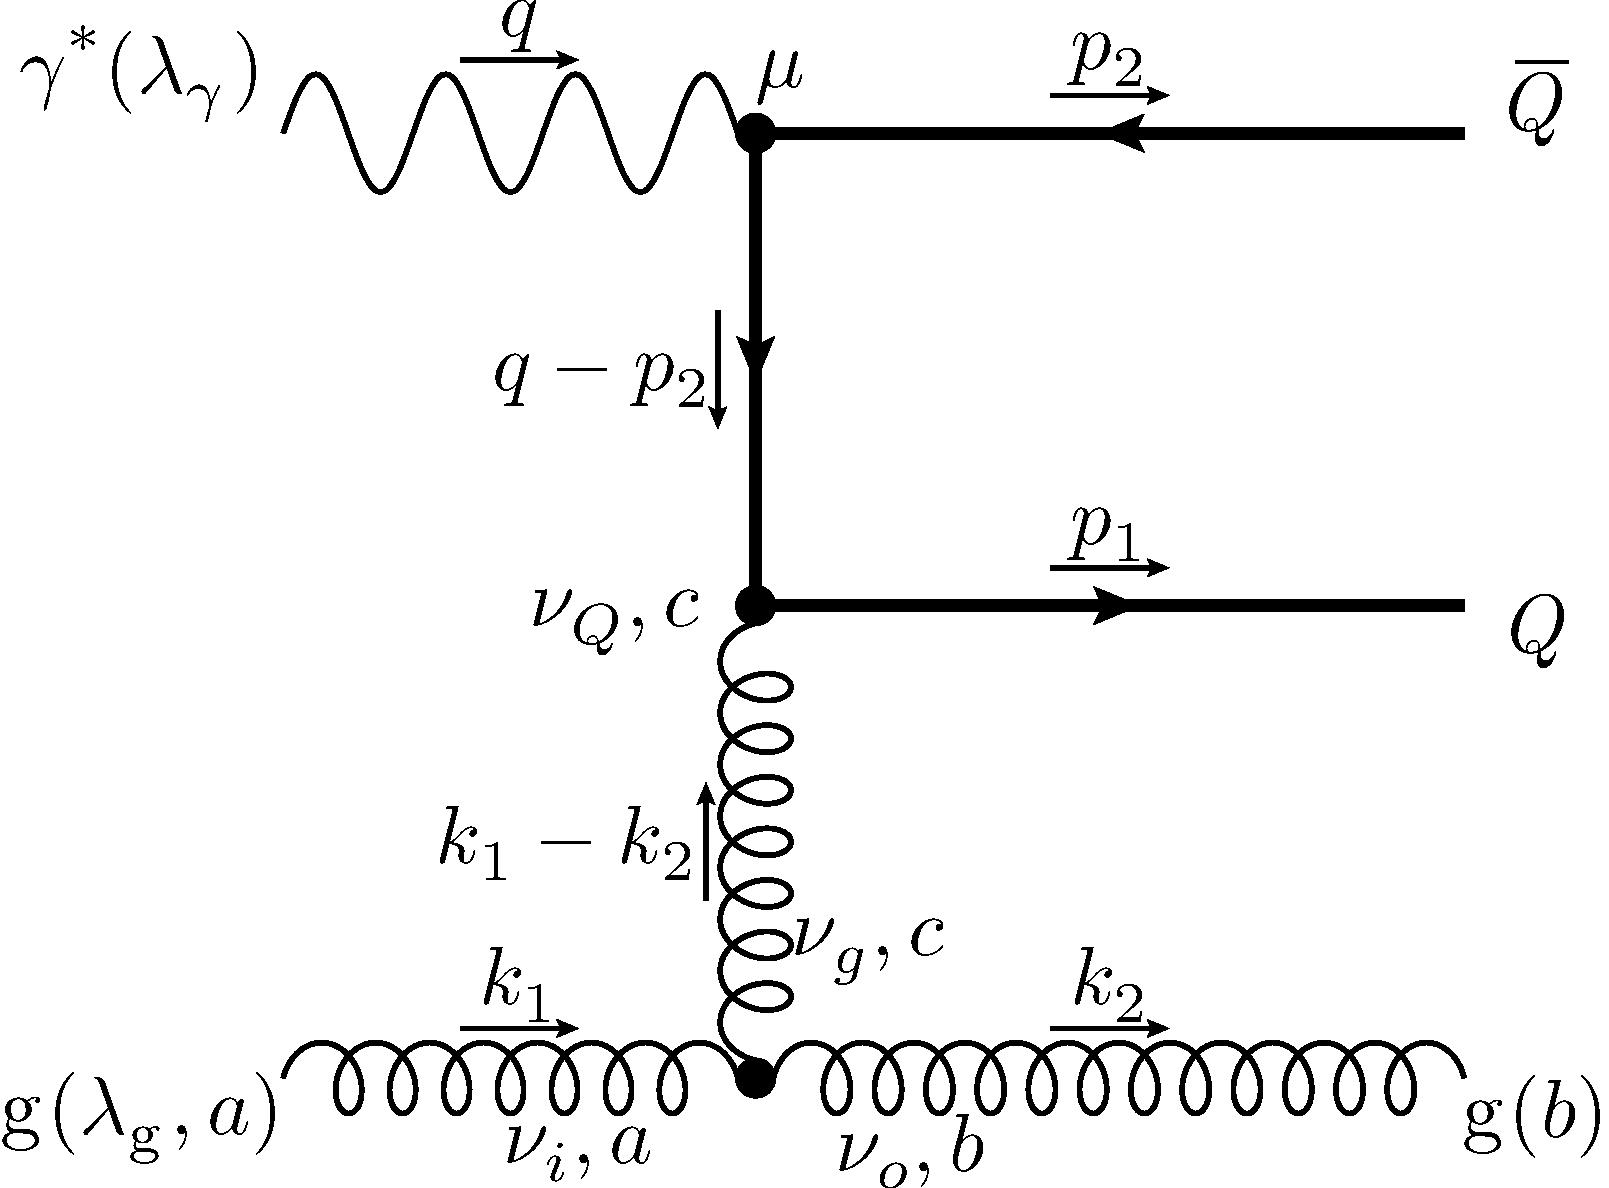
\includegraphics[width=\textwidth]{pyfeyn/nlo-g-7}
		\caption{$i\Md^{(NLO,g)}_{7,\mu}$}
	\end{subfigure}\hspace{.1\textwidth}%
	\begin{subfigure}[t]{.42\textwidth}
		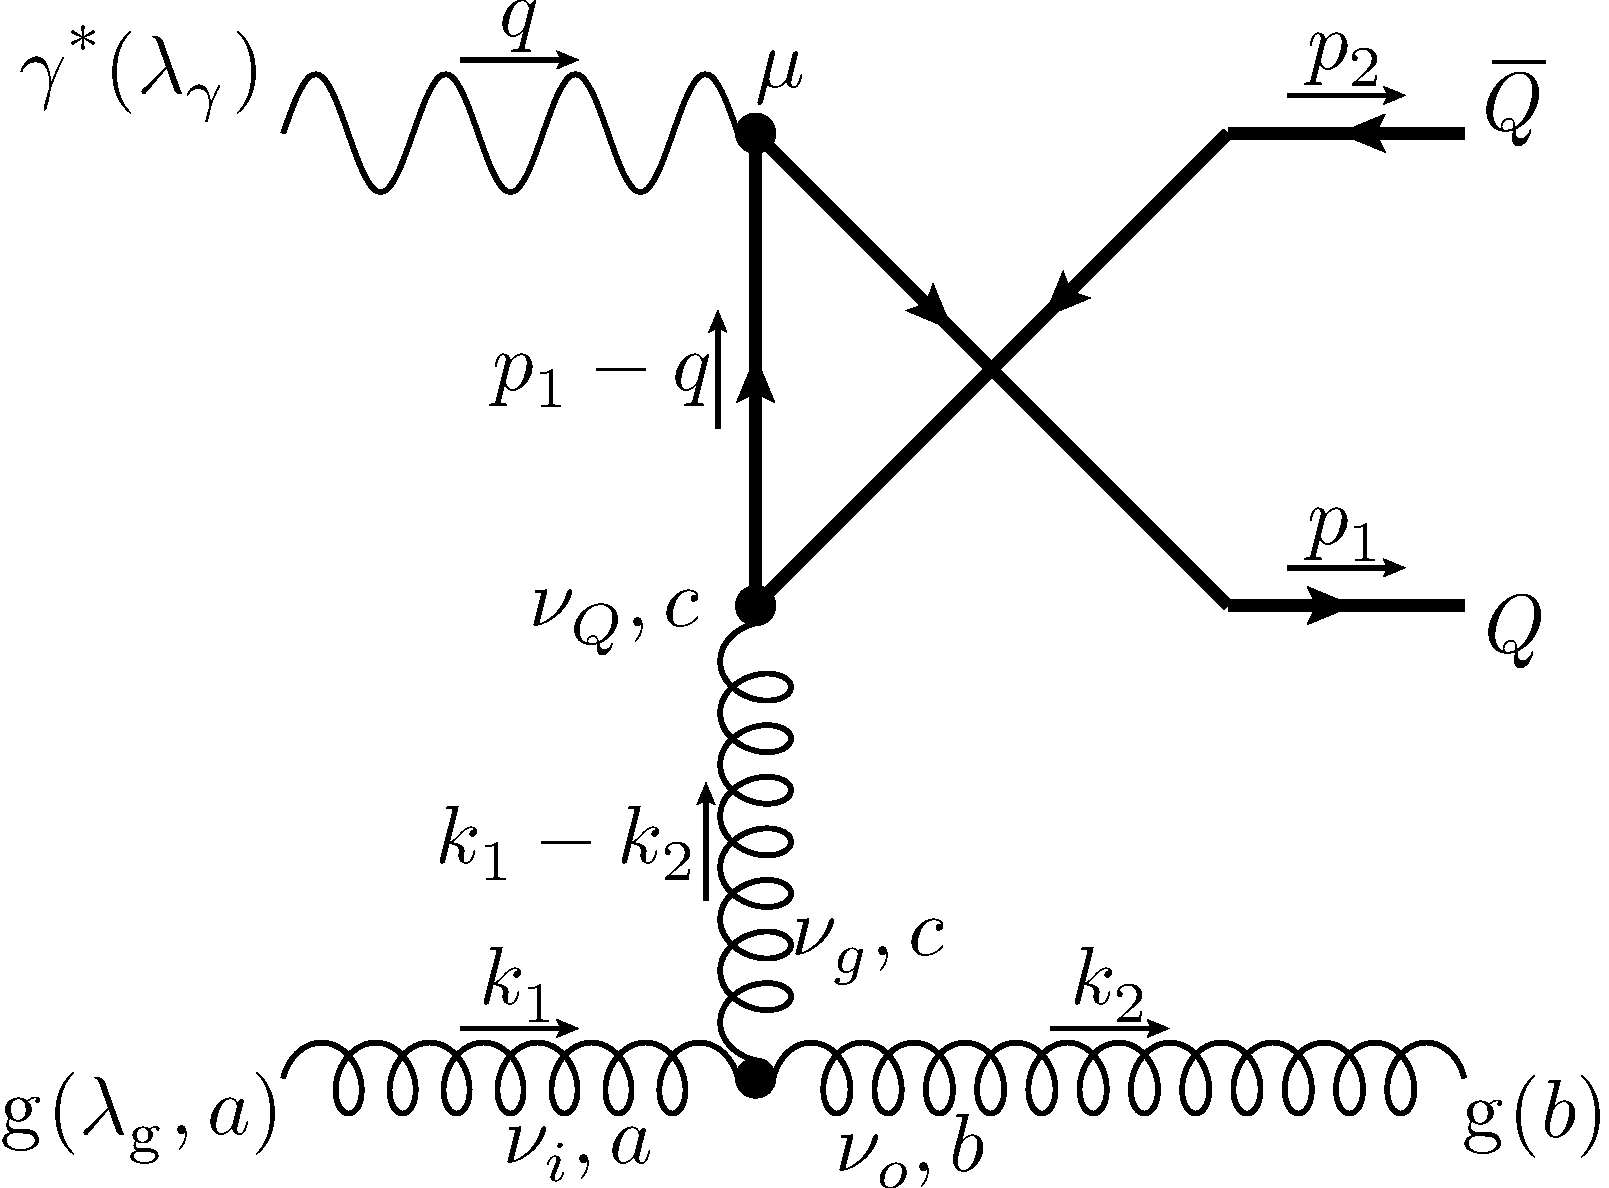
\includegraphics[width=\textwidth]{pyfeyn/nlo-g-8}
		\caption{$i\Md^{(NLO,g)}_{8,\mu}$}
	\end{subfigure}
	\caption{NLO contributions by gluon bremsstrahlung}\label{fig:FeynNLOg}
\end{figure}

formula:
\begin{align}
i\Md^{(NLO,g)}_{1,\mu} &= \bar u(p_1)(igT_a\gamma^{\nu_i})\frac{i(\slashed{p}_1-\slashed{k}_1+m)}{u_6}(-i e e_H \gamma_\mu)\cdot\nonumber\\
 &\hspace{40pt}\frac{i(-\slashed{p}_2-\slashed{k}_2+m)}{s_3}(igT_b\gamma^{\nu_o})v(p_2)\varepsilon^{(\lambda_{\Pg})}_{\nu_i}(k_1)\varepsilon_{\nu_o}(k_2)\\
i\Md^{(NLO,g)}_{2,\mu} &= \bar u(p_1)(igT_b\gamma^{\nu_o})\frac{i(\slashed{p}_1+\slashed{k}_2+m)}{s_4}(-i e e_H \gamma_\mu)\cdot\nonumber\\
 &\hspace{40pt}\frac{i(\slashed{k}_1-\slashed{p}_2+m)}{t_1}(igT_a\gamma^{\nu_i})v(p_2)\varepsilon^{(\lambda_{\Pg})}_{\nu_i}(k_1)\varepsilon_{\nu_o}(k_2)\\
i\Md^{(NLO,g)}_{3,\mu} &= \bar u(p_1)(igT_b\gamma^{\nu_o})\frac{i(\slashed{p}_1+\slashed{k}_2+m)}{s_4}(igT_a\gamma^{\nu_i})\cdot\nonumber\\
 &\hspace{40pt}\frac{i(\slashed{q}-\slashed{p}_2+m)}{u_1}(-i e e_H \gamma_\mu)v(p_2)\varepsilon^{(\lambda_{\Pg})}_{\nu_i}(k_1)\varepsilon_{\nu_o}(k_2)\\
i\Md^{(NLO,g)}_{4,\mu} &= \bar u(p_1)(-i e e_H \gamma_\mu)\frac{i(\slashed{p}_1-\slashed{q}+m)}{u_7}(igT_a\gamma^{\nu_i})\cdot\nonumber\\
 &\hspace{40pt}\frac{i(-\slashed{p}_2-\slashed{k}_2+m)}{s_3}(igT_b\gamma^{\nu_o})v(p_2)\varepsilon^{(\lambda_{\Pg})}_{\nu_i}(k_1)\varepsilon_{\nu_o}(k_2)\\
i\Md^{(NLO,g)}_{5,\mu} &= \bar u(p_1)(igT_a\gamma^{\nu_i})\frac{i(\slashed{p}_1-\slashed{k}_1+m)}{u_6}(igT_b\gamma^{\nu_o})\cdot\nonumber\\
 &\hspace{40pt}\frac{i(\slashed{q}-\slashed{p}_2+m)}{u_1}(-i e e_H \gamma_\mu)v(p_2)\varepsilon^{(\lambda_{\Pg})}_{\nu_i}(k_1)\varepsilon_{\nu_o}(k_2)\\
i\Md^{(NLO,g)}_{6,\mu} &= \bar u(p_1)(-i e e_H \gamma_\mu)\frac{i(\slashed{p}_1-\slashed{q}+m)}{u_7}(igT_b\gamma^{\nu_o})\cdot\nonumber\\
 &\hspace{40pt}\frac{i(\slashed{k}_1-\slashed{p}_2+m)}{t_1}(igT_a\gamma^{\nu_i})v(p_2)\varepsilon^{(\lambda_{\Pg})}_{\nu_i}(k_1)\varepsilon_{\nu_o}(k_2)\\
i\Md^{(NLO,g)}_{7,\mu} &= \bar u(p_1)(igT_c\gamma^{\nu_Q})\frac{i(\slashed{q}-\slashed{p}_2+m)}{u_1}(-i e e_H \gamma_\mu)v(p_2)\cdot\frac{-g_{\nu_Q,\nu_g}}{t'}\cdot\varepsilon^{(\lambda_{\Pg})}_{\nu_i}(k_1)\varepsilon_{\nu_o}(k_2)\cdot\nonumber\\
 &\hspace{30pt}\left(gf^{acb}\left(g^{\nu_o,\nu_i}(k_1+k_2)^{\nu_g}+g^{\nu_i,\nu_g}(k_2-2k_1)^{\nu_o}+g^{\nu_g,\nu_o}(k_1-2k_2)^{\nu_i}\right)\right)\\
i\Md^{(NLO,g)}_{8,\mu} &= \bar u(p_1)(-i e e_H \gamma_\mu)\frac{i(\slashed{p}_1-\slashed{q}+m)}{u_7}(igT_c\gamma^{\nu_Q})v(p_2)\cdot\frac{-g_{\nu_Q,\nu_g}}{t'}\cdot\varepsilon^{(\lambda_{\Pg})}_{\nu_i}(k_1)\varepsilon_{\nu_o}(k_2)\cdot\nonumber\\
 &\hspace{30pt}\left(gf^{acb}\left(g^{\nu_o,\nu_i}(k_1+k_2)^{\nu_g}+g^{\nu_i,\nu_g}(k_2-2k_1)^{\nu_o}+g^{\nu_g,\nu_o}(k_1-2k_2)^{\nu_i}\right)\right)
\end{align}

color space:
\begin{align}
&\sum\limits_{j=1}^6\abs{\Md^{(NLO,g)}_{j,\mu}}^2 + \Md^{(NLO,g)}_{1,\mu}\left(\Md^{(NLO,g)}_{4,\mu'}+\Md^{(NLO,g)}_{5,\mu'}\right)^*+\Md^{(NLO,g)}_{3,\mu}\left(\Md^{(NLO,g)}_{6,\mu'}\right)^*+\nonumber\\
&\Md^{(NLO,g)}_{2,\mu}\left(\Md^{(NLO,g)}_{3,\mu'}+\Md^{(NLO,g)}_{6,\mu'}\right)^*+\Md^{(NLO,g)}_{4,\mu}\left(\Md^{(NLO,g)}_{5,\mu'}\right)^*\nonumber\\
&\sim\tr(T_aT_aT_bT_b) = N_C C_F^2\\
&\Md^{(NLO,g)}_{1,\mu}\left(\Md^{(NLO,g)}_{2,\mu'}+\Md^{(NLO,g)}_{3,\mu'}+\Md^{(NLO,g)}_{6,\mu'}\right)^*+\nonumber\\
&\left(\Md^{(NLO,g)}_{2,\mu}+\Md^{(NLO,g)}_{3,\mu}\right)\left(\Md^{(NLO,g)}_{4,\mu'}+\Md^{(NLO,g)}_{5,\mu'}\right)^*+\nonumber\\
&\left(\Md^{(NLO,g)}_{4,\mu}+\Md^{(NLO,g)}_{5,\mu}\right)\left(\Md^{(NLO,g)}_{6,\mu'}\right)^*\nonumber\\
&\sim\tr(T_aT_bT_aT_b) = N_C C_F \left(C_F - \frac{C_A}{2}\right)\\
&\left(\Md^{(NLO,g)}_{2,\mu}+\Md^{(NLO,g)}_{3,\mu}+\Md^{(NLO,g)}_{6,\mu}\right)\left(\Md^{(NLO,g)}_{7,\mu'}+\Md^{(NLO,g)}_{8,\mu'}\right)^*\nonumber\\
&\sim-if_{bda}\tr(T_aT_bT_d) = \frac 1 2 N_C C_F C_A\\
&\left(\Md^{(NLO,g)}_{1,\mu}+\Md^{(NLO,g)}_{4,\mu}+\Md^{(NLO,g)}_{5,\mu}\right)\left(\Md^{(NLO,g)}_{7,\mu'}+\Md^{(NLO,g)}_{8,\mu'}\right)^*\nonumber\\
&\sim-if_{bda}\tr(T_bT_aT_d) = if_{bda}\tr(T_aT_bT_d)=-\frac 1 2 N_C C_F C_A\\
&\abs{\Md^{(NLO,g)}_{7,\mu}+\Md^{(NLO,g)}_{8,\mu}}^2 \nonumber\\
&\sim f_{acb}f_{adb}\tr(T_cT_d) = N_C C_F C_A
\end{align}

\pagebreak
To get the polarisation sums right, one has to subtract the contributions of the Faddeev-Popov ghosts\cite{FADDEEV196729,QFT}:

diagramatic:
\begin{figure}[ht!]
	\centering
	\begin{subfigure}[t]{.4\textwidth}
		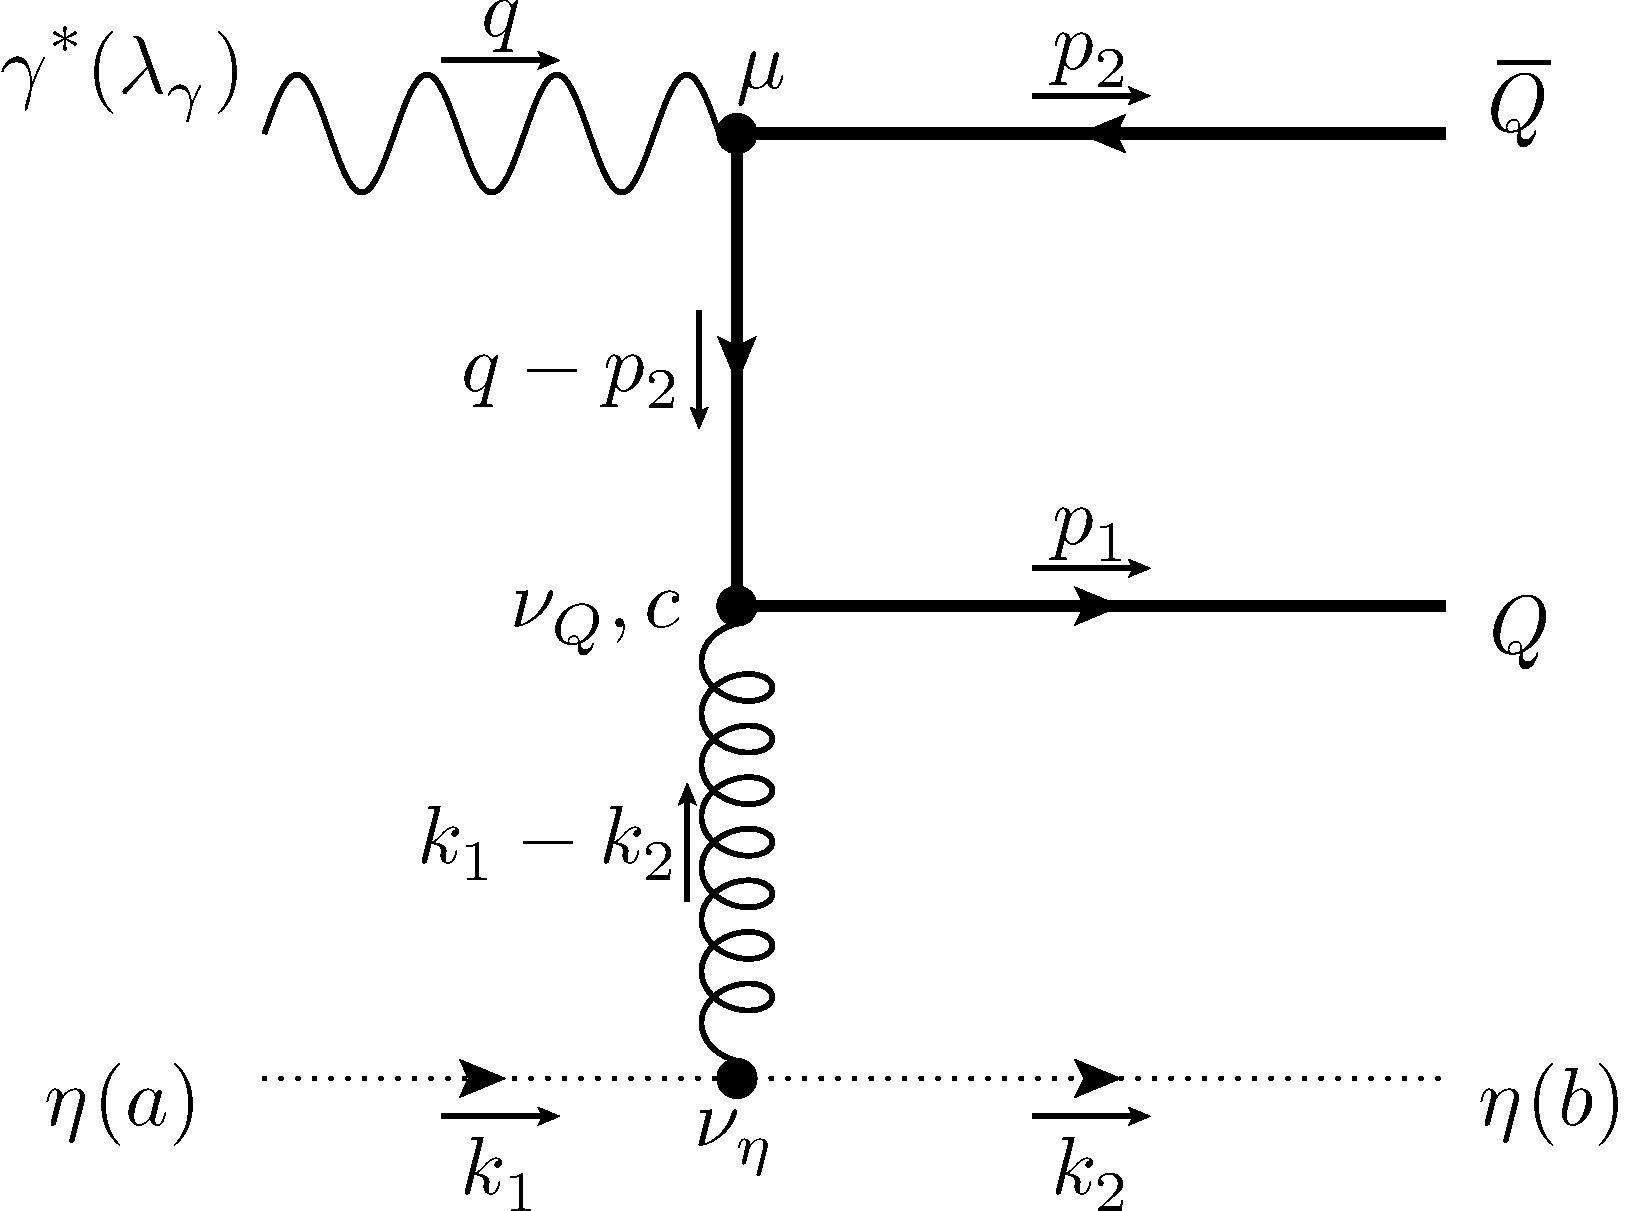
\includegraphics[width=\textwidth]{pyfeyn/nlo-gh-1}
		\caption{$i\Md^{(NLO,\Pgh)}_{1,\mu}$}
	\end{subfigure}\hspace{.15\textwidth}%
	\begin{subfigure}[t]{.4\textwidth}
		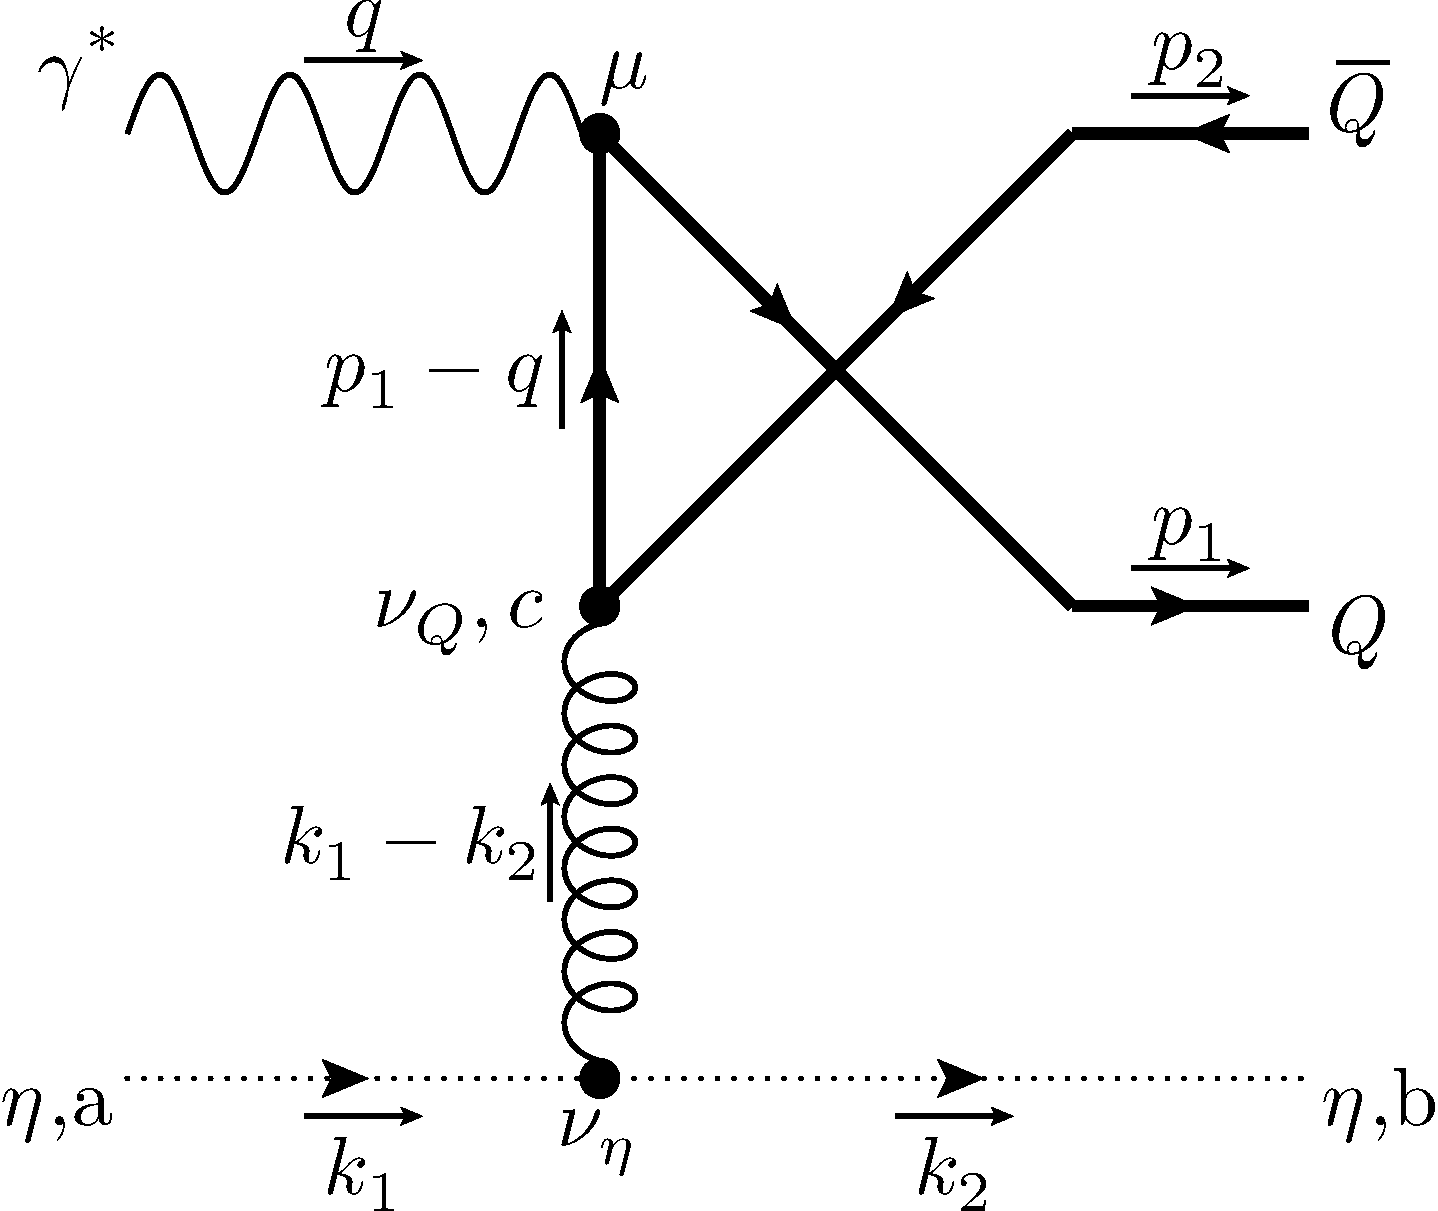
\includegraphics[width=\textwidth]{pyfeyn/nlo-gh-2}
		\caption{$i\Md^{(NLO,\Pgh)}_{2,\mu}$}
	\end{subfigure}\\
	\begin{subfigure}[t]{.42\textwidth}
		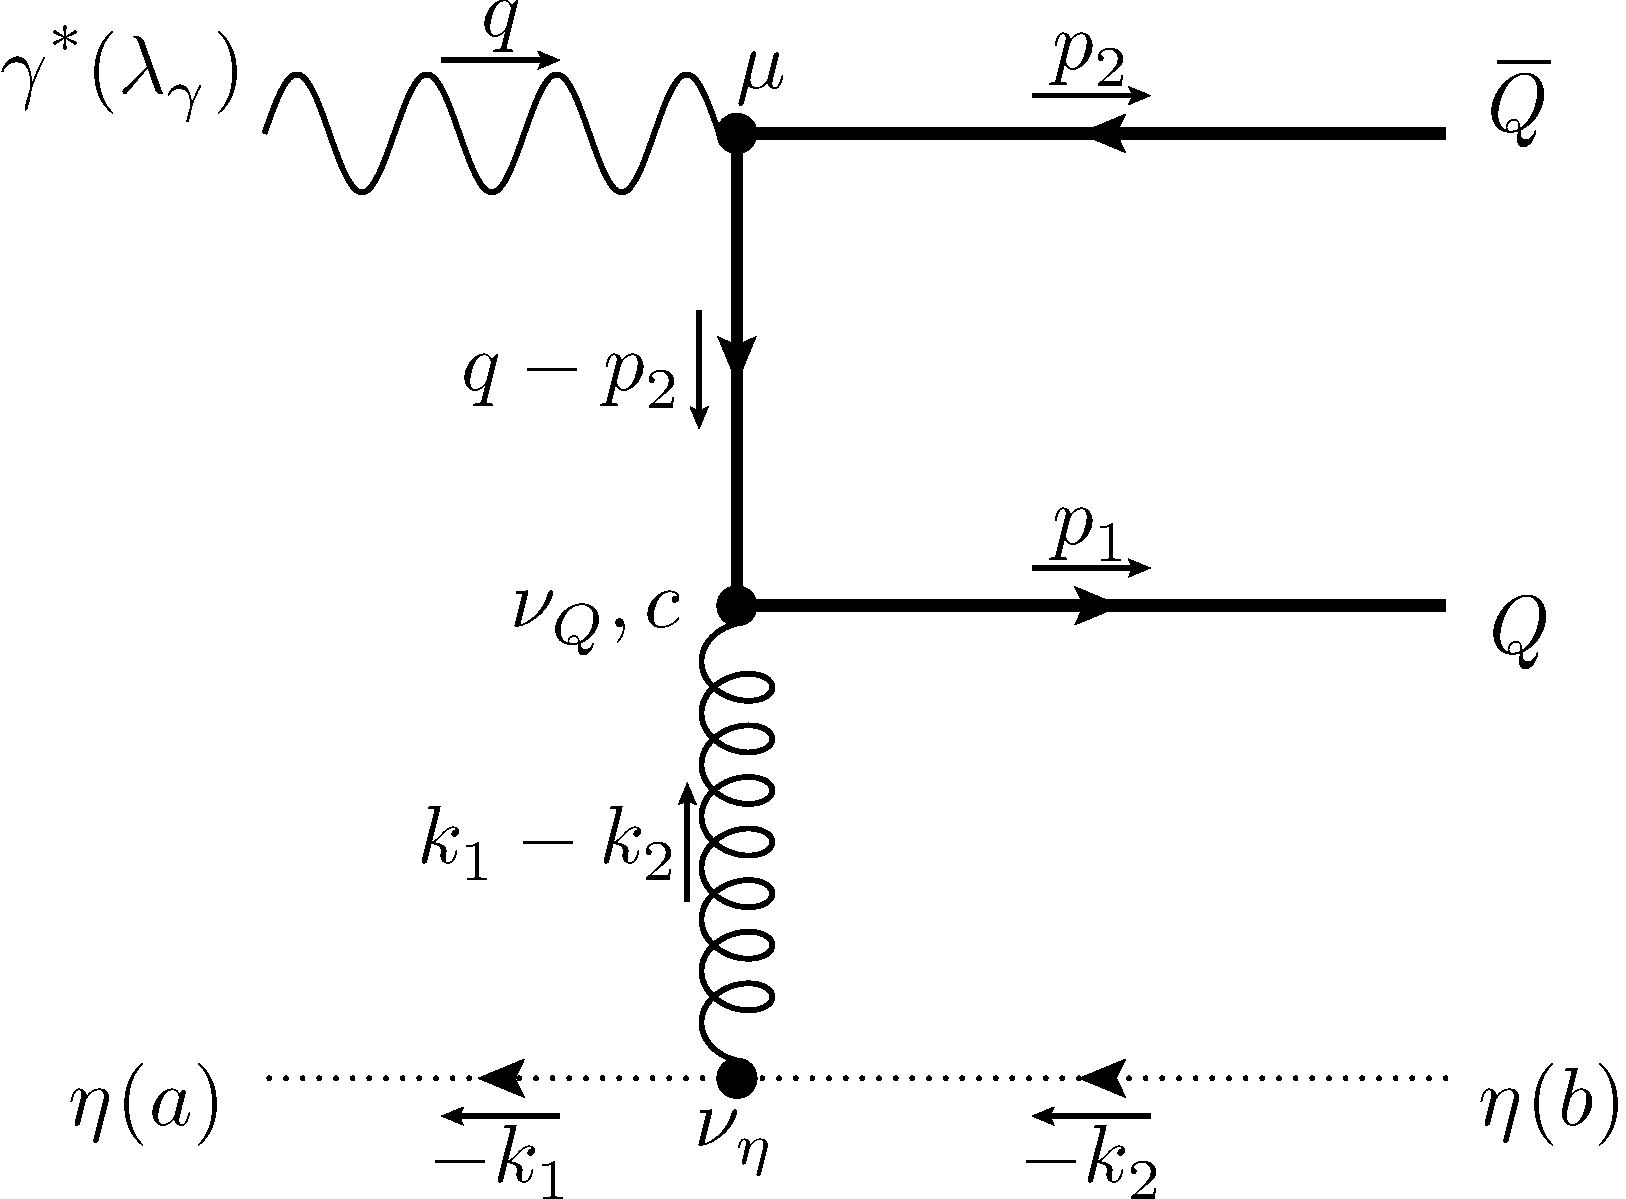
\includegraphics[width=\textwidth]{pyfeyn/nlo-gh-3}
		\caption{$i\Md^{(NLO,\Pgh)}_{3,\mu}$}
	\end{subfigure}\hspace{.1\textwidth}%
	\begin{subfigure}[t]{.42\textwidth}
		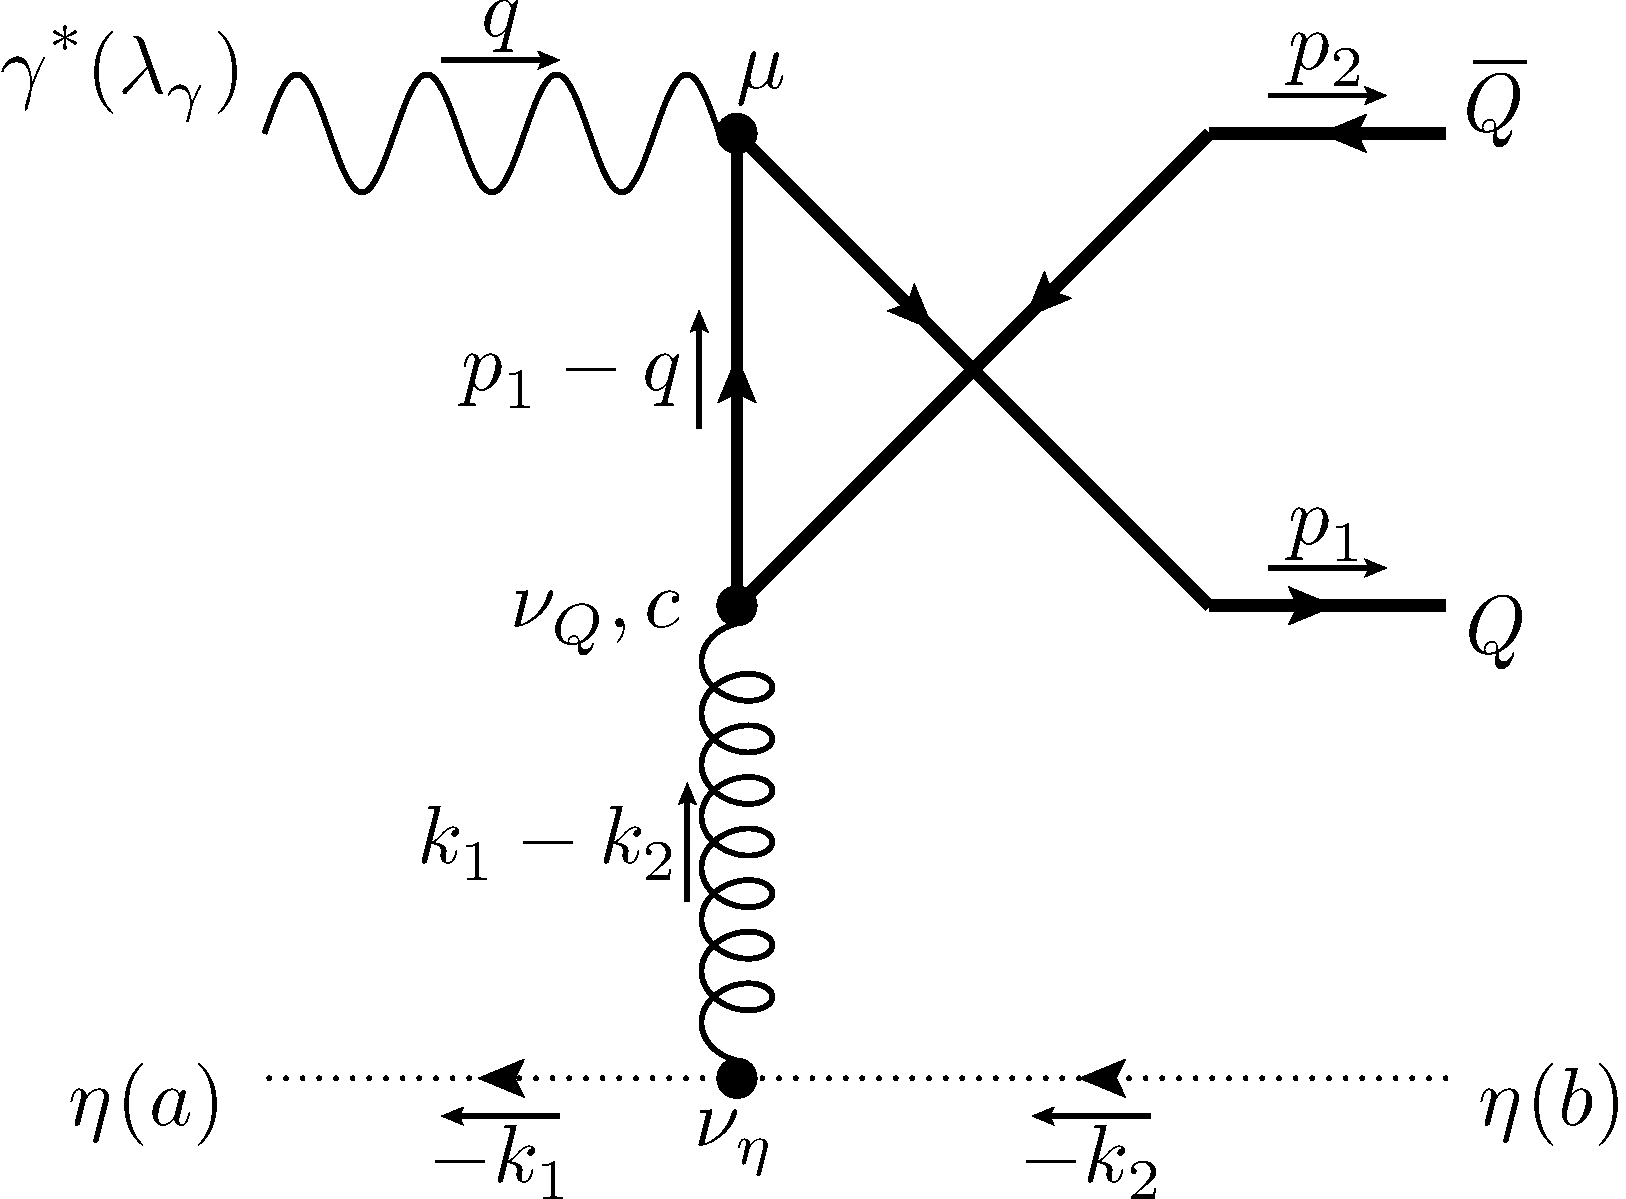
\includegraphics[width=\textwidth]{pyfeyn/nlo-gh-4}
		\caption{$i\Md^{(NLO,\Pgh)}_{4,\mu}$}
	\end{subfigure}
	\caption{NLO contributions by ghosts}\label{fig:FeynNLOgh}
\end{figure}

formula:
\begin{align}
i\Md^{(NLO,\Pgh)}_{1,\mu} &= \bar u(p_1)( igT_c\gamma^{\nu_Q})\frac{i(\slashed{q}-\slashed{p}_2+m)}{u_1}(-i e e_H \gamma_\mu) v(p_2)\cdot\frac{-g_{\nu_Q,\nu_{\Pgh}}}{t'} \cdot (gf^{acb}k_2^{\nu_{\Pgh}})\\
i\Md^{(NLO,\Pgh)}_{2,\mu} &= \bar u(p_1)(-i e e_H \gamma_\mu) \frac{i(\slashed{p}_1-\slashed{q}+m)}{u_7}( igT_c\gamma^{\nu_Q})v(p_2)\cdot\frac{-g_{\nu_Q,\nu_{\Pgh}}}{t'} \cdot (gf^{acb}k_2^{\nu_{\Pgh}})\\
i\Md^{(NLO,\Pgh)}_{3,\mu} &= \bar u(p_1)( igT_c\gamma^{\nu_Q})\frac{i(\slashed{q}-\slashed{p}_2+m)}{u_1}(-i e e_H \gamma_\mu) v(p_2)\cdot\frac{-g_{\nu_Q,\nu_{\Pgh}}}{t'} \cdot (gf^{cab}(-k_1)^{\nu_{\Pgh}})\\
i\Md^{(NLO,\Pgh)}_{4,\mu} &= \bar u(p_1)(-i e e_H \gamma_\mu) \frac{i(\slashed{p}_1-\slashed{q}+m)}{u_7}( igT_c\gamma^{\nu_Q})v(p_2)\cdot\frac{-g_{\nu_Q,\nu_{\Pgh}}}{t'} \cdot (gf^{cab}(-k_1)^{\nu_{\Pgh}})
\end{align}

color space:
\begin{align}
\abs{\Md^{(NLO,\Pgh)}_{1,\mu}+\Md^{(NLO,\Pgh)}_{2,\mu}}^2 &\sim f_{acb}f_{adb}\tr(T_cT_d) = N_C C_F C_A\\
\abs{\Md^{(NLO,\Pgh)}_{3,\mu}+\Md^{(NLO,\Pgh)}_{4,\mu}}^2 &\sim f_{cab}f_{dab}\tr(T_c T_d) = f_{acb}f_{adb}\tr(T_cT_d) = N_C C_F C_A
\end{align}


\subsection{Virtual Contributions}
\begin{equation}
\Pggx(q) + \Pg(k_1) \rightarrow \PaQ(p_2) + \PQ(p_1)
\end{equation}

\begin{figure}[ht!]
	\centering
	\begin{subfigure}[t]{.4\textwidth}
		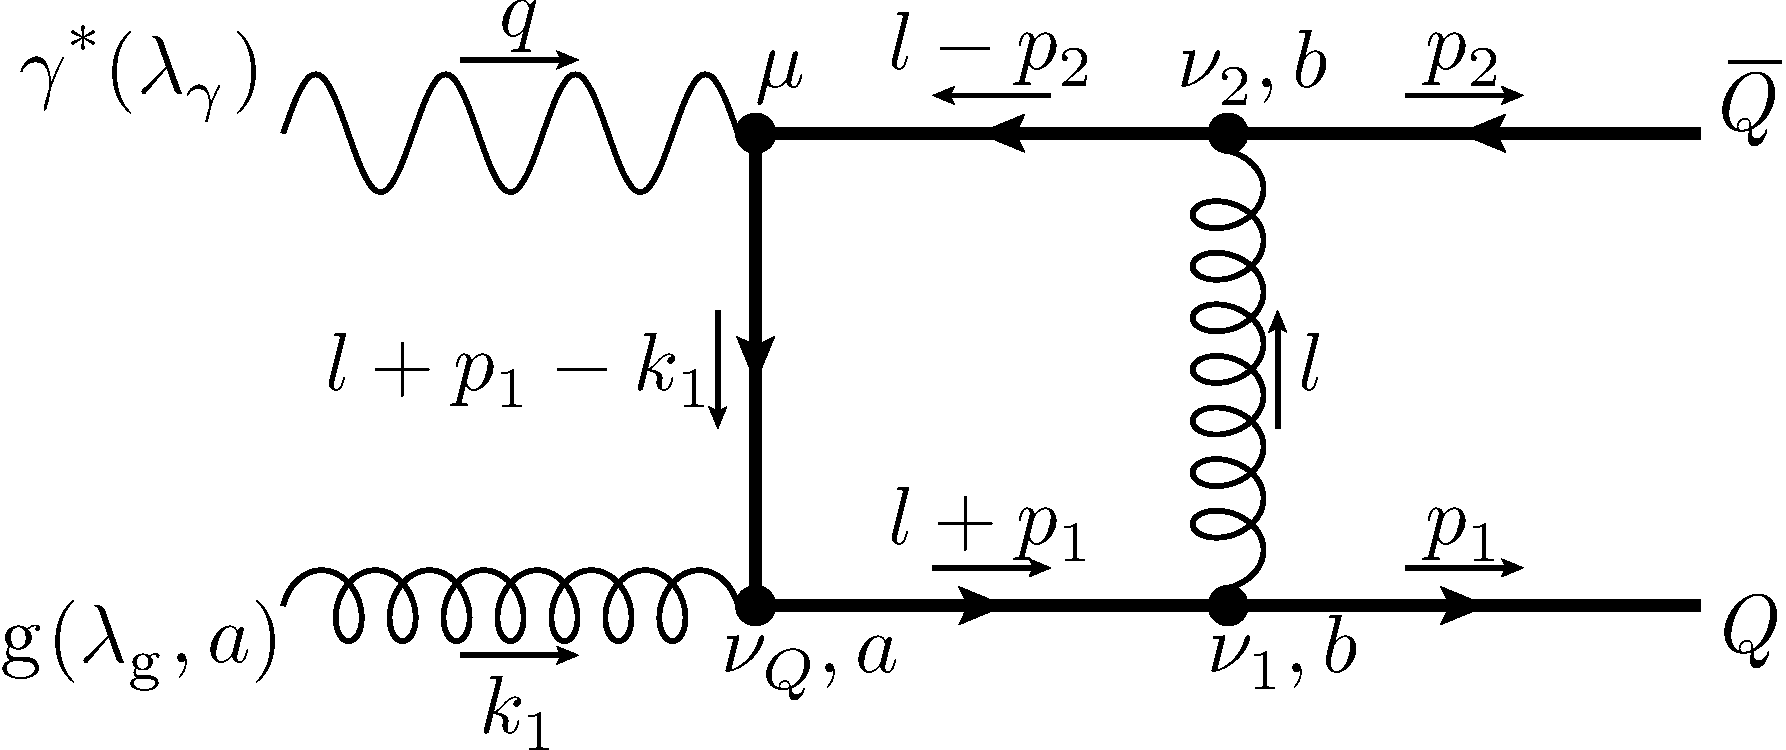
\includegraphics[width=\textwidth]{pyfeyn/nlo-v-box1}
		\caption{$i\Md^{(NLO,v)}_{1,\mu}$}
	\end{subfigure}\hspace{.15\textwidth}%
	\begin{subfigure}[t]{.4\textwidth}
		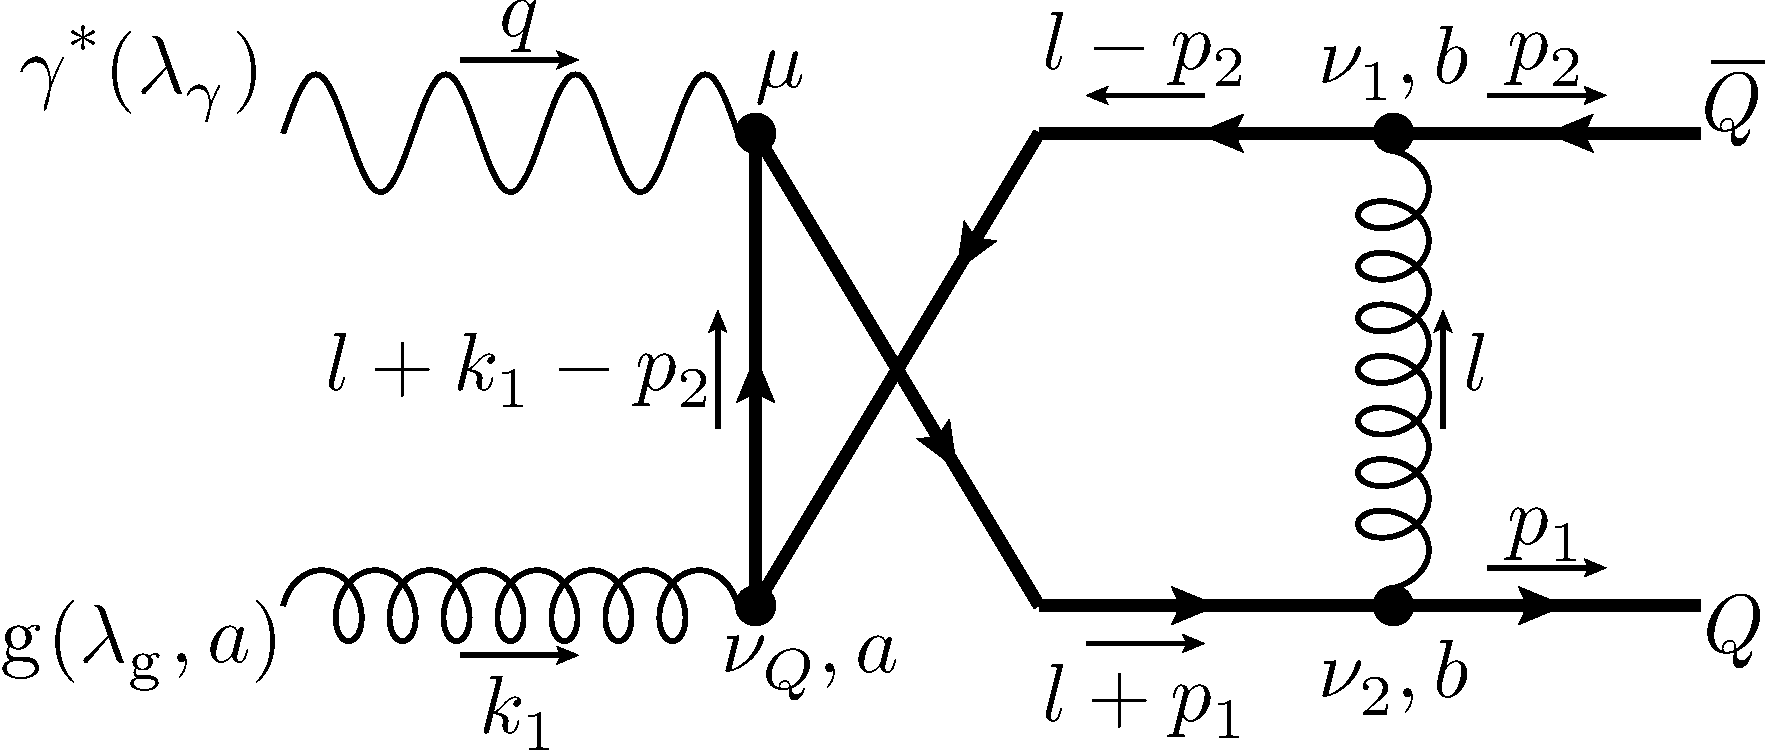
\includegraphics[width=\textwidth]{pyfeyn/nlo-v-box1cr}
		\caption{$i\Md^{(NLO,v)}_{2,\mu}$}
	\end{subfigure}\\
	\begin{subfigure}[t]{.6\textwidth}
		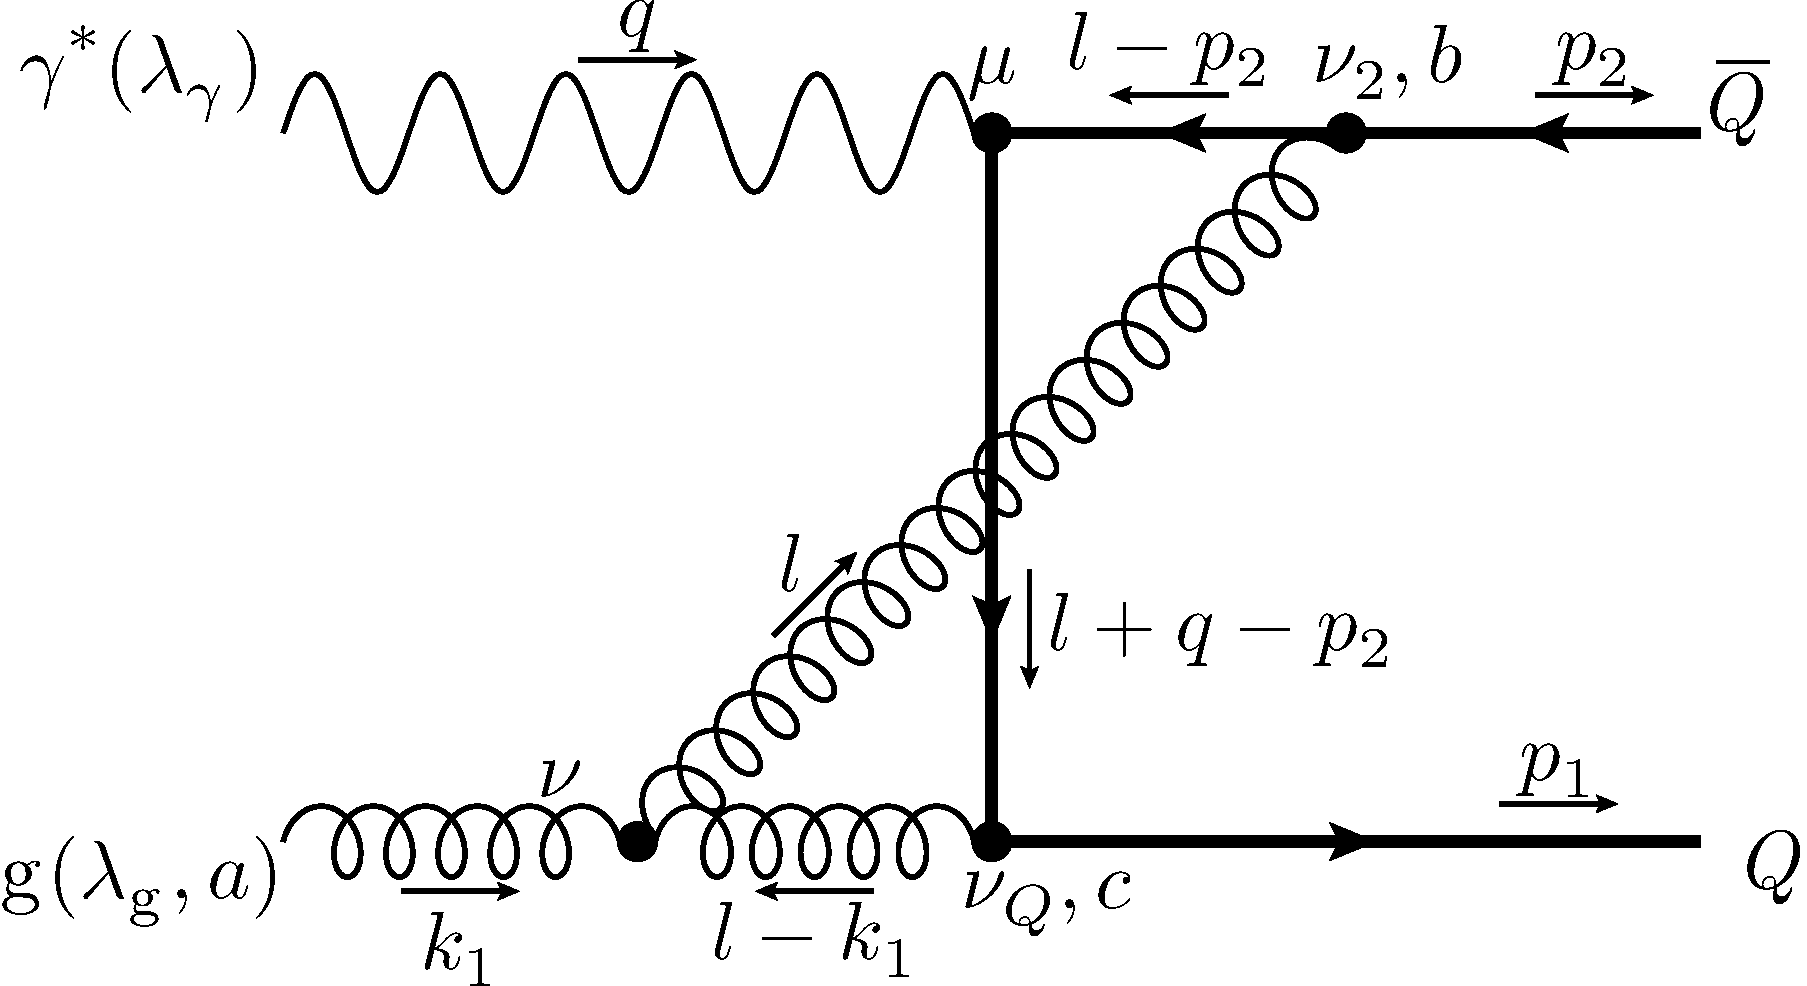
\includegraphics[width=\textwidth]{pyfeyn/nlo-v-box2}
		\caption{$i\Md^{(NLO,v)}_{3,\mu}$}
	\end{subfigure}
	\caption{NLO contributions by one loop}\label{fig:FeynNLOvab}
\end{figure}

\begin{align}
i\Md^{(NLO,v)}_{1,\mu} &=\mu_R^{4-n}\!\!\int\!\!\frac{d^nl}{(2\pi)^n}\,\bar u(p_1)(igT_b\gamma^{\nu_1})\frac{i(\slashed{l}+\slashed{p}_1+m)}{(l+p_1)^2-m^2}(igT_a\gamma^{\nu_Q})\frac{i(\slashed{l}+\slashed{p}_1-\slashed{k}_1+m)}{(l+p_1-k_1)^2-m^2}\cdot\nonumber\\
 &\hspace{40pt}(-i e e_H \gamma_\mu)\frac{i(\slashed{l}-\slashed{p}_2+m)}{(l-p_2)^2-m^2}(igT_b\gamma^{\nu_2})\frac{-ig_{\nu_1,\nu_2}}{l^2}v(p_2)\varepsilon^{(\lambda_{\Pg})}_{\nu_Q}(k_1)\\
i\Md^{(NLO,v)}_{2,\mu} &= \mu_R^{4-n}\!\!\int\!\!\frac{d^nl}{(2\pi)^n}\,\bar u(p_1)(igT_b\gamma^{\nu_1})\frac{i(\slashed{l}+\slashed{p}_1+m)}{(l+p_1)^2-m^2}(igT_a\gamma^{\nu_Q})\frac{i(\slashed{l}+\slashed{p}_1-\slashed{q}+m)}{(l+p_1-q)^2-m^2}\cdot\nonumber\\
 &\hspace{40pt}(-i e e_H \gamma_\mu)\frac{i(\slashed{l}-\slashed{p}_2+m)}{(l-p_2)^2-m^2}(igT_b\gamma^{\nu_2})\frac{-ig_{\nu_1,\nu_2}}{l^2}v(p_2)\varepsilon^{(\lambda_{\Pg})}_{\nu_Q}(k_1)\\
i\Md^{(NLO,v)}_{3,\mu} &=\mu_R^{4-n}\!\!\int\!\!\frac{d^nl}{(2\pi)^n}\,\bar u(p_1)(igT_c\gamma^{\nu_Q})\frac{i(\slashed{l}+\slashed{q}_1-\slashed{p}_2+m)}{(l+q-p_2)^2-m^2}(-i e e_H \gamma_\mu)\frac{i(\slashed{l}-\slashed{p}_2+m)}{(l-p_2)^2-m^2}\cdot\nonumber\\
 &\hspace{20pt}(igT_b\gamma^{\nu_2})\frac{(-i)^2}{l^2(l-k_1)^2}v(p_2)\varepsilon^{\nu,(\lambda_{\Pg})}(k_1)\cdot\nonumber\\
 &\hspace{20pt}\left(gf_{abc}\left(g_{\nu_2\nu_Q}(k_1-2l)_\nu+g_{\nu_Q\nu}(l-2k_1)_{\nu_2}+g_{\nu\nu_2}(k_1+l)_{\nu_Q}\right)\right)
\end{align}

\pagebreak

\begin{figure}[ht!]
	\begin{subfigure}[t]{.4\textwidth}
		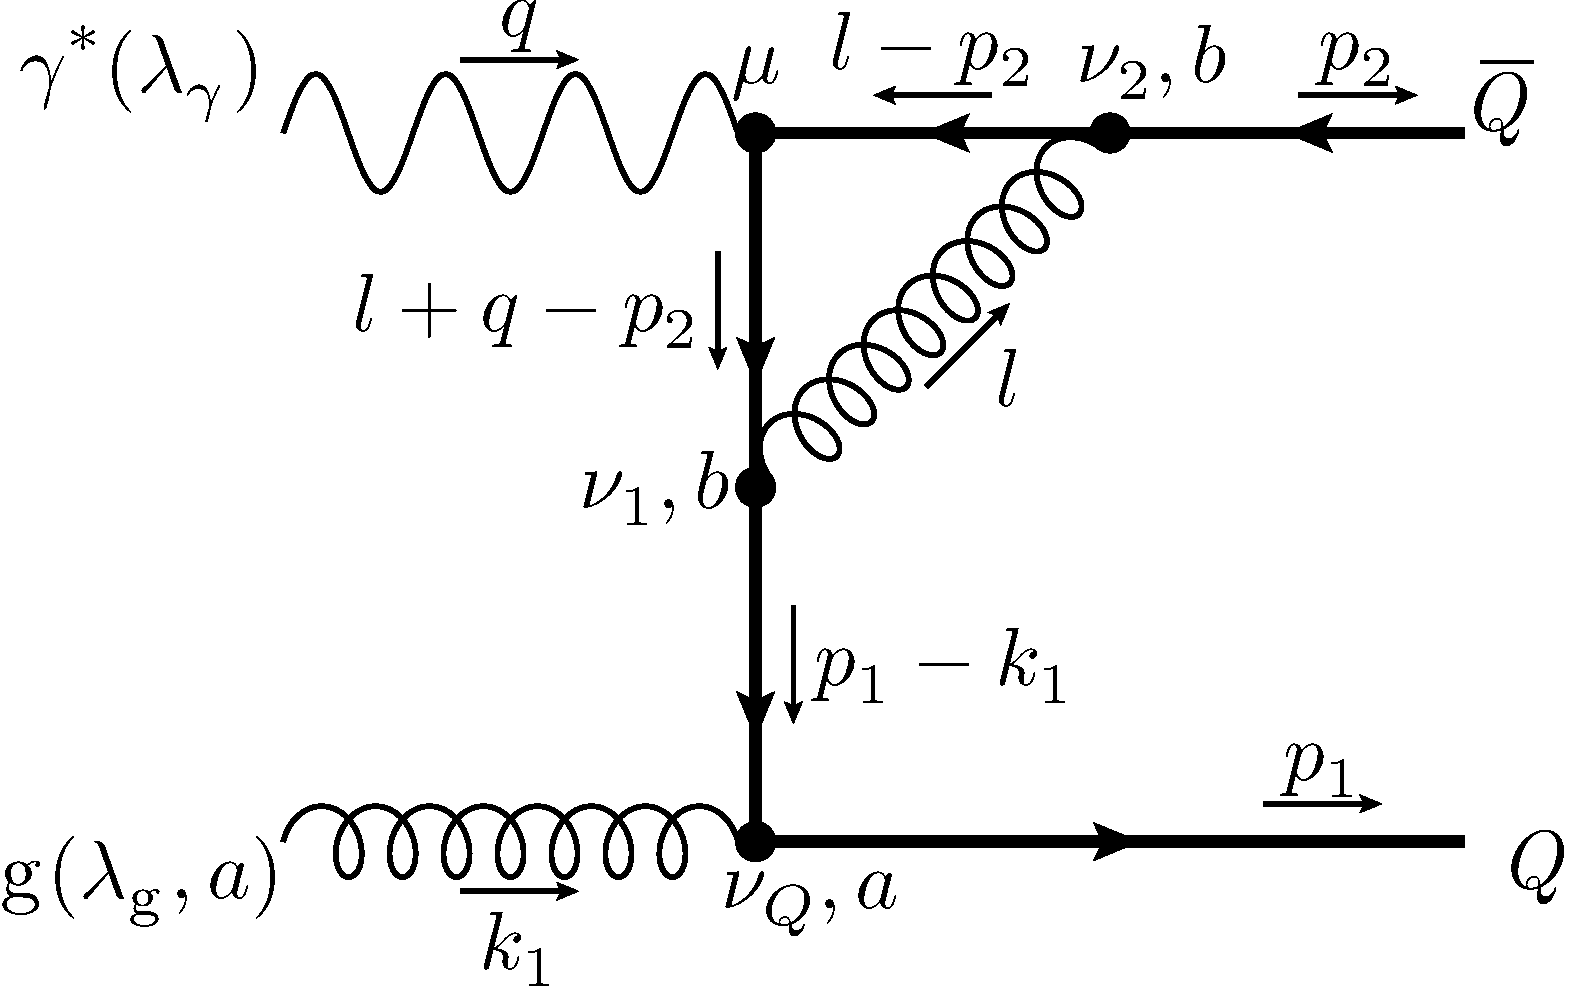
\includegraphics[width=\textwidth]{pyfeyn/nlo-v-e}
		\caption{$i\Md^{(NLO,v)}_{5,\mu}$}
	\end{subfigure}\hspace{.15\textwidth}%
	\begin{subfigure}[t]{.4\textwidth}
		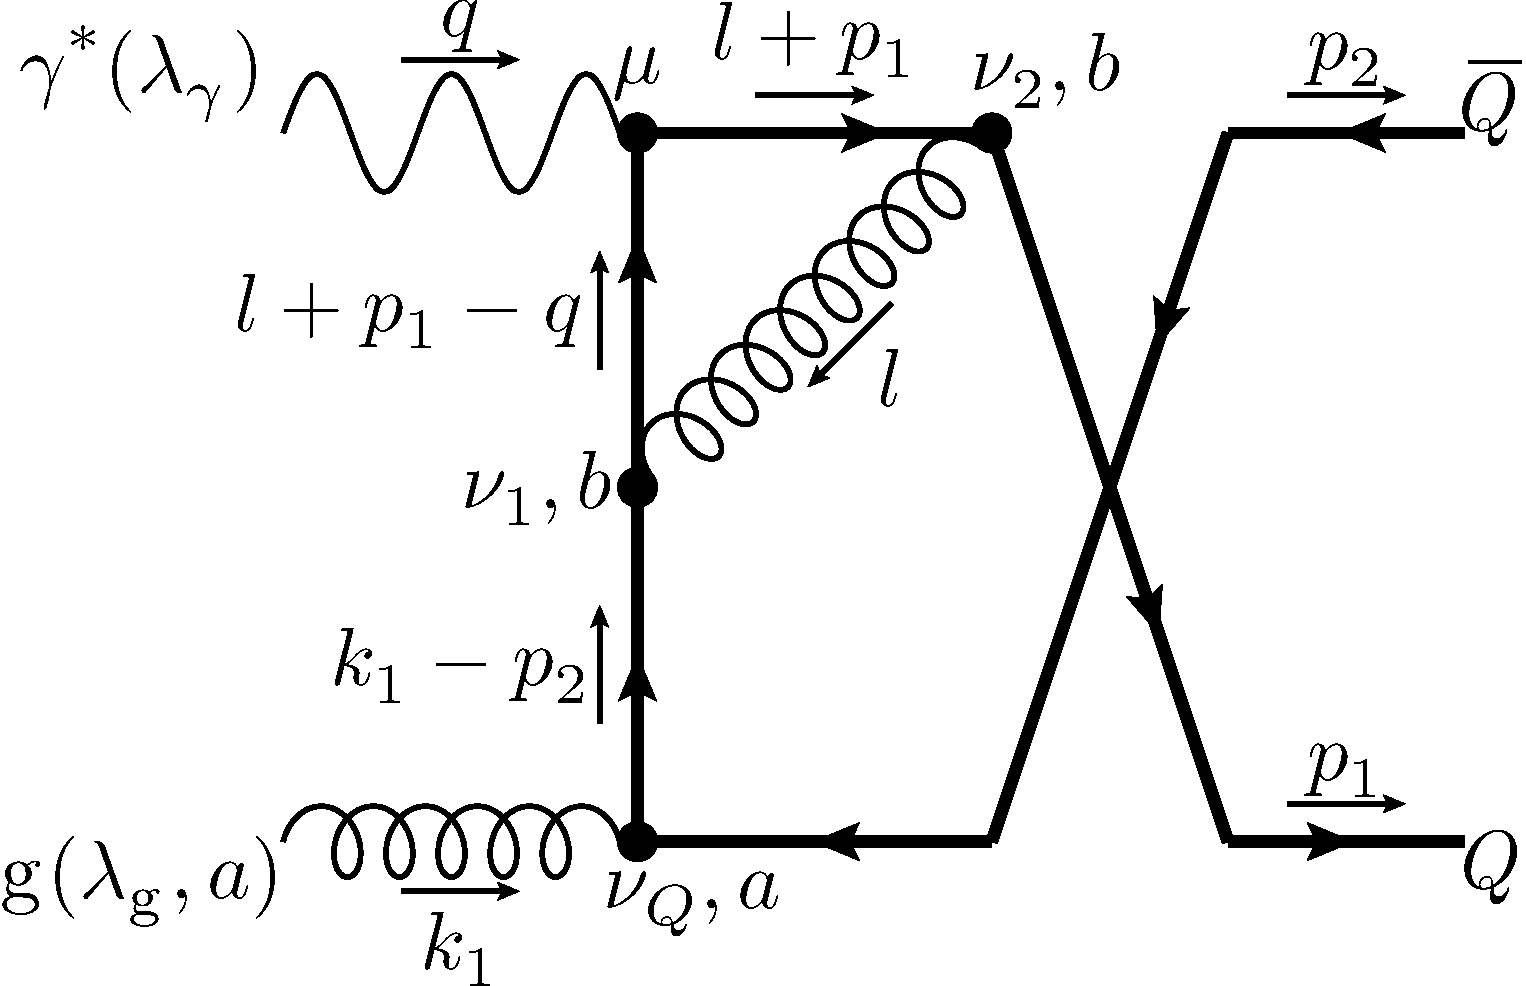
\includegraphics[width=\textwidth]{pyfeyn/nlo-v-ecr}
		\caption{$i\Md^{(NLO,v)}_{6,\mu}$}
	\end{subfigure}\\
	\begin{subfigure}[t]{.4\textwidth}
		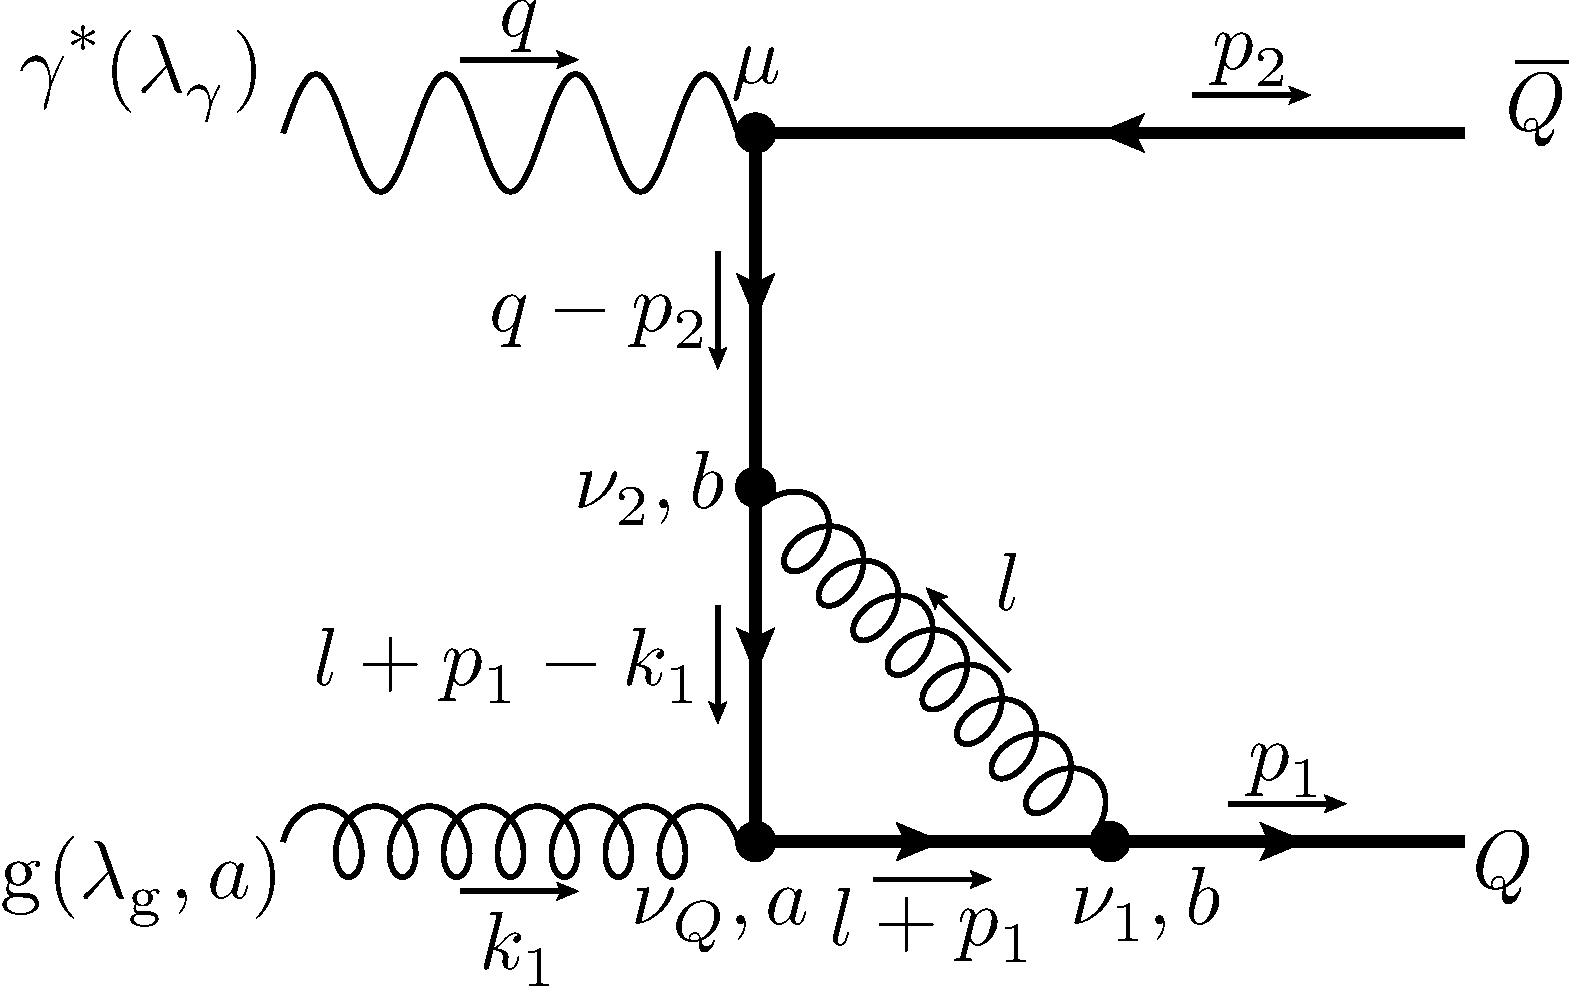
\includegraphics[width=\textwidth]{pyfeyn/nlo-v-g1}
		\caption{$i\Md^{(NLO,v)}_{7,\mu}$}
	\end{subfigure}\hspace{.15\textwidth}%
	\begin{subfigure}[t]{.4\textwidth}
		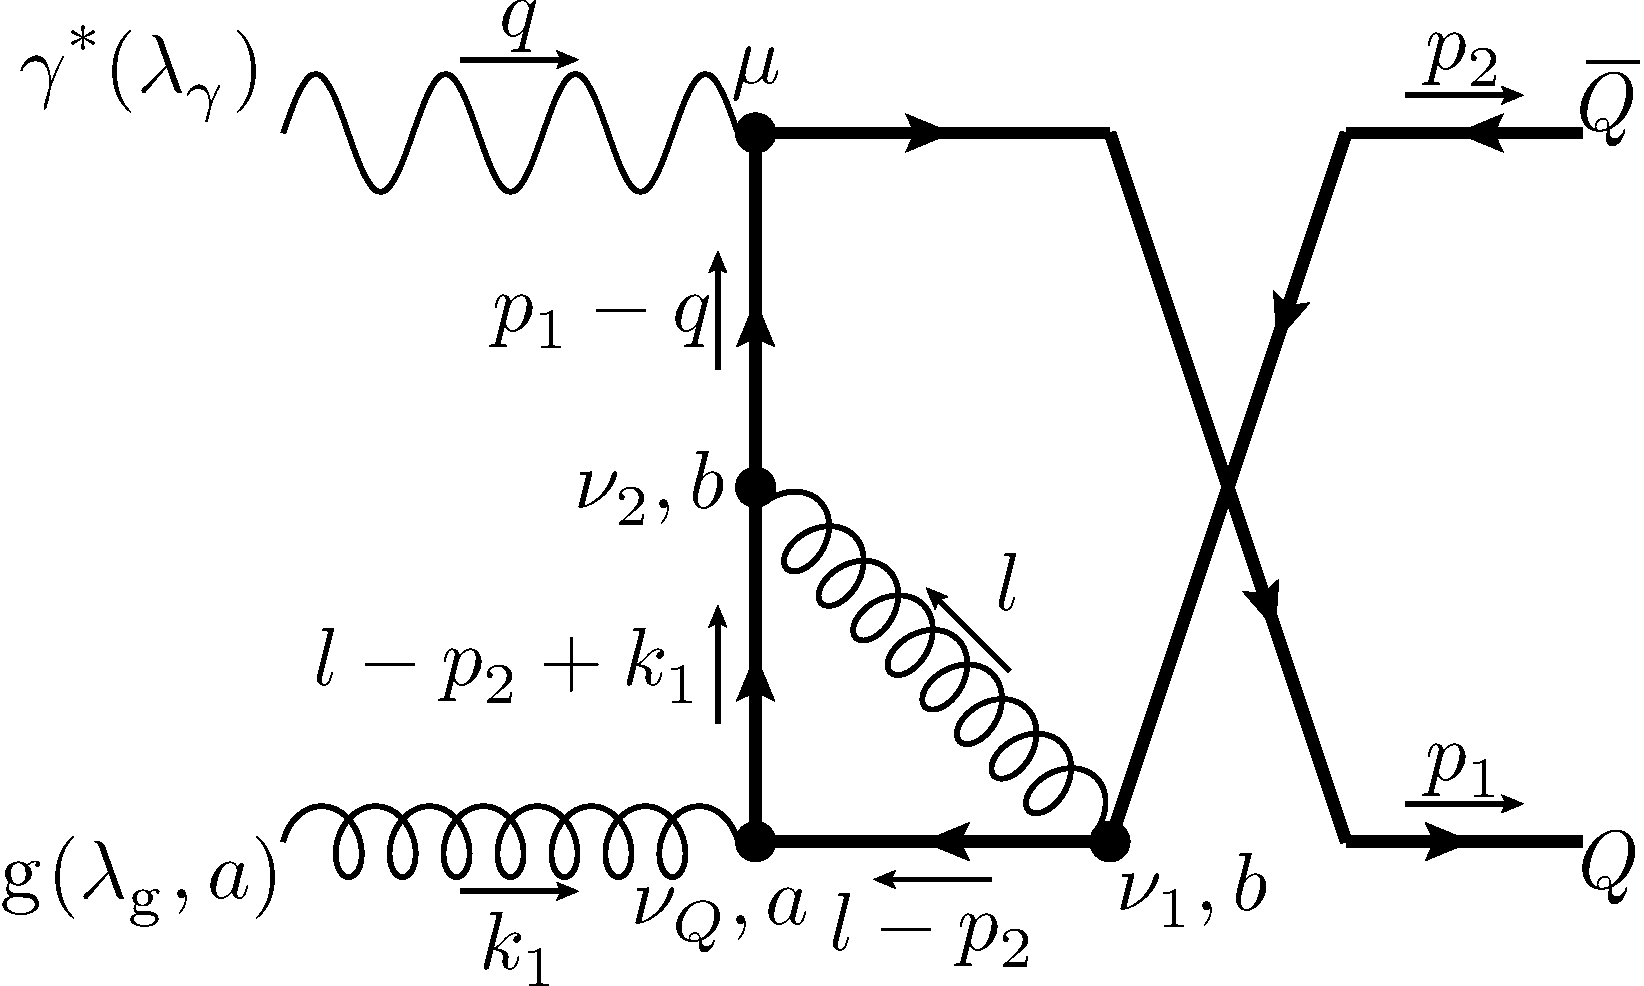
\includegraphics[width=\textwidth]{pyfeyn/nlo-v-g1cr}
		\caption{$i\Md^{(NLO,v)}_{8,\mu}$}
	\end{subfigure}
	\caption{NLO contributions by one loop (cont'ed)}\label{fig:FeynNLOvcd}
\end{figure}

\begin{align}
i\Md^{(NLO,v)}_{5,\mu} &=\mu_R^{4-n}\!\!\int\!\!\frac{d^nl}{(2\pi)^n}\,\bar u(p_1)(igT_a\gamma^{\nu_Q})\frac{i(\slashed{p}_1-\slashed{k}_1+m)}{u_1}(igT_b\gamma^{\nu_1})\frac{i(\slashed{l}+\slashed{q}-\slashed{p}_2+m)}{(l+q-p_2)^2-m^2}\cdot\nonumber\\
 &\hspace{40pt}(-i e e_H \gamma_\mu)\frac{i(\slashed{l}-\slashed{p}_2+m)}{(l-p_2)^2-m^2}(igT_b\gamma^{\nu_2})\frac{-ig_{\nu_1,\nu_2}}{l^2}v(p_2)\varepsilon^{(\lambda_{\Pg})}_{\nu_Q}(k_1)\\
i\Md^{(NLO,v)}_{6,\mu} &=\mu_R^{4-n}\!\!\int\!\!\frac{d^nl}{(2\pi)^n}\,\bar u(p_1)(igT_b\gamma^{\nu_2})\frac{i(\slashed{l}+\slashed{p}_1+m)}{(l+p_1)^2-m^2}(-i e e_H \gamma_\mu)\frac{i(\slashed{l}+\slashed{p}_1-\slashed{q}+m)}{(l+p_1-q)^2-m^2}\cdot\nonumber\\
 &\hspace{40pt}(igT_b\gamma^{\nu_1})\frac{i(\slashed{k}_1-\slashed{p}_2+m)}{t_1}(igT_a\gamma^{\nu_Q})\frac{-ig_{\nu_1,\nu_2}}{l^2}v(p_2)\varepsilon^{(\lambda_{\Pg})}_{\nu_Q}(k_1)\\
i\Md^{(NLO,v)}_{7,\mu} &=\mu_R^{4-n}\!\!\int\!\!\frac{d^nl}{(2\pi)^n}\,\bar u(p_1)(igT_b\gamma^{\nu_1})\frac{i(\slashed{l}+\slashed{p}_1+m)}{(l+p_1)^2-m^2}(igT_a\gamma^{\nu_Q})\frac{i(\slashed{l}+\slashed{p}_1-\slashed{k}_1+m)}{(l+p_1-k_1)^2-m^2}\cdot\nonumber\\
 &\hspace{40pt}(igT_b\gamma^{\nu_2})\frac{i(\slashed{q}-\slashed{p}_2+m)}{u_1}(-i e e_H \gamma_\mu)\frac{-ig_{\nu_1,\nu_2}}{l^2}v(p_2)\varepsilon^{(\lambda_{\Pg})}_{\nu_Q}(k_1)\\
i\Md^{(NLO,v)}_{8,\mu} &=\mu_R^{4-n}\!\!\int\!\!\frac{d^nl}{(2\pi)^n}\,\bar u(p_1)(-i e e_H \gamma_\mu)\frac{i(\slashed{p}_1-\slashed{q}+m)}{t_1}(igT_b\gamma^{\nu_2})\frac{i(\slashed{l}-\slashed{p}_2+\slashed{k}_1+m)}{(l-p_2+k_1)^2-m^2}\cdot\nonumber\\
 &\hspace{40pt}(igT_a\gamma^{\nu_Q})\frac{i(\slashed{l}-\slashed{p}_2+m)}{(l-p_2)^2-m^2}(igT_b\gamma^{\nu_1})\frac{-ig_{\nu_1,\nu_2}}{l^2}v(p_2)\varepsilon^{(\lambda_{\Pg})}_{\nu_Q}(k_1)
\end{align}

\pagebreak

\begin{figure}[ht!]
	\begin{subfigure}[t]{.4\textwidth}
		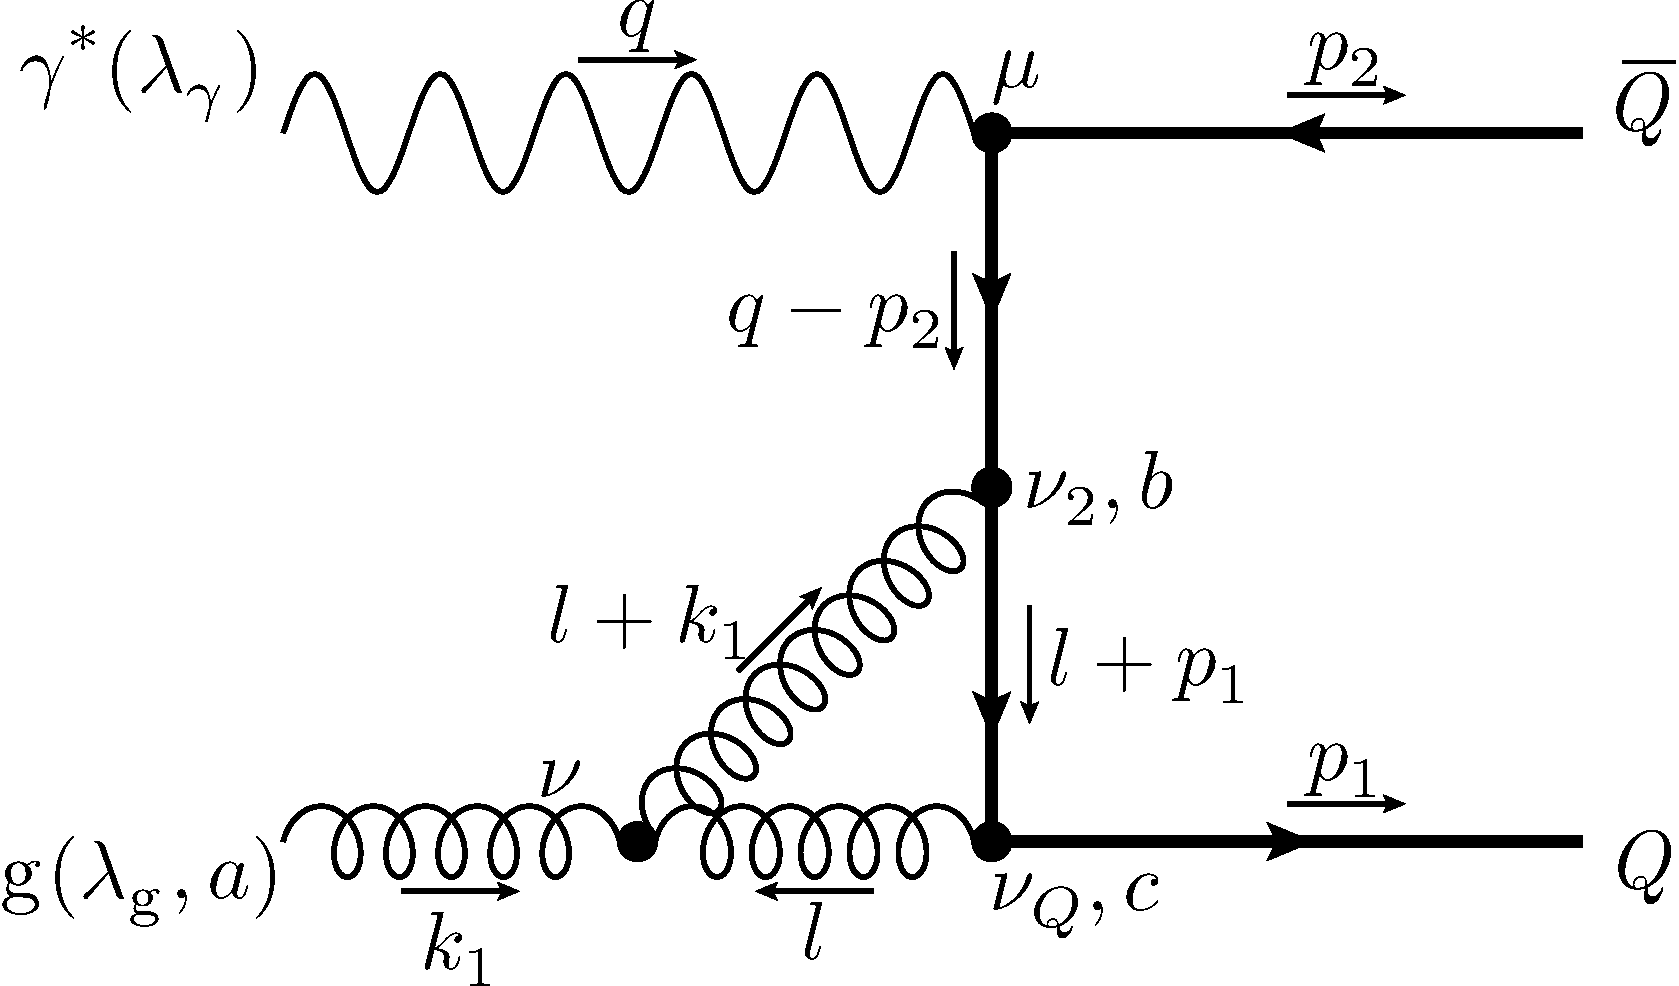
\includegraphics[width=\textwidth]{pyfeyn/nlo-v-g2}
		\caption{$i\Md^{(NLO,v)}_{9,\mu}$}
	\end{subfigure}\hspace{.15\textwidth}%
	\begin{subfigure}[t]{.4\textwidth}
		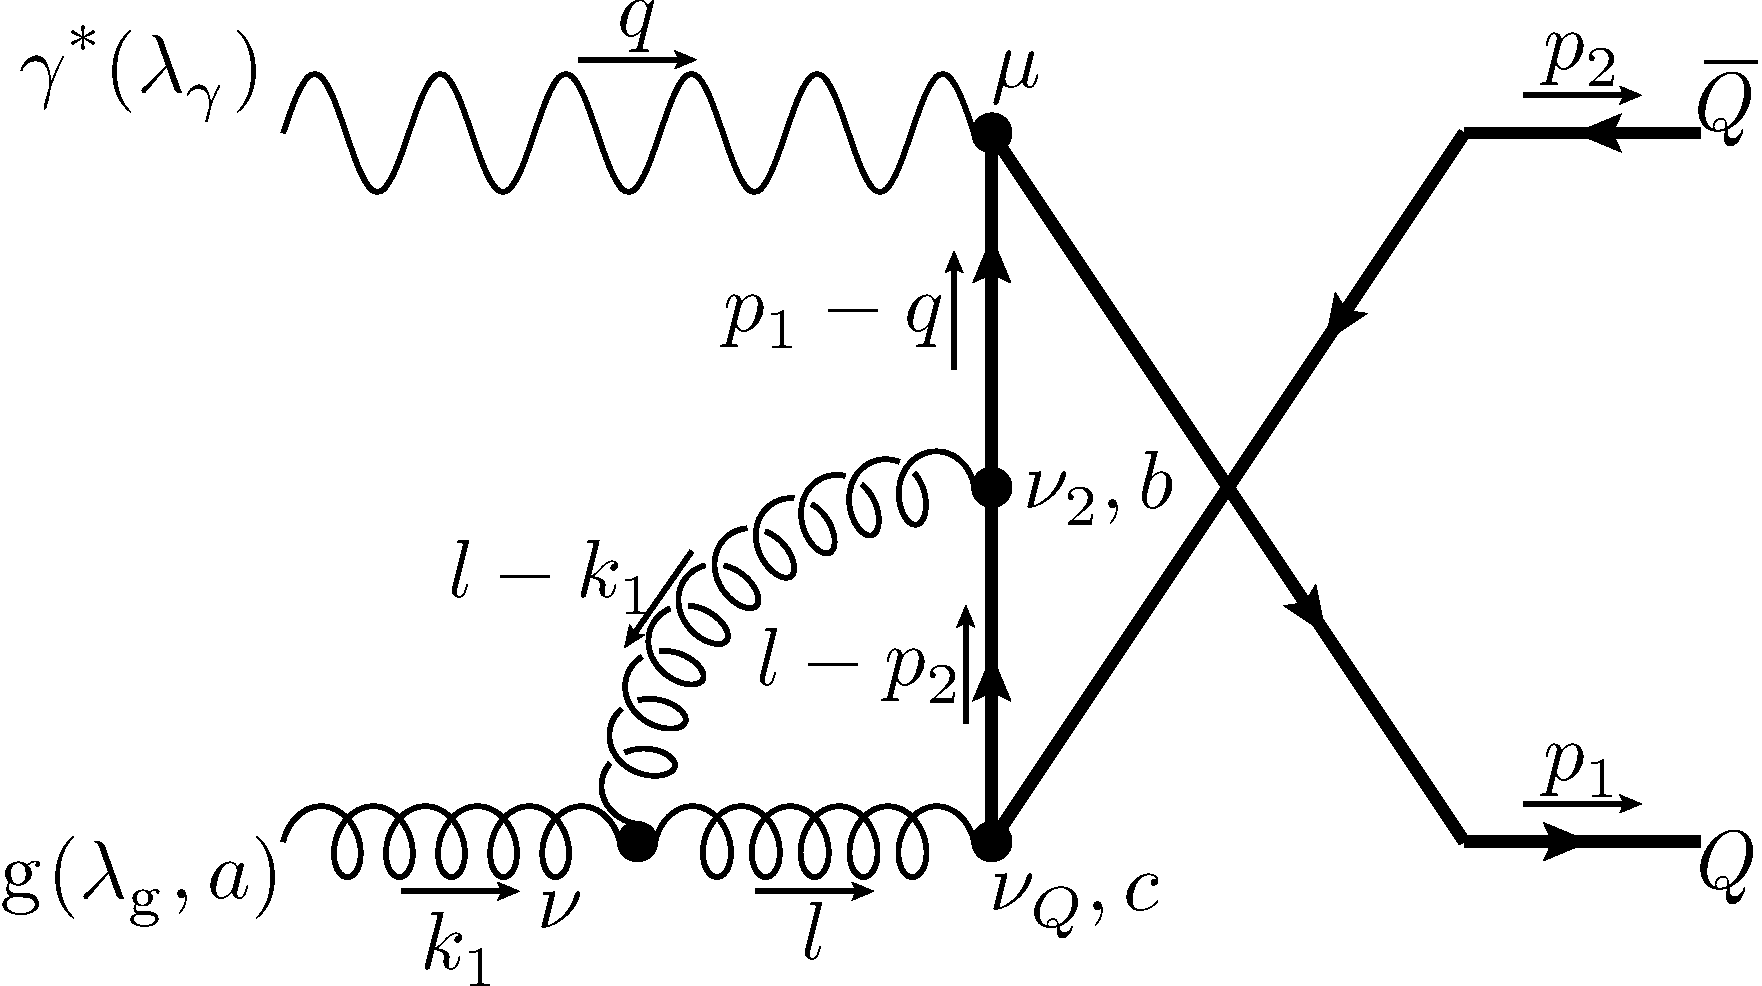
\includegraphics[width=\textwidth]{pyfeyn/nlo-v-g2cr}
		\caption{$i\Md^{(NLO,v)}_{10,\mu}$}
	\end{subfigure}\\
	\begin{subfigure}[t]{.4\textwidth}
		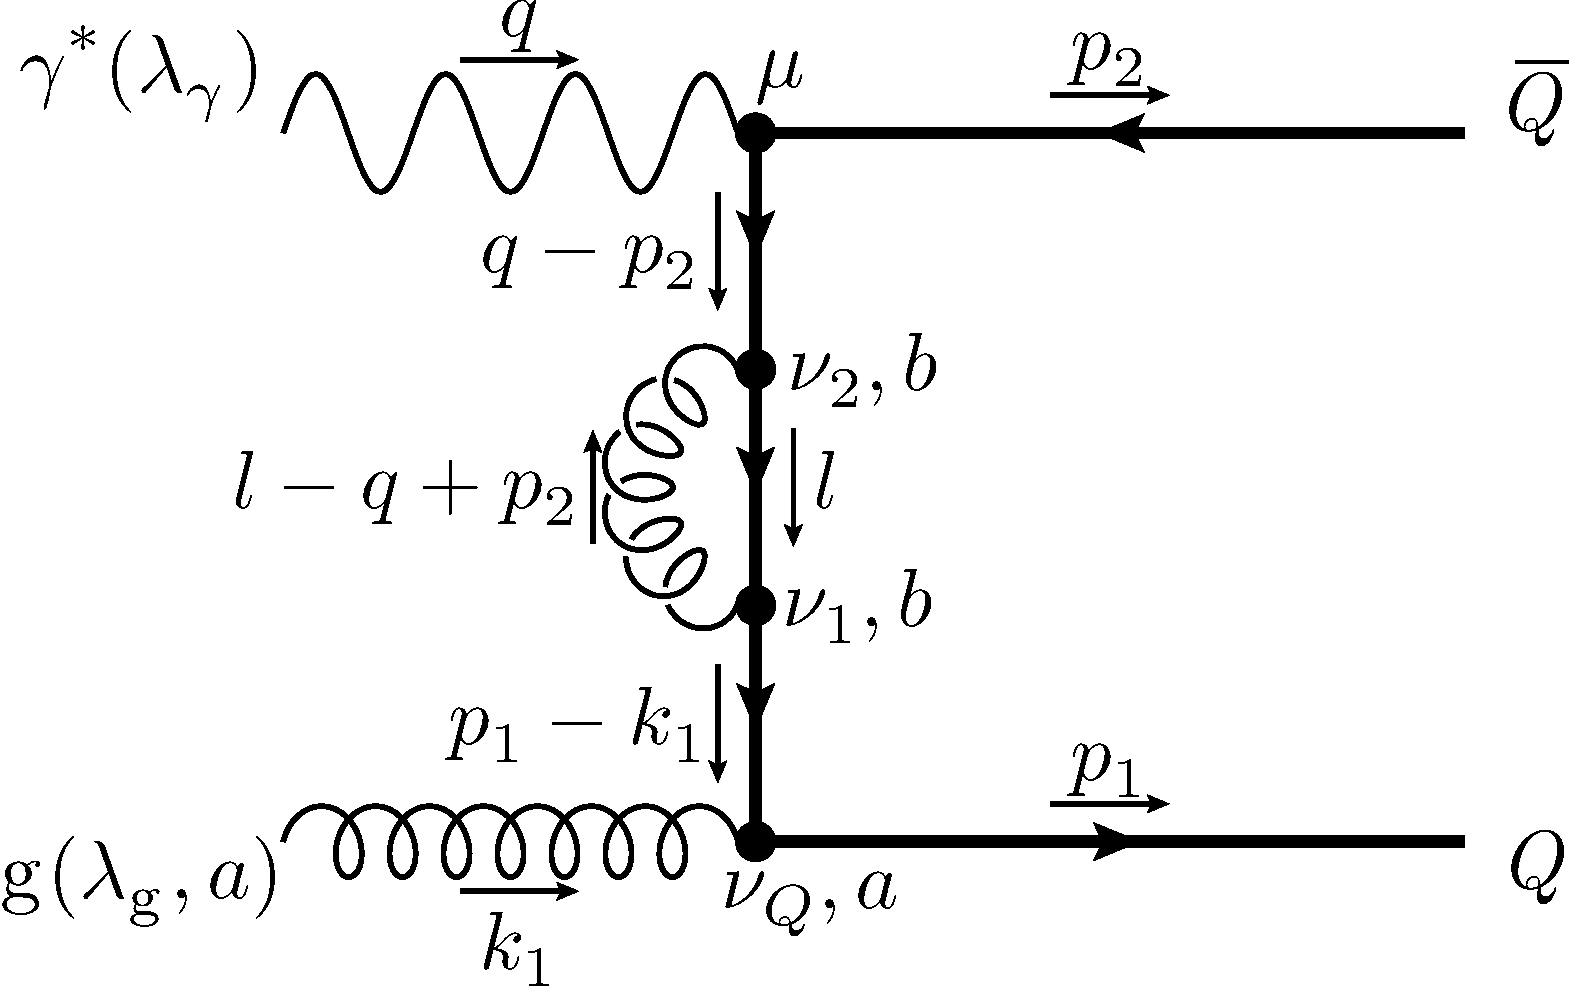
\includegraphics[width=\textwidth]{pyfeyn/nlo-v-m1}
		\caption{$i\Md^{(NLO,v)}_{11,\mu}$}
	\end{subfigure}\hspace{.15\textwidth}%
	\begin{subfigure}[t]{.4\textwidth}
		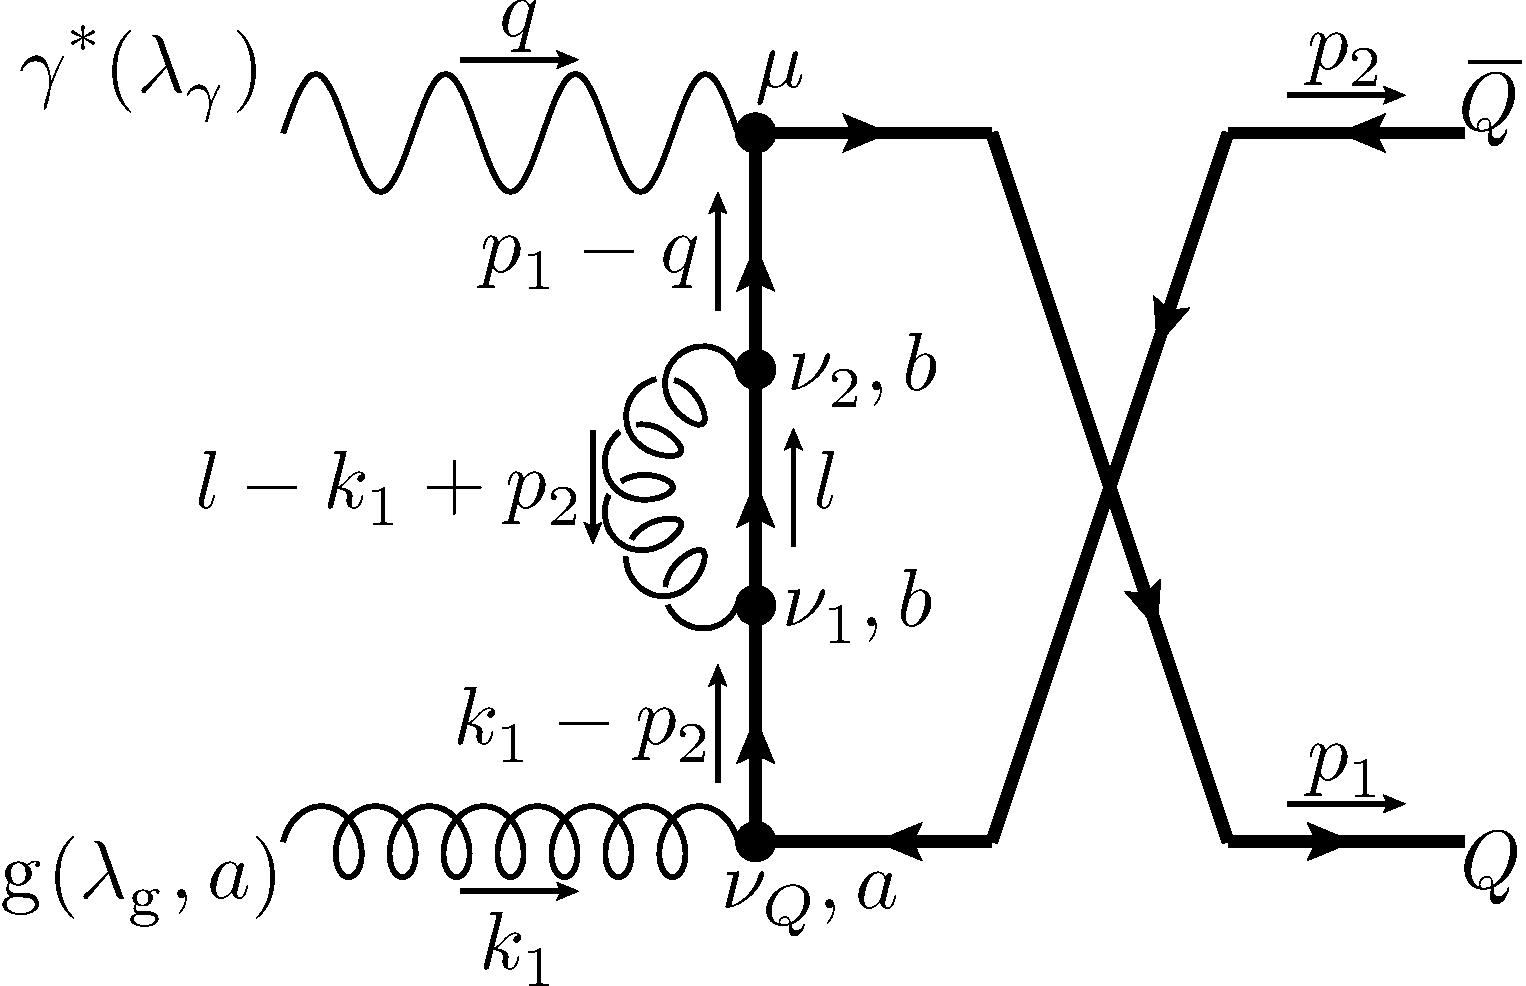
\includegraphics[width=\textwidth]{pyfeyn/nlo-v-m1cr}
		\caption{$i\Md^{(NLO,v)}_{12,\mu}$}
	\end{subfigure}
	\caption{NLO contributions by one loop (cont'ed)}\label{fig:FeynNLOve}
\end{figure}

\begin{align}
i\Md^{(NLO,v)}_{9,\mu} &=\mu_R^{4-n}\!\!\int\!\!\frac{d^nl}{(2\pi)^n}\,\bar u(p_1)(igT_c\gamma^{\nu_Q})\frac{i(\slashed{l}+\slashed{p}_1+m)}{(l+p_1)^2-m^2}(igT_b\gamma^{\nu_2})\frac{i(\slashed{q}-\slashed{p}_2+m)}{u_1}\cdot\nonumber\\
 &\hspace{20pt}(-i e e_H \gamma_\mu)\frac{(-i)^2}{l^2(l+k_1)^2}v(p_2)\varepsilon^{\nu,(\lambda_{\Pg})}(k_1)\cdot\nonumber\\
 &\hspace{20pt}\left(gf_{abc}\left(g_{\nu\nu_2}(2k_1+l)_{\nu_Q}+g_{\nu_2\nu_Q}(-2l-k_1)_{\nu}+g_{\nu_Q\nu}(l-k_1)_{\nu_2}\right)\right)\\
i\Md^{(NLO,v)}_{10,\mu} &=\mu_R^{4-n}\!\!\int\!\!\frac{d^nl}{(2\pi)^n}\,\bar u(p_1)(-i e e_H \gamma_\mu)\frac{i(\slashed{p}_1-\slashed{q}+m)}{t_1}(igT_b\gamma^{\nu_2})\frac{i(\slashed{l}-\slashed{p}_2+m)}{(l-p_2)^2-m^2}\cdot\nonumber\\
 &\hspace{20pt}(igT_c\gamma^{\nu_Q})\frac{(-i)^2}{l^2(l-k_1)^2}v(p_2)\varepsilon^{\nu,(\lambda_{\Pg})}(k_1)\cdot\nonumber\\
 &\hspace{20pt}\left(gf_{abc}\left(g_{\nu\nu_2}(2k_1-l)_{\nu_Q}+g_{\nu_2\nu_Q}(2l-k_1)_{\nu}+g_{\nu_Q\nu}(-l-k_1)_{\nu_2}\right)\right)\\
i\Md^{(NLO,v)}_{11,\mu} &=\mu_R^{4-n}\!\!\int\!\!\frac{d^nl}{(2\pi)^n}\,\bar u(p_1)(igT_a\gamma^{\nu_Q})\frac{i(\slashed{p}_1-\slashed{k}_1+m)}{t_1}(igT_b\gamma^{\nu_1})\frac{i(\slashed{l}+m)}{l^2-m^2}\cdot\nonumber\\
 &\hspace{40pt}(igT_b\gamma^{\nu_2})\frac{i(\slashed{q}-\slashed{p}_2+m)}{t_1}(-i e e_H \gamma_\mu)\frac{-ig_{\nu_1,\nu_2}}{(l-q+p_2)^2}v(p_2)\varepsilon^{(\lambda_{\Pg})}_{\nu_Q}(k_1)\\
i\Md^{(NLO,v)}_{12,\mu} &=\mu^{4-n}\!\!\int\!\!\frac{d^nl}{(2\pi)^n}\,\bar u(p_1)(-i e e_H \gamma_\mu)\frac{i(\slashed{p}_1-\slashed{q}+m)}{u_1}(igT_b\gamma^{\nu_2})\frac{i(\slashed{l}+m)}{l^2-m^2}\cdot\nonumber\\
 &\hspace{40pt}(igT_b\gamma^{\nu_1})\frac{i(\slashed{k}_1-\slashed{p}_2+m)}{u_1}(igT_a\gamma^{\nu_Q})\frac{-ig_{\nu_1,\nu_2}}{(l-k_1+p_2)^2}v(p_2)\varepsilon^{(\lambda_{\Pg})}_{\nu_Q}(k_1)
\end{align}

\begin{figure}[ht!]
	\begin{subfigure}[t]{.4\textwidth}
		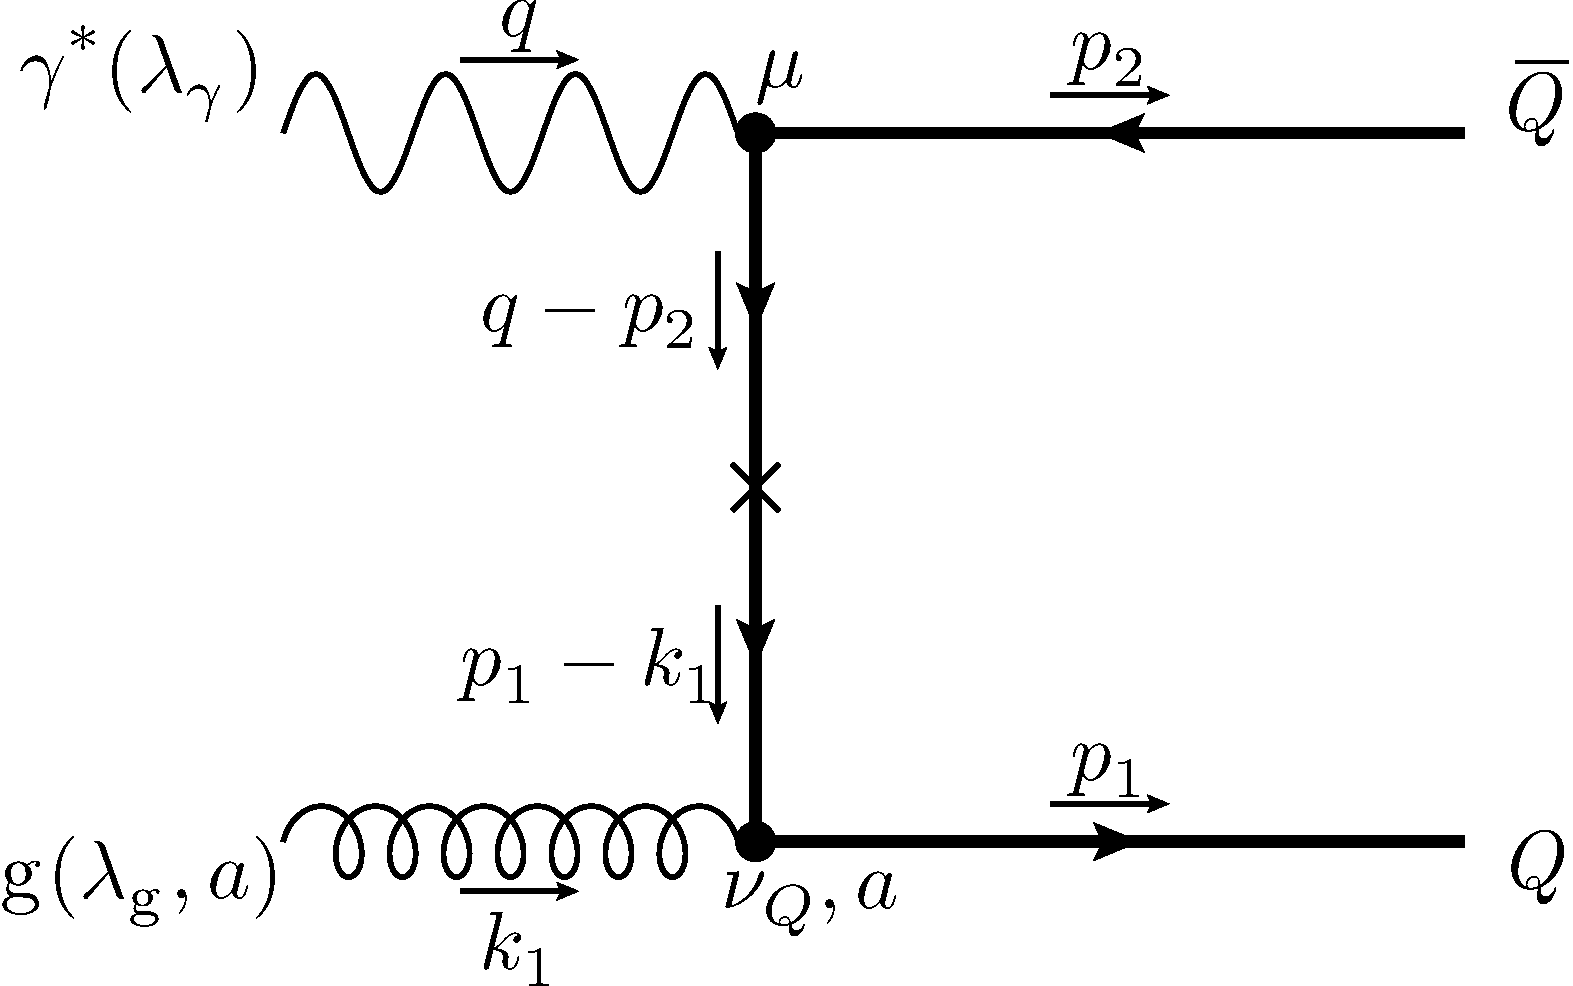
\includegraphics[width=\textwidth]{pyfeyn/nlo-c-m}
		\caption{$i\Md^{(NLO,c)}_{1,\mu}$}
	\end{subfigure}\hspace{.15\textwidth}%
	\begin{subfigure}[t]{.4\textwidth}
		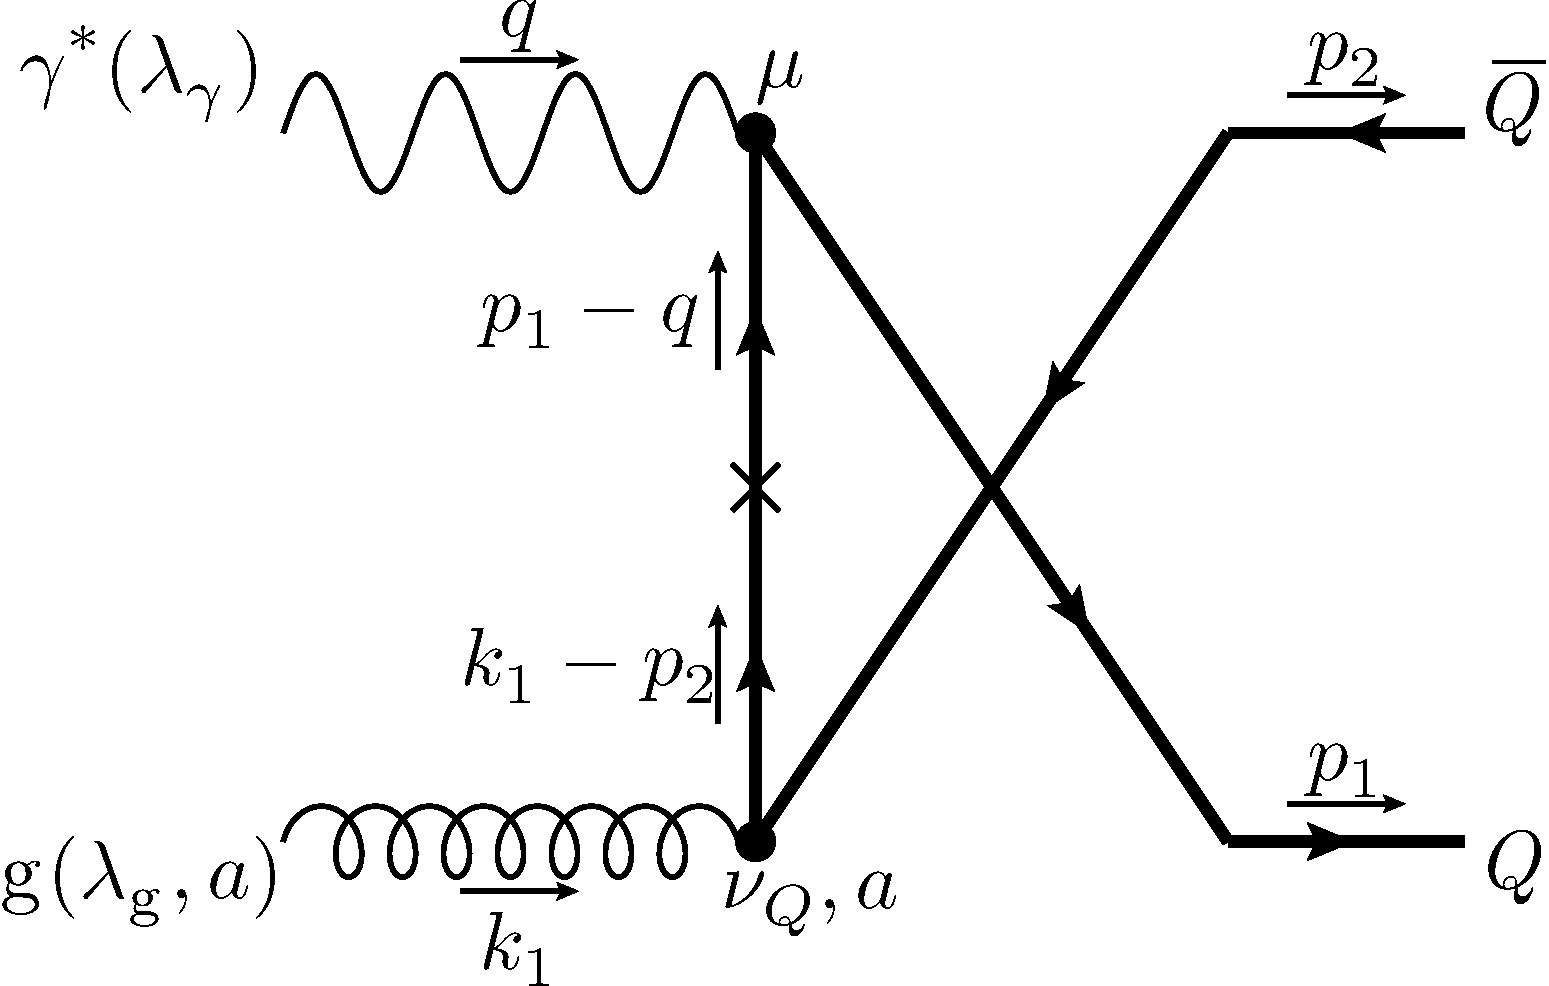
\includegraphics[width=\textwidth]{pyfeyn/nlo-c-mcr}
		\caption{$i\Md^{(NLO,c)}_{2,\mu}$}
	\end{subfigure}\\
	\begin{subfigure}[t]{.4\textwidth}
		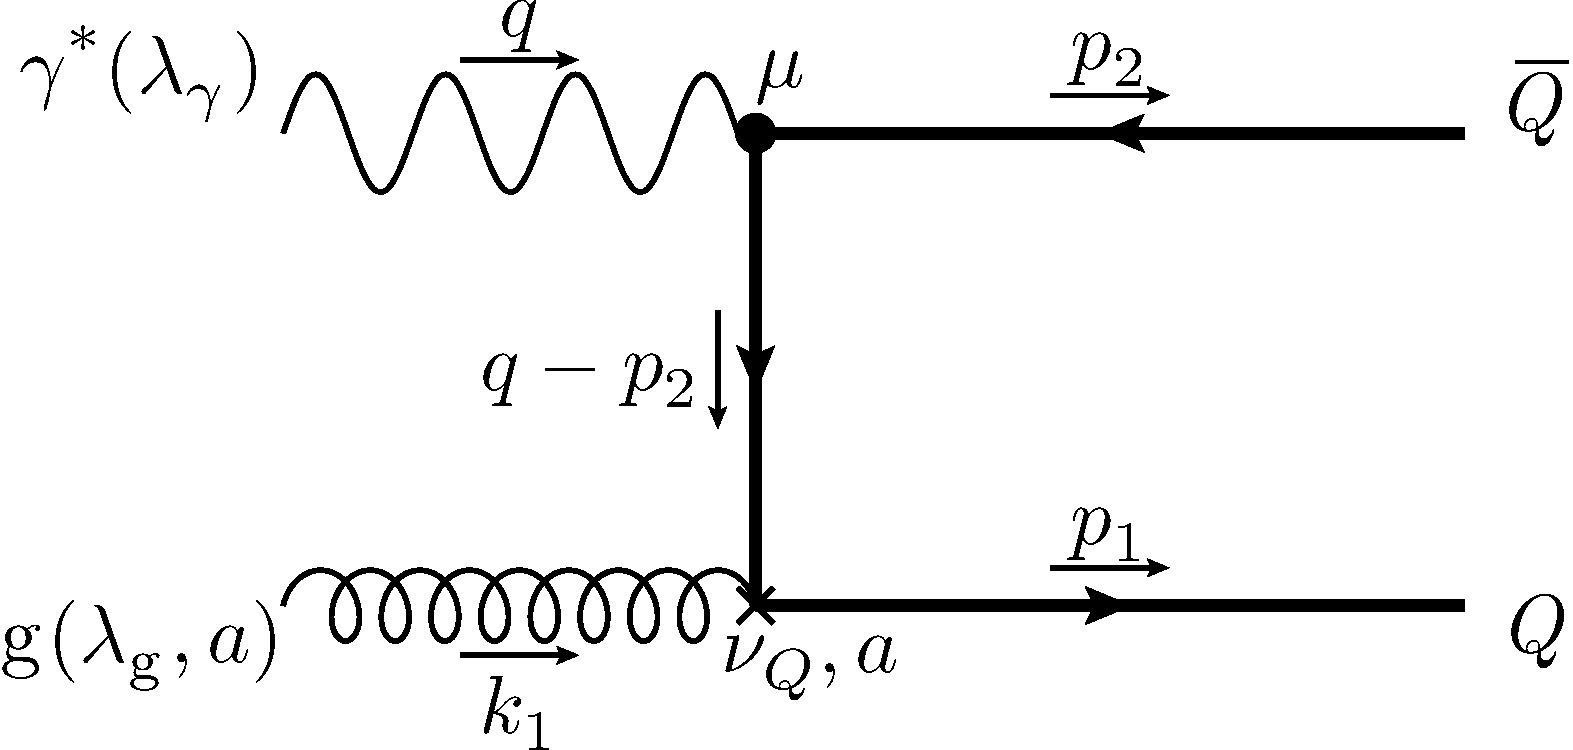
\includegraphics[width=\textwidth]{pyfeyn/nlo-c-nuQ}
		\caption{$i\Md^{(NLO,c)}_{3,\mu}$}
	\end{subfigure}\hspace{.15\textwidth}%
	\begin{subfigure}[t]{.4\textwidth}
		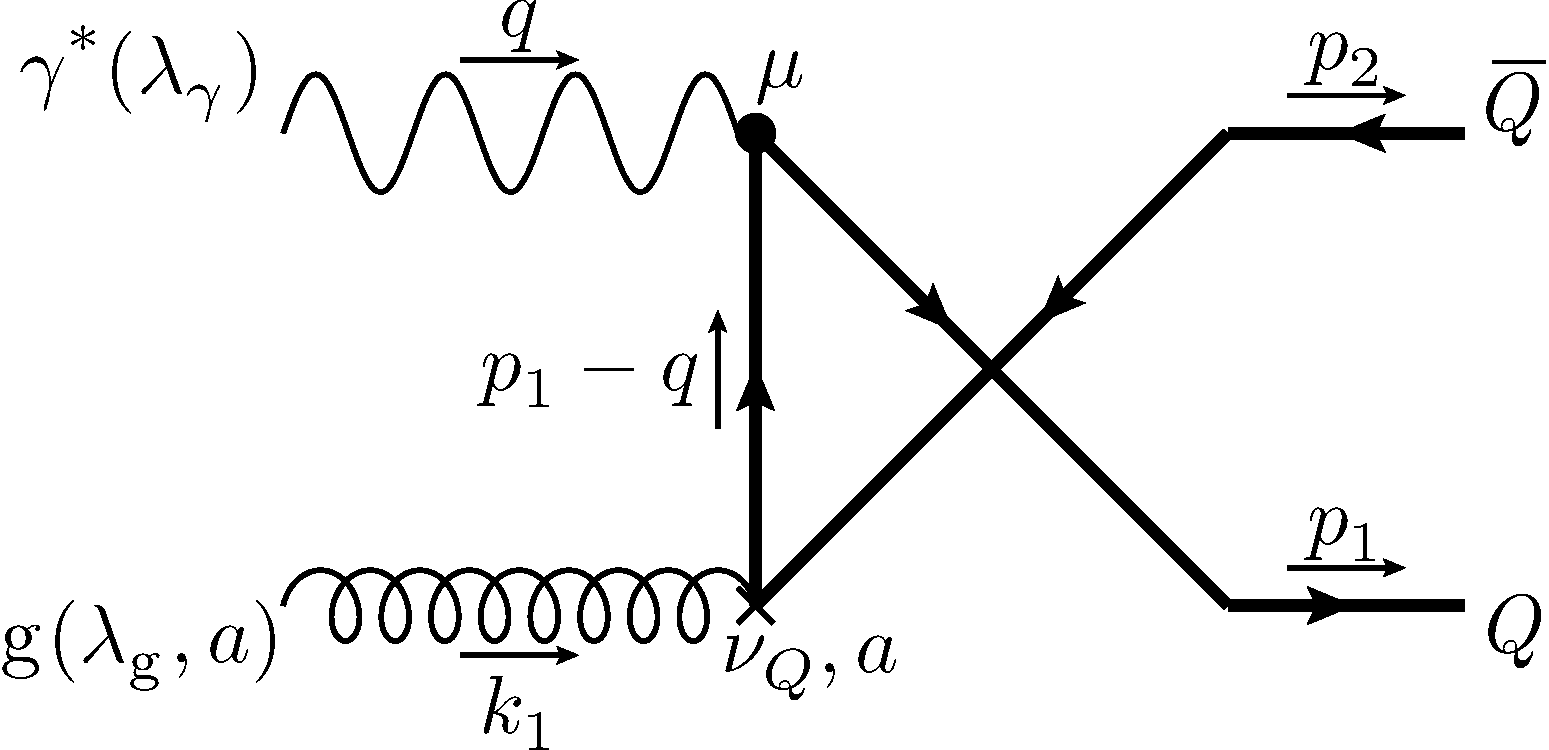
\includegraphics[width=\textwidth]{pyfeyn/nlo-c-nuQcr}
		\caption{$i\Md^{(NLO,c)}_{4,\mu}$}
	\end{subfigure}
	\caption{NLO contributions by counter terms}\label{fig:FeynNLOvf}
\end{figure}

\begin{align}
-i\Md^{(NLO,c)}_{1,\mu} &=\bar u(p_1)(igT_a\gamma^{\nu_Q})\frac{i(\slashed{p}_1-\slashed{k}_1+m)}{t_1}\left(i((Z_2-1)(\slashed{q} - \slashed{p}_2- m) - (Z_m-1)m)\right)\nonumber\\
&\hspace{40pt}\frac{i(\slashed{q}-\slashed{p}_2+m)}{t_1}(-i e e_H \gamma_\mu)v(p_2)\varepsilon^{(\lambda_{\Pg})}_{\nu_Q}(k_1)\\
-i\Md^{(NLO,c)}_{2,\mu} &=\bar u(p_1)(-i e e_H \gamma_\mu)\frac{i(\slashed{p}_1-\slashed{q}+m)}{u_1}\left(i((Z_2-1)(\slashed{p}_1 - \slashed{q}- m) - (Z_m-1)m)\right)\nonumber\\
&\hspace{40pt}\frac{i(\slashed{k}_1-\slashed{p}_2+m)}{u_1}(igT_a\gamma^{\nu_Q})v(p_2)\varepsilon^{(\lambda_{\Pg})}_{\nu_Q}(k_1)\\
-i\Md^{(NLO,c)}_{3,\mu} &=\bar u(p_1)(-i(Z_{1f}-1)gT_a\gamma^{\nu_Q})\frac{i(\slashed{q}-\slashed{p}_2+m)}{u_1}(-i e e_H \gamma_\mu)v(p_2)\varepsilon^{(\lambda_{\Pg})}_{\nu_Q}(k_1)\\
-i\Md^{(NLO,c)}_{4,\mu} &=\bar u(p_1)(-i e e_H \gamma_\mu)\frac{i(\slashed{p}_1-\slashed{q}+m)}{t_1}(-i(Z_{1f}-1)gT_a\gamma^{\nu_Q})v(p_2)\varepsilon^{(\lambda_{\Pg})}_{\nu_Q}(k_1)
\end{align}

Color space:
\begin{align}
\left(\Md^{(NLO,v)}_{1,\mu}+\Md^{(NLO,v)}_{2,\mu}\right)\left(\Md^{(LO)}_{1,\mu'}+\Md^{(LO)}_{2,\mu'}\right)^*&\sim -i\tr(T_aT_bT_aT_b) = -iN_C C_F \left(C_F - \frac{C_A}{2}\right)\\
\left(\Md^{(NLO,v)}_{3,\mu}\right)\left(\Md^{(LO)}_{1,\mu'}+\Md^{(LO)}_{2,\mu'}\right)^*&\sim f_{abc}\tr(T_cT_bT_a) = -\frac i 2 N_C C_F C_A\\
\left(\Md^{(NLO,v)}_{5,\mu}+\Md^{(NLO,v)}_{6,\mu}\right)\left(\Md^{(LO)}_{1,\mu'}+\Md^{(LO)}_{2,\mu'}\right)^*&\sim -i\tr(T_aT_aT_bT_b) = -iN_C C_F^2\\
\end{align}

To compute self energies, we follow \cite{Bojak:2000eu}.
It is
\begin{align}
\{\gamma_\mu,\gamma_\nu\} &= 2g_{\mu\nu}\\
\gamma_\mu\gamma^\mu &= g_\mu^\mu = n \\
\gamma_\mu\gamma_\nu\gamma^\mu &= (2-n)\gamma_\nu
\end{align}
\begin{figure}[ht!]
	\begin{subfigure}[t]{.4\textwidth}
		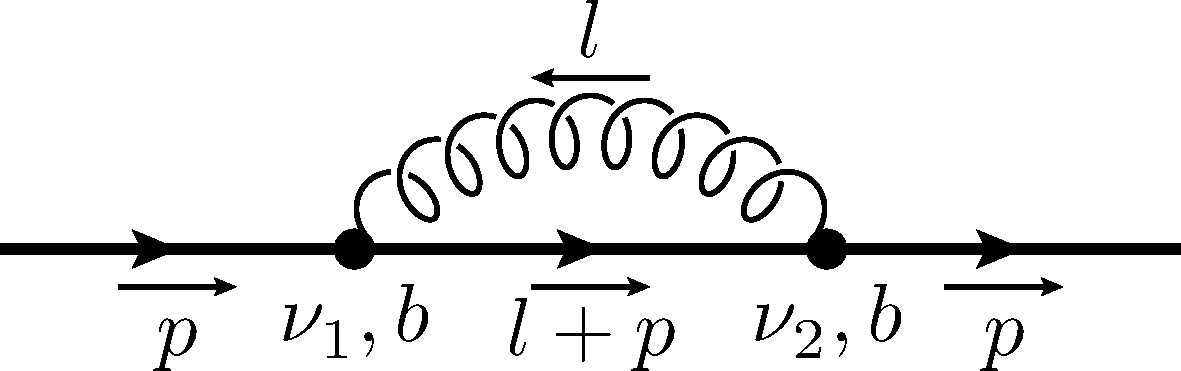
\includegraphics[width=\textwidth]{pyfeyn/nlo-v-seq}
		\caption{$-i\Sigma(p)$}
	\end{subfigure}\hspace{.15\textwidth}%
	\begin{subfigure}[t]{.4\textwidth}
		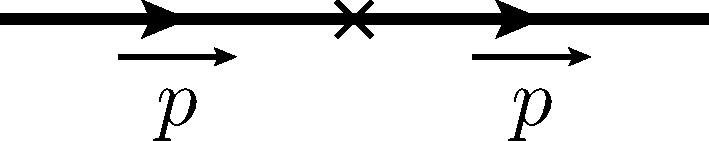
\includegraphics[width=\textwidth]{pyfeyn/nlo-v-seqc}
		\caption{$-i\Sigma_C(p)$}
	\end{subfigure}
	\caption{NLO contributions by quark self energy}\label{fig:FeynNLOvseq}
\end{figure}
\begin{align}
-i\Sigma(p) &= \mu_R^{4-n}\!\!\int\!\!\frac{d^nl}{(2\pi)^n}(igT_b \gamma_{\nu_1})\frac{i(\slashed{l}+\slashed{p}+m)}{(l+p)^2-m^2}(igT_b \gamma_{\nu_2})\frac{-ig^{\nu_1,\nu_2}}{l^2}\\
 &=-\mu_R^{4-n}g^2C_F\!\!\int\!\!\frac{d^nl}{(2\pi)^n}\frac{2m+(2-n)\slashed{p}+(2-n)\slashed{l}}{l^2((l+p)^2-m^2)}\\
 &=-g^2C_F\left(\left(2m+(2-n)\slashed{p}\right)B_0(p^2,0,m^2)+(2-n)B_1(p^2,0,m^2)\right)\\
 &=-g^2C_F\left(B_0(p^2,0,m^2)\left(n\cdot m+(2-n)\slashed{p}\frac{p^2+m^2}{2p^2}\right)-(2-n)\slashed{p}\frac 1{2p^2}A_0(m^2)\right)
\end{align}
Using \cite{Bojak:2000eu} we find
\begin{align}
C_\epsilon &= \frac 1 {16\pi^2}\exp\left(\left(\gamma_E-\log(4\pi)\right)\frac{\epsilon} 2\right)\left(m^2/\mu^2\right)^{\epsilon/2}\\
A_0(m^2) &=iC_\epsilon\left(-\frac 2 {\epsilon}+1\right)\\
B_0(p^2,0,m^2) &=iC_\epsilon\left(-\frac 2{\epsilon}+2+\frac{m^2-p^2}{p^2}\ln\left(\frac{m^2-p^2}{m^2}\right)\right)
\end{align}
\begin{align}
\Rightarrow-i\Sigma(p) &= -ig^2C_FC_\epsilon\left[\frac{2\slashed{p}-8m}{\epsilon}+2m\left(3-2\left(1-\frac{m^2}{p^2}\right)\ln\left(1-\frac{p^2}{m^2}\right)\right)\right.\nonumber\\
 &\hspace{90pt}\left.-\slashed{p}\left(1+\frac{m^2}{p^2}\right)\left(1-\left(1-\frac{m^2}{p^2}\right)\ln\left(1-\frac{p^2}{m^2}\right)\right)\right]\\
 &\EqualClaim -i(A m + B(\slashed p - m))
\end{align}
\begin{align}
\Rightarrow A &= \frac 1 m \left.\Sigma(p)\right|_{\slashed{p}=m} \\
 &= -g^2C_F C_\epsilon\left(\frac 6 \epsilon -5 +\frac{m^2}{p^2}+\left(3-4\frac{m^2}{p^2}+\frac{m^4}{p^4}\right)\ln\left(1-\frac{p^2}{m^2}\right)\right)\\
\Rightarrow B &= \frac 1 m \left.\DeriveF{\slashed{p}}{\Sigma(p)}\right|_{\slashed{p}=m} \\
 &= g^2C_F C_\epsilon\left(\frac 2 \epsilon -1-\frac{m^2}{p^2}+\left(1-\frac{m^4}{p^4}\right)\ln\left(1-\frac{p^2}{m^2}\right)\right)
\end{align}

Counterterm:
\begin{align}
-i\Sigma_C(p) &=i((Z_2-1)\slashed{p}-(Z_2 Z_m -1) m)\\
 &= i((Z_2-1)(\slashed p - m) - (Z_m-1)m) + O(\alpha_S^2)
\end{align}

Use on-shell renormalisation:
\begin{align}
0 &\EqualClaim \left.\left(-i\Sigma(p)-i\Sigma_C(p)\right)\right|_{\slashed{p}=m}\\
 &= i\left.\left(((Z_m-1)+A)m+(B-(Z_2-1))(\slashed p - m)\right)\right|_{\slashed{p}=m} \\
\Rightarrow (Z_m-1) &= \left.-A\right|_{\slashed{p}=m}\\
 &= g^2C_F C_\epsilon\left(\frac 6 \epsilon -4\right)
\end{align}



\newpage
\appendix

\bibliography{ref.bib}
\listoffixmes

\end{document}
